\chapter{Speed Advisory}\label{ch:app}

% \begin{Summary}[Bibliographical Notes]
% This chapter is partially based on the following paper in which the author was the principal investigator:

% \cite{matthes2022selecting} \fullcite{matthes2022selecting}
% \end{Summary}

\section{Introduction}

Diverse solutions have been recently developed to make cycling smarter and increase comfort. One solution explored is warning cyclists of acute dangers along their pathway using crowdsourced data\footnote{Project Rad im Fokus: \url{https://www.synchrone-mobilitaet.de/de/projekte/rad-im-fokus.html}}. Cycling data is also used to determine accident hotspots \cite{von_stulpnagel_crash_2022}, traffic volume \cite{lissner_modeling_2018}, and cycling behavior \cite{lisner_gps-data_2020}, helping transport planners to improve infrastructure where needed. Besides targeted infrastructure enhancement, cooperative cycling and allowing cyclists to form platoons have also been recently explored as a solution to bring cyclists together, focusing on the community aspect of cycling \cite{cespedes_group_2019, meng_connected_2022}.

Given a more individualized perspective, not only bad infrastructure but also stopping at traffic lights is considered a key discomfort factor for cyclists \cite{otto_framework_2023}. Thus, several solutions are currently being tested that aim at reducing stops at intersections. One currently researched option is smartphone applications that act as virtual cyclist detectors for traffic lights, switching green phases as soon as the cyclist arrives at the intersection whenever possible\footnote{Project SiBike (now YuBike): \url{https://www.de.digital/DIGITAL/Redaktion/DE/Smart-City-Navigator/Projekte/sibike-app.html}}. A more passive option is employing static info boards, LED lines, or other visual cues at intersections that help cyclists adjust their speeds \cite{de_angelis_green_2019}. In a recent project, "Leezenflow," researchers were able to achieve a 6.6\% stop reduction at one traffic light in Münster that was equipped with a countdown timer \cite{brand_riding_2024}, leading to a 75.9\% perceived increase in cycling quality. This research is related to studies on green signal countdown devices (GSCDs) installed mainly in the US and China to reduce dilemma zones \cite{lum_before-and-after_2006, huang_evaluating_2014, ni_estimating_2014, chen_exploring_2015, islam_improved_2016}. 

A non-static option is the deployment of a GLOSA application to cyclists. Compared to static info boards, such an application has the potential to be applied to thousands of traffic lights without larger financial expenses, provide a more individual speed advisory, and act as a smart platform for other cycling services. Thus, a mobile application can be seen as advantageous in many ways. The goal of this chapter is to develop such a solution for cyclists, deploy this solution in the large-scale urban environment of Hamburg, and test its impacts. To achieve this solution, we will reuse the developed foundations from \Cref{ch:prediction} (traffic light prediction), \Cref{ch:matching} (traffic light matching), and \Cref{ch:routing} (accurate bike routing).

First, we will study previous GLOSA applications with a focus on developed user interfaces. Among a general study of ways to communicate a speed advisory, we will also discuss previous results regarding usability and cognitive load. Afterward, we will focus on impacts that have been reported in previous works for motorized vehicles and cyclists. Our concept focuses on identifying the best user interface for cyclist speed advisory, and presents auxiliary features that aim at maximizing the app's usability. A final application architecture is presented, highlighting the integration of previously developed services. A usability analysis aims to identify the perceived benefits and drawbacks of our developed mobile application during extensive long-term field tests. This qualitative study is supplemented with a thorough analysis of user trajectories, including an evaluation of stop reduction and estimated energy savings. With our results from the qualitative and quantitative study, we conclude the impacts of our developed speed advisory on cyclists. 

\section{Related Work}\label{sec:rw-uis}

Studies on the effect of a traffic light speed advisory have been conducted in various different experimental contexts. As a result, diverse user interfaces and measurements of the speed advisory's impact have been contributed over time. 

While traffic-light-predictive cruise control systems have been demonstrated which directly influence a vehicle's powertrain \cite{raubitschek_predictive_2011}, the user interface can be seen as an integral part of GLOSA systems. However, the relation between a user interface and reaction to a speed advisory has not always been tested in correspondence, meaning that many studies have been conducted without a human in the loop. To emulate a reaction to the speed advisory, simulation studies typically utilize a driver model \cite{hu_lane-level_2023}, including the vehicle's acceleration behavior and, occasionally, additional factors such as human interaction delay \cite{schlamp_2023_glosa}. Another dimension is introduced by studies that investigate the impact of a speed-advised lead vehicle onto subsequent vehicles \cite{preuk_does_2016, preuk_should_2018}. In many of these studies, constant user obedience and a usable speed advisory are assumed.

However, there has also been recent criticism about the realism of many of the conducted simulation studies. Klöppel et al. (2019) \cite{kloeppel_performance_2019} conclude that individual aspects required for a realistic impact simulation are often neglected. Many studies that have painted an optimistic picture of potential effects fall short of depicting a realistic response to the speed advisory, according to the authors. Due to these limitations, the demand for holistic, real-world studies has increased \cite{stahlmann_exploring_2018}. Such a holistic study must also consider the user interface and its guidance efficacy. 

The following sections will explore the research on speed advisory from different perspectives. First, we will look at the diverse landscape of possible user interfaces, identifying the drawbacks and advantages for cyclist applications. Broadening the view towards non-visual interfaces allows us to identify new ideas to convey a speed advisory. Previous experiments with speed advisory on cyclists and usability studies are discussed, inferring current challenges and knowledge gaps that could be addressed with a novel design. Finally, we summarize the reported effects of the speed advisory on traffic participants in relation to experimental circumstances. The reported energy savings and stop reductions will serve as a baseline at the end of this chapter.

\subsection{User Interfaces}

Diverse user interfaces have been proposed over time to present a traffic light speed advisory. Often, multiple interfaces are tested in conjunction.

In various studies, a target speed is directly recommended. Otto et al. (2010) \cite{otto_operating_2010} employ speed signs, similar to those found on the roadside, to encourage users to slow down when approaching a red traffic light at normal driving speed. Koukoumidis et al. (2011) \cite{koukoumidis_signalguru_2011, koukoumidis_leveraging_2012} recommend a specific speed, presenting the recommendation not only as a speed limit but also as an acceleration suggestion. Mahler et al. (2012) \cite{mahler_reducing_2012} adopt a similar approach. Zweck et al. (2013) \cite{zweck_traffic_2013} demonstrate the implementation of target speed recommendation in an Audi's onboard computer. Olaverri-Monreal et al. (2018) \cite{olaverri-monreal_implementation_2018} show a similar integrated visualization in the onboard computer of a simulated vehicle. BMW's EnLighten System also utilizes an infotainment display, as indicated by Sokolov et al. (2018) \cite{sokolov_effects_2018}. Except for integration methods, these approaches share similar design principles. In the background, a model determines the best achievable green phase and calculates the required target speed, which is then presented more or less directly in textual form.

Some works apply a slight variation to the target speed advisory user interface, such as in a work by Parella (2019) \cite{marias_parella_design_2019}, where the target speed is marked on the speedometer instead of being displayed as text. Xu et al. (2015) \cite{xu_bb_2015} demonstrate a hybrid approach based on a target speed advisory using auditory prompts. Vibration-based inputs for speed recommendations are also discussed, particularly in cycling contexts \cite{cespedes_group_2019}, though not extensively explored in the context of GLOSA. The Signal2X App by Yunex \cite{yunex_traffic_v2x-kommunikation_2023} and Bhattacharyya et al. (2022) \cite{bhattacharyya_assessing_2022} not only display target speed for a single but also for multiple parallel traffic lights. Another variation in target speed advisory is found in the cycling study by Fickas et al. (2019) \cite{fickas_fast_2019}. Instead of displaying the target speed, arrows indicate weak or strong acceleration or braking recommendations to achieve the target speed. However, the situational awareness of this approach was found to be an issue, especially in hilly terrain or other challenging situations.

The second most common visualization is the countdown to the next traffic light change (Time-to-Green or Time-to-Red). This method is simpler, requiring no model for green phase selection or precise distance estimation to the traffic light. Usually, a countdown is presented alongside the target speed \cite{koukoumidis_signalguru_2011, koukoumidis_leveraging_2012}. Audi's GLOSA system, for example, switches from displaying the target speed to the countdown when the vehicle is stationary at a traffic light \cite{zweck_traffic_2013}. BMW's EnLighten System also features both target speed and countdown displays \cite{sokolov_effects_2018}. When standing at the red light, the countdown is typically hidden five seconds before the traffic light switches to avoid premature acceleration \cite{stahlmann_exploring_2018, sokolov_effects_2018}. Otto et al. (2010) \cite{otto_operating_2010} demonstrate the feasibility of visualizing information for multiple parallel lanes, a concept also implemented by Jacob et al. (2020) \cite{jacob_ivs-kom_2020}, Khan et al. (2021) \cite{khan_eco-drive_2021}, and the Yunex Signal2X App \cite{yunex_traffic_v2x-kommunikation_2023}. Some studies accompany the countdown with auditory signals. Chen et al. (2022) \cite{chen_developing_2022} audibly convey the countdown every 2 seconds to the user. Wilson et al. (2017) \cite{wilson_driver_2017} tested an auditory warning and a "Prepare to Go" signal, indicating an imminent traffic light change.

The third most popular visual representation of speed recommendation involves projective methods, where the traffic light prediction is projected onto the road (Lane Projection, Carpet) or onto a speedometer. While a specific speed is not selected, an accurate distance estimate and prediction of multiple phases are required. The Carpet visualization, initially proposed by Otto et al. (2010) \cite{otto_operating_2010}, involves shifting a prediction carpet through acceleration or deceleration to stay within the green phase, resembling a green wave on which users can "jump on." This method allows for visualizing uncertainties in the prediction by blurring the phase areas, a large advantage over countdowns or target speed displays. Bernais et al. (2016) \cite{bernais_design_2016} also utilize this visualization, modifying it to display multiple lane carpets side by side. Suzuki et al. (2018 -- 2020) \cite{suzuki_new_2018, suzuki_safety_2020} demonstrate that this visualization method can also be implemented in a car's heads-up display by projecting the carpet's colors into the driver's field of view. Besides the carpet visualization, the speedometer visualization operates quite similarly, projecting the prediction along speeds on the speedometer's speed arc. This method was first tested in the field by Xia et al. (2012) \cite{xia_field_2012} and later reused by Hao et al. (2019) \cite{hao_eco-approach_2019}. Parella (2019) \cite{marias_parella_design_2019} shows a combination of target speed and speedometer.

Except for countdown visualization, Krause et al. (2012) \cite{krause_traffic_2012} investigated the usability and distraction of these visualizations. Two additional visualization types, "Fisheye" and "Roll," were introduced, similar to the evaluated Carpet projection but with a colored number band instead of a colored surface area. Usability was evaluated using the System Usability Scale (SUS) and the AttrakDiff Score. The speedometer projection scored the highest with a SUS of 80.4, followed by the Carpet visualization (75.3), Roll (73.9), Fisheye (58.8), and target speed recommendation (56.5). The AttrakDiff Score mirrored these results. While target speed recommendation, the most frequently used visualization, performed poorly in terms of usability, the Speedometer method emerged as the most promising in the simulator experiment. Krause et al. (2012) \cite{krause_traffic_2012} also examined the impact of visualization on distraction. Users spent the least time looking at the poorly rated target speed recommendation, although the off-road glance duration was, in part, longer, potentially due to shifting focus between the recommended speed and the vehicle speedometer. Minimal differences were observed between the other visualizations, indicating no clear winner.

The studies by Krause et al. (2012) \cite{krause_traffic_2012} and findings by Fickas et al. (2019) \cite{fickas_fast_2019} suggest that target speed recommendation is likely not a good option, while the less explored speedometer visualization appears most promising in terms of usability. Few studies, apart from Wilson et al. (2017) \cite{wilson_driver_2017}, have investigated usability, with the SUS score testing BMW's EnLighten System at an average of 71.4 (SD = 12.6). However, this study identified various factors negatively affecting usability, notably the loss of GNSS connectivity during driving. Thus, user acceptance of a speed recommendation app depends not only on the visualization method but also on the overall functionality of the app.

Different approaches have been explored for integrating speed recommendations into overall systems. In works by Xia et al. (2012) \cite{xia_field_2012}, Zweck et al. (2013) \cite{zweck_traffic_2013}, and later by Stahlmann et al. (2018) \cite{stahlmann_exploring_2018}, the focus is on the overall vehicle system. The speed recommendation is linked with other infotainment components and receives crucial additional information, such as turn signal status, from the vehicle information system, as seen in Audi's system. BMW's EnLighten System was tested in two forms: as an integrated system in the vehicle \cite{sokolov_effects_2018} and previously as a mobile app \cite{wilson_driver_2017}, presumably using the smartphone as a prototyping environment. Smartphone app development has often followed a "ride as you go" approach \cite{otto_operating_2010, koukoumidis_signalguru_2011, koukoumidis_leveraging_2012, bernais_design_2016, wilson_driver_2017, zhang_green_2020, khan_eco-drive_2021, yunex_traffic_v2x-kommunikation_2023}. This approach allows users to start driving without choosing a route beforehand. However, several works reported issues with GNSS accuracy, especially in traffic light selection \cite{wilson_driver_2017, stahlmann_exploring_2018, bhattacharyya_assessing_2022}.

Mahler et al. (2012) \cite{mahler_reducing_2012} proposed an alternative approach: instead of starting immediately, users should specify a route before driving. This allows the app to preselect traffic lights along the route. The advantages of such an approach were discussed in \Cref{ch:matching} and \Cref{ch:routing}. Another indication of the potential suboptimality of the Ride-as-you-go approach comes from user reviews of the TrafficPilot App, where the ability to calculate routes is frequently perceived as a missing feature.

Two recent works demonstrate how such integration could look. Bhattacharyya et al. (2022) \cite{bhattacharyya_assessing_2022}, associated with the CTD App, presents GLOSA as a component of a connected navigation app. The app switches between different functional views in various situations, displaying recommended speeds on parallel lanes as the vehicle approaches an intersection. In a recent study by Ding et al. (2023) \cite{ding_speedadv_2023}, the presentation is integrated as an additional element in a navigation app, showing a small circle with the target speed. The relevant traffic light for turning is also selected.

Thus, a combination of GLOSA and a navigation app seems to be a promising current approach, although few insights are available on how well existing GLOSA systems are received by users.

\subsection{Impacts}

\begin{figure}
\centering
\resizebox{\linewidth}{!}{%
%% Creator: Matplotlib, PGF backend
%%
%% To include the figure in your LaTeX document, write
%%   \input{<filename>.pgf}
%%
%% Make sure the required packages are loaded in your preamble
%%   \usepackage{pgf}
%%
%% Also ensure that all the required font packages are loaded; for instance,
%% the lmodern package is sometimes necessary when using math font.
%%   \usepackage{lmodern}
%%
%% Figures using additional raster images can only be included by \input if
%% they are in the same directory as the main LaTeX file. For loading figures
%% from other directories you can use the `import` package
%%   \usepackage{import}
%%
%% and then include the figures with
%%   \import{<path to file>}{<filename>.pgf}
%%
%% Matplotlib used the following preamble
%%   \def\mathdefault#1{#1}
%%   \everymath=\expandafter{\the\everymath\displaystyle}
%%   
%%   \makeatletter\@ifpackageloaded{underscore}{}{\usepackage[strings]{underscore}}\makeatother
%%
\begingroup%
\makeatletter%
\begin{pgfpicture}%
\pgfpathrectangle{\pgfpointorigin}{\pgfqpoint{6.900001in}{3.152360in}}%
\pgfusepath{use as bounding box, clip}%
\begin{pgfscope}%
\pgfsetbuttcap%
\pgfsetmiterjoin%
\definecolor{currentfill}{rgb}{1.000000,1.000000,1.000000}%
\pgfsetfillcolor{currentfill}%
\pgfsetlinewidth{0.000000pt}%
\definecolor{currentstroke}{rgb}{1.000000,1.000000,1.000000}%
\pgfsetstrokecolor{currentstroke}%
\pgfsetdash{}{0pt}%
\pgfpathmoveto{\pgfqpoint{0.000000in}{0.000000in}}%
\pgfpathlineto{\pgfqpoint{6.900001in}{0.000000in}}%
\pgfpathlineto{\pgfqpoint{6.900001in}{3.152360in}}%
\pgfpathlineto{\pgfqpoint{0.000000in}{3.152360in}}%
\pgfpathlineto{\pgfqpoint{0.000000in}{0.000000in}}%
\pgfpathclose%
\pgfusepath{fill}%
\end{pgfscope}%
\begin{pgfscope}%
\pgfsetbuttcap%
\pgfsetmiterjoin%
\definecolor{currentfill}{rgb}{1.000000,1.000000,1.000000}%
\pgfsetfillcolor{currentfill}%
\pgfsetlinewidth{0.000000pt}%
\definecolor{currentstroke}{rgb}{0.000000,0.000000,0.000000}%
\pgfsetstrokecolor{currentstroke}%
\pgfsetstrokeopacity{0.000000}%
\pgfsetdash{}{0pt}%
\pgfpathmoveto{\pgfqpoint{0.600001in}{0.742360in}}%
\pgfpathlineto{\pgfqpoint{6.800001in}{0.742360in}}%
\pgfpathlineto{\pgfqpoint{6.800001in}{3.052360in}}%
\pgfpathlineto{\pgfqpoint{0.600001in}{3.052360in}}%
\pgfpathlineto{\pgfqpoint{0.600001in}{0.742360in}}%
\pgfpathclose%
\pgfusepath{fill}%
\end{pgfscope}%
\begin{pgfscope}%
\pgfpathrectangle{\pgfqpoint{0.600001in}{0.742360in}}{\pgfqpoint{6.200000in}{2.310000in}}%
\pgfusepath{clip}%
\pgfsetbuttcap%
\pgfsetroundjoin%
\definecolor{currentfill}{rgb}{0.000000,0.450980,1.000000}%
\pgfsetfillcolor{currentfill}%
\pgfsetlinewidth{1.505625pt}%
\definecolor{currentstroke}{rgb}{0.000000,0.450980,1.000000}%
\pgfsetstrokecolor{currentstroke}%
\pgfsetdash{}{0pt}%
\pgfsys@defobject{currentmarker}{\pgfqpoint{-0.049105in}{-0.049105in}}{\pgfqpoint{0.049105in}{0.049105in}}{%
\pgfpathmoveto{\pgfqpoint{-0.049105in}{0.000000in}}%
\pgfpathlineto{\pgfqpoint{0.049105in}{0.000000in}}%
\pgfpathmoveto{\pgfqpoint{0.000000in}{-0.049105in}}%
\pgfpathlineto{\pgfqpoint{0.000000in}{0.049105in}}%
\pgfusepath{stroke,fill}%
}%
\begin{pgfscope}%
\pgfsys@transformshift{0.881819in}{2.268885in}%
\pgfsys@useobject{currentmarker}{}%
\end{pgfscope}%
\begin{pgfscope}%
\pgfsys@transformshift{1.063637in}{2.089860in}%
\pgfsys@useobject{currentmarker}{}%
\end{pgfscope}%
\begin{pgfscope}%
\pgfsys@transformshift{1.063637in}{2.205360in}%
\pgfsys@useobject{currentmarker}{}%
\end{pgfscope}%
\begin{pgfscope}%
\pgfsys@transformshift{1.245455in}{1.839610in}%
\pgfsys@useobject{currentmarker}{}%
\end{pgfscope}%
\begin{pgfscope}%
\pgfsys@transformshift{1.245455in}{2.012860in}%
\pgfsys@useobject{currentmarker}{}%
\end{pgfscope}%
\begin{pgfscope}%
\pgfsys@transformshift{1.427273in}{1.550860in}%
\pgfsys@useobject{currentmarker}{}%
\end{pgfscope}%
\begin{pgfscope}%
\pgfsys@transformshift{1.427273in}{1.820360in}%
\pgfsys@useobject{currentmarker}{}%
\end{pgfscope}%
\begin{pgfscope}%
\pgfsys@transformshift{1.609092in}{1.668285in}%
\pgfsys@useobject{currentmarker}{}%
\end{pgfscope}%
\begin{pgfscope}%
\pgfsys@transformshift{1.790910in}{1.604760in}%
\pgfsys@useobject{currentmarker}{}%
\end{pgfscope}%
\begin{pgfscope}%
\pgfsys@transformshift{1.972728in}{1.512360in}%
\pgfsys@useobject{currentmarker}{}%
\end{pgfscope}%
\begin{pgfscope}%
\pgfsys@transformshift{2.154546in}{1.377610in}%
\pgfsys@useobject{currentmarker}{}%
\end{pgfscope}%
\begin{pgfscope}%
\pgfsys@transformshift{2.154546in}{1.535460in}%
\pgfsys@useobject{currentmarker}{}%
\end{pgfscope}%
\begin{pgfscope}%
\pgfsys@transformshift{2.336364in}{1.416110in}%
\pgfsys@useobject{currentmarker}{}%
\end{pgfscope}%
\begin{pgfscope}%
\pgfsys@transformshift{2.518183in}{1.752985in}%
\pgfsys@useobject{currentmarker}{}%
\end{pgfscope}%
\begin{pgfscope}%
\pgfsys@transformshift{2.518183in}{0.992610in}%
\pgfsys@useobject{currentmarker}{}%
\end{pgfscope}%
\begin{pgfscope}%
\pgfsys@transformshift{2.700001in}{1.360285in}%
\pgfsys@useobject{currentmarker}{}%
\end{pgfscope}%
\begin{pgfscope}%
\pgfsys@transformshift{2.881819in}{1.339110in}%
\pgfsys@useobject{currentmarker}{}%
\end{pgfscope}%
\begin{pgfscope}%
\pgfsys@transformshift{3.063637in}{1.325635in}%
\pgfsys@useobject{currentmarker}{}%
\end{pgfscope}%
\begin{pgfscope}%
\pgfsys@transformshift{3.245455in}{1.262110in}%
\pgfsys@useobject{currentmarker}{}%
\end{pgfscope}%
\begin{pgfscope}%
\pgfsys@transformshift{3.427273in}{1.225535in}%
\pgfsys@useobject{currentmarker}{}%
\end{pgfscope}%
\begin{pgfscope}%
\pgfsys@transformshift{3.609092in}{1.088860in}%
\pgfsys@useobject{currentmarker}{}%
\end{pgfscope}%
\begin{pgfscope}%
\pgfsys@transformshift{3.609092in}{1.358360in}%
\pgfsys@useobject{currentmarker}{}%
\end{pgfscope}%
\begin{pgfscope}%
\pgfsys@transformshift{3.790910in}{1.196468in}%
\pgfsys@useobject{currentmarker}{}%
\end{pgfscope}%
\begin{pgfscope}%
\pgfsys@transformshift{3.972728in}{1.156235in}%
\pgfsys@useobject{currentmarker}{}%
\end{pgfscope}%
\begin{pgfscope}%
\pgfsys@transformshift{4.154546in}{1.146610in}%
\pgfsys@useobject{currentmarker}{}%
\end{pgfscope}%
\begin{pgfscope}%
\pgfsys@transformshift{4.336364in}{1.129285in}%
\pgfsys@useobject{currentmarker}{}%
\end{pgfscope}%
\begin{pgfscope}%
\pgfsys@transformshift{4.518183in}{1.127360in}%
\pgfsys@useobject{currentmarker}{}%
\end{pgfscope}%
\begin{pgfscope}%
\pgfsys@transformshift{4.700001in}{1.113308in}%
\pgfsys@useobject{currentmarker}{}%
\end{pgfscope}%
\begin{pgfscope}%
\pgfsys@transformshift{4.881819in}{0.992610in}%
\pgfsys@useobject{currentmarker}{}%
\end{pgfscope}%
\begin{pgfscope}%
\pgfsys@transformshift{4.881819in}{1.223610in}%
\pgfsys@useobject{currentmarker}{}%
\end{pgfscope}%
\begin{pgfscope}%
\pgfsys@transformshift{5.063637in}{1.029185in}%
\pgfsys@useobject{currentmarker}{}%
\end{pgfscope}%
\begin{pgfscope}%
\pgfsys@transformshift{5.063637in}{1.162010in}%
\pgfsys@useobject{currentmarker}{}%
\end{pgfscope}%
\begin{pgfscope}%
\pgfsys@transformshift{5.245455in}{1.077310in}%
\pgfsys@useobject{currentmarker}{}%
\end{pgfscope}%
\begin{pgfscope}%
\pgfsys@transformshift{5.427273in}{1.069610in}%
\pgfsys@useobject{currentmarker}{}%
\end{pgfscope}%
\begin{pgfscope}%
\pgfsys@transformshift{5.609092in}{1.050360in}%
\pgfsys@useobject{currentmarker}{}%
\end{pgfscope}%
\begin{pgfscope}%
\pgfsys@transformshift{5.790910in}{1.031110in}%
\pgfsys@useobject{currentmarker}{}%
\end{pgfscope}%
\begin{pgfscope}%
\pgfsys@transformshift{5.972728in}{1.021485in}%
\pgfsys@useobject{currentmarker}{}%
\end{pgfscope}%
\begin{pgfscope}%
\pgfsys@transformshift{6.154546in}{0.992610in}%
\pgfsys@useobject{currentmarker}{}%
\end{pgfscope}%
\begin{pgfscope}%
\pgfsys@transformshift{6.336364in}{0.959885in}%
\pgfsys@useobject{currentmarker}{}%
\end{pgfscope}%
\begin{pgfscope}%
\pgfsys@transformshift{6.336364in}{1.011860in}%
\pgfsys@useobject{currentmarker}{}%
\end{pgfscope}%
\begin{pgfscope}%
\pgfsys@transformshift{6.518183in}{0.944485in}%
\pgfsys@useobject{currentmarker}{}%
\end{pgfscope}%
\end{pgfscope}%
\begin{pgfscope}%
\pgfsetbuttcap%
\pgfsetroundjoin%
\definecolor{currentfill}{rgb}{0.000000,0.000000,0.000000}%
\pgfsetfillcolor{currentfill}%
\pgfsetlinewidth{0.803000pt}%
\definecolor{currentstroke}{rgb}{0.000000,0.000000,0.000000}%
\pgfsetstrokecolor{currentstroke}%
\pgfsetdash{}{0pt}%
\pgfsys@defobject{currentmarker}{\pgfqpoint{0.000000in}{-0.048611in}}{\pgfqpoint{0.000000in}{0.000000in}}{%
\pgfpathmoveto{\pgfqpoint{0.000000in}{0.000000in}}%
\pgfpathlineto{\pgfqpoint{0.000000in}{-0.048611in}}%
\pgfusepath{stroke,fill}%
}%
\begin{pgfscope}%
\pgfsys@transformshift{0.881819in}{0.742360in}%
\pgfsys@useobject{currentmarker}{}%
\end{pgfscope}%
\end{pgfscope}%
\begin{pgfscope}%
\definecolor{textcolor}{rgb}{0.000000,0.000000,0.000000}%
\pgfsetstrokecolor{textcolor}%
\pgfsetfillcolor{textcolor}%
\pgftext[x=0.916541in, y=0.260301in, left, base,rotate=90.000000]{\color{textcolor}{\sffamily\fontsize{10.000000}{12.000000}\selectfont\catcode`\^=\active\def^{\ifmmode\sp\else\^{}\fi}\catcode`\%=\active\def%{\%}\cite{li_multi-vehicles_2014}}}%
\end{pgfscope}%
\begin{pgfscope}%
\pgfsetbuttcap%
\pgfsetroundjoin%
\definecolor{currentfill}{rgb}{0.000000,0.000000,0.000000}%
\pgfsetfillcolor{currentfill}%
\pgfsetlinewidth{0.803000pt}%
\definecolor{currentstroke}{rgb}{0.000000,0.000000,0.000000}%
\pgfsetstrokecolor{currentstroke}%
\pgfsetdash{}{0pt}%
\pgfsys@defobject{currentmarker}{\pgfqpoint{0.000000in}{-0.048611in}}{\pgfqpoint{0.000000in}{0.000000in}}{%
\pgfpathmoveto{\pgfqpoint{0.000000in}{0.000000in}}%
\pgfpathlineto{\pgfqpoint{0.000000in}{-0.048611in}}%
\pgfusepath{stroke,fill}%
}%
\begin{pgfscope}%
\pgfsys@transformshift{1.063637in}{0.742360in}%
\pgfsys@useobject{currentmarker}{}%
\end{pgfscope}%
\end{pgfscope}%
\begin{pgfscope}%
\definecolor{textcolor}{rgb}{0.000000,0.000000,0.000000}%
\pgfsetstrokecolor{textcolor}%
\pgfsetfillcolor{textcolor}%
\pgftext[x=1.098359in, y=0.260301in, left, base,rotate=90.000000]{\color{textcolor}{\sffamily\fontsize{10.000000}{12.000000}\selectfont\catcode`\^=\active\def^{\ifmmode\sp\else\^{}\fi}\catcode`\%=\active\def%{\%}\cite{mahler_reducing_2012}}}%
\end{pgfscope}%
\begin{pgfscope}%
\pgfsetbuttcap%
\pgfsetroundjoin%
\definecolor{currentfill}{rgb}{0.000000,0.000000,0.000000}%
\pgfsetfillcolor{currentfill}%
\pgfsetlinewidth{0.803000pt}%
\definecolor{currentstroke}{rgb}{0.000000,0.000000,0.000000}%
\pgfsetstrokecolor{currentstroke}%
\pgfsetdash{}{0pt}%
\pgfsys@defobject{currentmarker}{\pgfqpoint{0.000000in}{-0.048611in}}{\pgfqpoint{0.000000in}{0.000000in}}{%
\pgfpathmoveto{\pgfqpoint{0.000000in}{0.000000in}}%
\pgfpathlineto{\pgfqpoint{0.000000in}{-0.048611in}}%
\pgfusepath{stroke,fill}%
}%
\begin{pgfscope}%
\pgfsys@transformshift{1.245455in}{0.742360in}%
\pgfsys@useobject{currentmarker}{}%
\end{pgfscope}%
\end{pgfscope}%
\begin{pgfscope}%
\definecolor{textcolor}{rgb}{0.000000,0.000000,0.000000}%
\pgfsetstrokecolor{textcolor}%
\pgfsetfillcolor{textcolor}%
\pgftext[x=1.280177in, y=0.260301in, left, base,rotate=90.000000]{\color{textcolor}{\sffamily\fontsize{10.000000}{12.000000}\selectfont\catcode`\^=\active\def^{\ifmmode\sp\else\^{}\fi}\catcode`\%=\active\def%{\%}\cite{asadi_predictive_2011}}}%
\end{pgfscope}%
\begin{pgfscope}%
\pgfsetbuttcap%
\pgfsetroundjoin%
\definecolor{currentfill}{rgb}{0.000000,0.000000,0.000000}%
\pgfsetfillcolor{currentfill}%
\pgfsetlinewidth{0.803000pt}%
\definecolor{currentstroke}{rgb}{0.000000,0.000000,0.000000}%
\pgfsetstrokecolor{currentstroke}%
\pgfsetdash{}{0pt}%
\pgfsys@defobject{currentmarker}{\pgfqpoint{0.000000in}{-0.048611in}}{\pgfqpoint{0.000000in}{0.000000in}}{%
\pgfpathmoveto{\pgfqpoint{0.000000in}{0.000000in}}%
\pgfpathlineto{\pgfqpoint{0.000000in}{-0.048611in}}%
\pgfusepath{stroke,fill}%
}%
\begin{pgfscope}%
\pgfsys@transformshift{1.427273in}{0.742360in}%
\pgfsys@useobject{currentmarker}{}%
\end{pgfscope}%
\end{pgfscope}%
\begin{pgfscope}%
\definecolor{textcolor}{rgb}{0.000000,0.000000,0.000000}%
\pgfsetstrokecolor{textcolor}%
\pgfsetfillcolor{textcolor}%
\pgftext[x=1.461996in, y=0.260301in, left, base,rotate=90.000000]{\color{textcolor}{\sffamily\fontsize{10.000000}{12.000000}\selectfont\catcode`\^=\active\def^{\ifmmode\sp\else\^{}\fi}\catcode`\%=\active\def%{\%}\cite{tal_vehicular-communications-based_2016}}}%
\end{pgfscope}%
\begin{pgfscope}%
\pgfsetbuttcap%
\pgfsetroundjoin%
\definecolor{currentfill}{rgb}{0.000000,0.000000,0.000000}%
\pgfsetfillcolor{currentfill}%
\pgfsetlinewidth{0.803000pt}%
\definecolor{currentstroke}{rgb}{0.000000,0.000000,0.000000}%
\pgfsetstrokecolor{currentstroke}%
\pgfsetdash{}{0pt}%
\pgfsys@defobject{currentmarker}{\pgfqpoint{0.000000in}{-0.048611in}}{\pgfqpoint{0.000000in}{0.000000in}}{%
\pgfpathmoveto{\pgfqpoint{0.000000in}{0.000000in}}%
\pgfpathlineto{\pgfqpoint{0.000000in}{-0.048611in}}%
\pgfusepath{stroke,fill}%
}%
\begin{pgfscope}%
\pgfsys@transformshift{1.609092in}{0.742360in}%
\pgfsys@useobject{currentmarker}{}%
\end{pgfscope}%
\end{pgfscope}%
\begin{pgfscope}%
\definecolor{textcolor}{rgb}{0.000000,0.000000,0.000000}%
\pgfsetstrokecolor{textcolor}%
\pgfsetfillcolor{textcolor}%
\pgftext[x=1.643814in, y=0.260301in, left, base,rotate=90.000000]{\color{textcolor}{\sffamily\fontsize{10.000000}{12.000000}\selectfont\catcode`\^=\active\def^{\ifmmode\sp\else\^{}\fi}\catcode`\%=\active\def%{\%}\cite{simchon_real-time_2020}}}%
\end{pgfscope}%
\begin{pgfscope}%
\pgfsetbuttcap%
\pgfsetroundjoin%
\definecolor{currentfill}{rgb}{0.000000,0.000000,0.000000}%
\pgfsetfillcolor{currentfill}%
\pgfsetlinewidth{0.803000pt}%
\definecolor{currentstroke}{rgb}{0.000000,0.000000,0.000000}%
\pgfsetstrokecolor{currentstroke}%
\pgfsetdash{}{0pt}%
\pgfsys@defobject{currentmarker}{\pgfqpoint{0.000000in}{-0.048611in}}{\pgfqpoint{0.000000in}{0.000000in}}{%
\pgfpathmoveto{\pgfqpoint{0.000000in}{0.000000in}}%
\pgfpathlineto{\pgfqpoint{0.000000in}{-0.048611in}}%
\pgfusepath{stroke,fill}%
}%
\begin{pgfscope}%
\pgfsys@transformshift{1.790910in}{0.742360in}%
\pgfsys@useobject{currentmarker}{}%
\end{pgfscope}%
\end{pgfscope}%
\begin{pgfscope}%
\definecolor{textcolor}{rgb}{0.000000,0.000000,0.000000}%
\pgfsetstrokecolor{textcolor}%
\pgfsetfillcolor{textcolor}%
\pgftext[x=1.825632in, y=0.260301in, left, base,rotate=90.000000]{\color{textcolor}{\sffamily\fontsize{10.000000}{12.000000}\selectfont\catcode`\^=\active\def^{\ifmmode\sp\else\^{}\fi}\catcode`\%=\active\def%{\%}\cite{hu_lane-level_2023}}}%
\end{pgfscope}%
\begin{pgfscope}%
\pgfsetbuttcap%
\pgfsetroundjoin%
\definecolor{currentfill}{rgb}{0.000000,0.000000,0.000000}%
\pgfsetfillcolor{currentfill}%
\pgfsetlinewidth{0.803000pt}%
\definecolor{currentstroke}{rgb}{0.000000,0.000000,0.000000}%
\pgfsetstrokecolor{currentstroke}%
\pgfsetdash{}{0pt}%
\pgfsys@defobject{currentmarker}{\pgfqpoint{0.000000in}{-0.048611in}}{\pgfqpoint{0.000000in}{0.000000in}}{%
\pgfpathmoveto{\pgfqpoint{0.000000in}{0.000000in}}%
\pgfpathlineto{\pgfqpoint{0.000000in}{-0.048611in}}%
\pgfusepath{stroke,fill}%
}%
\begin{pgfscope}%
\pgfsys@transformshift{1.972728in}{0.742360in}%
\pgfsys@useobject{currentmarker}{}%
\end{pgfscope}%
\end{pgfscope}%
\begin{pgfscope}%
\definecolor{textcolor}{rgb}{0.000000,0.000000,0.000000}%
\pgfsetstrokecolor{textcolor}%
\pgfsetfillcolor{textcolor}%
\pgftext[x=2.007450in, y=0.260301in, left, base,rotate=90.000000]{\color{textcolor}{\sffamily\fontsize{10.000000}{12.000000}\selectfont\catcode`\^=\active\def^{\ifmmode\sp\else\^{}\fi}\catcode`\%=\active\def%{\%}\cite{sanchez_predicting_2006}}}%
\end{pgfscope}%
\begin{pgfscope}%
\pgfsetbuttcap%
\pgfsetroundjoin%
\definecolor{currentfill}{rgb}{0.000000,0.000000,0.000000}%
\pgfsetfillcolor{currentfill}%
\pgfsetlinewidth{0.803000pt}%
\definecolor{currentstroke}{rgb}{0.000000,0.000000,0.000000}%
\pgfsetstrokecolor{currentstroke}%
\pgfsetdash{}{0pt}%
\pgfsys@defobject{currentmarker}{\pgfqpoint{0.000000in}{-0.048611in}}{\pgfqpoint{0.000000in}{0.000000in}}{%
\pgfpathmoveto{\pgfqpoint{0.000000in}{0.000000in}}%
\pgfpathlineto{\pgfqpoint{0.000000in}{-0.048611in}}%
\pgfusepath{stroke,fill}%
}%
\begin{pgfscope}%
\pgfsys@transformshift{2.154546in}{0.742360in}%
\pgfsys@useobject{currentmarker}{}%
\end{pgfscope}%
\end{pgfscope}%
\begin{pgfscope}%
\definecolor{textcolor}{rgb}{0.000000,0.000000,0.000000}%
\pgfsetstrokecolor{textcolor}%
\pgfsetfillcolor{textcolor}%
\pgftext[x=2.189268in, y=0.260301in, left, base,rotate=90.000000]{\color{textcolor}{\sffamily\fontsize{10.000000}{12.000000}\selectfont\catcode`\^=\active\def^{\ifmmode\sp\else\^{}\fi}\catcode`\%=\active\def%{\%}\cite{zhao_greendrive_2017}}}%
\end{pgfscope}%
\begin{pgfscope}%
\pgfsetbuttcap%
\pgfsetroundjoin%
\definecolor{currentfill}{rgb}{0.000000,0.000000,0.000000}%
\pgfsetfillcolor{currentfill}%
\pgfsetlinewidth{0.803000pt}%
\definecolor{currentstroke}{rgb}{0.000000,0.000000,0.000000}%
\pgfsetstrokecolor{currentstroke}%
\pgfsetdash{}{0pt}%
\pgfsys@defobject{currentmarker}{\pgfqpoint{0.000000in}{-0.048611in}}{\pgfqpoint{0.000000in}{0.000000in}}{%
\pgfpathmoveto{\pgfqpoint{0.000000in}{0.000000in}}%
\pgfpathlineto{\pgfqpoint{0.000000in}{-0.048611in}}%
\pgfusepath{stroke,fill}%
}%
\begin{pgfscope}%
\pgfsys@transformshift{2.336364in}{0.742360in}%
\pgfsys@useobject{currentmarker}{}%
\end{pgfscope}%
\end{pgfscope}%
\begin{pgfscope}%
\definecolor{textcolor}{rgb}{0.000000,0.000000,0.000000}%
\pgfsetstrokecolor{textcolor}%
\pgfsetfillcolor{textcolor}%
\pgftext[x=2.371087in, y=0.260301in, left, base,rotate=90.000000]{\color{textcolor}{\sffamily\fontsize{10.000000}{12.000000}\selectfont\catcode`\^=\active\def^{\ifmmode\sp\else\^{}\fi}\catcode`\%=\active\def%{\%}\cite{karoui_efficiency_2018}}}%
\end{pgfscope}%
\begin{pgfscope}%
\pgfsetbuttcap%
\pgfsetroundjoin%
\definecolor{currentfill}{rgb}{0.000000,0.000000,0.000000}%
\pgfsetfillcolor{currentfill}%
\pgfsetlinewidth{0.803000pt}%
\definecolor{currentstroke}{rgb}{0.000000,0.000000,0.000000}%
\pgfsetstrokecolor{currentstroke}%
\pgfsetdash{}{0pt}%
\pgfsys@defobject{currentmarker}{\pgfqpoint{0.000000in}{-0.048611in}}{\pgfqpoint{0.000000in}{0.000000in}}{%
\pgfpathmoveto{\pgfqpoint{0.000000in}{0.000000in}}%
\pgfpathlineto{\pgfqpoint{0.000000in}{-0.048611in}}%
\pgfusepath{stroke,fill}%
}%
\begin{pgfscope}%
\pgfsys@transformshift{2.518183in}{0.742360in}%
\pgfsys@useobject{currentmarker}{}%
\end{pgfscope}%
\end{pgfscope}%
\begin{pgfscope}%
\definecolor{textcolor}{rgb}{0.000000,0.000000,0.000000}%
\pgfsetstrokecolor{textcolor}%
\pgfsetfillcolor{textcolor}%
\pgftext[x=2.552905in, y=0.260301in, left, base,rotate=90.000000]{\color{textcolor}{\sffamily\fontsize{10.000000}{12.000000}\selectfont\catcode`\^=\active\def^{\ifmmode\sp\else\^{}\fi}\catcode`\%=\active\def%{\%}\cite{schlamp_2023_glosa}}}%
\end{pgfscope}%
\begin{pgfscope}%
\pgfsetbuttcap%
\pgfsetroundjoin%
\definecolor{currentfill}{rgb}{0.000000,0.000000,0.000000}%
\pgfsetfillcolor{currentfill}%
\pgfsetlinewidth{0.803000pt}%
\definecolor{currentstroke}{rgb}{0.000000,0.000000,0.000000}%
\pgfsetstrokecolor{currentstroke}%
\pgfsetdash{}{0pt}%
\pgfsys@defobject{currentmarker}{\pgfqpoint{0.000000in}{-0.048611in}}{\pgfqpoint{0.000000in}{0.000000in}}{%
\pgfpathmoveto{\pgfqpoint{0.000000in}{0.000000in}}%
\pgfpathlineto{\pgfqpoint{0.000000in}{-0.048611in}}%
\pgfusepath{stroke,fill}%
}%
\begin{pgfscope}%
\pgfsys@transformshift{2.700001in}{0.742360in}%
\pgfsys@useobject{currentmarker}{}%
\end{pgfscope}%
\end{pgfscope}%
\begin{pgfscope}%
\definecolor{textcolor}{rgb}{0.000000,0.000000,0.000000}%
\pgfsetstrokecolor{textcolor}%
\pgfsetfillcolor{textcolor}%
\pgftext[x=2.734723in, y=0.260301in, left, base,rotate=90.000000]{\color{textcolor}{\sffamily\fontsize{10.000000}{12.000000}\selectfont\catcode`\^=\active\def^{\ifmmode\sp\else\^{}\fi}\catcode`\%=\active\def%{\%}\cite{chen_developing_2022}}}%
\end{pgfscope}%
\begin{pgfscope}%
\pgfsetbuttcap%
\pgfsetroundjoin%
\definecolor{currentfill}{rgb}{0.000000,0.000000,0.000000}%
\pgfsetfillcolor{currentfill}%
\pgfsetlinewidth{0.803000pt}%
\definecolor{currentstroke}{rgb}{0.000000,0.000000,0.000000}%
\pgfsetstrokecolor{currentstroke}%
\pgfsetdash{}{0pt}%
\pgfsys@defobject{currentmarker}{\pgfqpoint{0.000000in}{-0.048611in}}{\pgfqpoint{0.000000in}{0.000000in}}{%
\pgfpathmoveto{\pgfqpoint{0.000000in}{0.000000in}}%
\pgfpathlineto{\pgfqpoint{0.000000in}{-0.048611in}}%
\pgfusepath{stroke,fill}%
}%
\begin{pgfscope}%
\pgfsys@transformshift{2.881819in}{0.742360in}%
\pgfsys@useobject{currentmarker}{}%
\end{pgfscope}%
\end{pgfscope}%
\begin{pgfscope}%
\definecolor{textcolor}{rgb}{0.000000,0.000000,0.000000}%
\pgfsetstrokecolor{textcolor}%
\pgfsetfillcolor{textcolor}%
\pgftext[x=2.916541in, y=0.260301in, left, base,rotate=90.000000]{\color{textcolor}{\sffamily\fontsize{10.000000}{12.000000}\selectfont\catcode`\^=\active\def^{\ifmmode\sp\else\^{}\fi}\catcode`\%=\active\def%{\%}\cite{wagner_spatmap_2023}}}%
\end{pgfscope}%
\begin{pgfscope}%
\pgfsetbuttcap%
\pgfsetroundjoin%
\definecolor{currentfill}{rgb}{0.000000,0.000000,0.000000}%
\pgfsetfillcolor{currentfill}%
\pgfsetlinewidth{0.803000pt}%
\definecolor{currentstroke}{rgb}{0.000000,0.000000,0.000000}%
\pgfsetstrokecolor{currentstroke}%
\pgfsetdash{}{0pt}%
\pgfsys@defobject{currentmarker}{\pgfqpoint{0.000000in}{-0.048611in}}{\pgfqpoint{0.000000in}{0.000000in}}{%
\pgfpathmoveto{\pgfqpoint{0.000000in}{0.000000in}}%
\pgfpathlineto{\pgfqpoint{0.000000in}{-0.048611in}}%
\pgfusepath{stroke,fill}%
}%
\begin{pgfscope}%
\pgfsys@transformshift{3.063637in}{0.742360in}%
\pgfsys@useobject{currentmarker}{}%
\end{pgfscope}%
\end{pgfscope}%
\begin{pgfscope}%
\definecolor{textcolor}{rgb}{0.000000,0.000000,0.000000}%
\pgfsetstrokecolor{textcolor}%
\pgfsetfillcolor{textcolor}%
\pgftext[x=3.098359in, y=0.100000in, left, base,rotate=90.000000]{\color{textcolor}{\sffamily\fontsize{10.000000}{12.000000}\selectfont\catcode`\^=\active\def^{\ifmmode\sp\else\^{}\fi}\catcode`\%=\active\def%{\%}\cite{koukoumidis_signalguru_2011,koukoumidis_leveraging_2012}}}%
\end{pgfscope}%
\begin{pgfscope}%
\pgfsetbuttcap%
\pgfsetroundjoin%
\definecolor{currentfill}{rgb}{0.000000,0.000000,0.000000}%
\pgfsetfillcolor{currentfill}%
\pgfsetlinewidth{0.803000pt}%
\definecolor{currentstroke}{rgb}{0.000000,0.000000,0.000000}%
\pgfsetstrokecolor{currentstroke}%
\pgfsetdash{}{0pt}%
\pgfsys@defobject{currentmarker}{\pgfqpoint{0.000000in}{-0.048611in}}{\pgfqpoint{0.000000in}{0.000000in}}{%
\pgfpathmoveto{\pgfqpoint{0.000000in}{0.000000in}}%
\pgfpathlineto{\pgfqpoint{0.000000in}{-0.048611in}}%
\pgfusepath{stroke,fill}%
}%
\begin{pgfscope}%
\pgfsys@transformshift{3.245455in}{0.742360in}%
\pgfsys@useobject{currentmarker}{}%
\end{pgfscope}%
\end{pgfscope}%
\begin{pgfscope}%
\definecolor{textcolor}{rgb}{0.000000,0.000000,0.000000}%
\pgfsetstrokecolor{textcolor}%
\pgfsetfillcolor{textcolor}%
\pgftext[x=3.280177in, y=0.260301in, left, base,rotate=90.000000]{\color{textcolor}{\sffamily\fontsize{10.000000}{12.000000}\selectfont\catcode`\^=\active\def^{\ifmmode\sp\else\^{}\fi}\catcode`\%=\active\def%{\%}\cite{luo_green_2017}}}%
\end{pgfscope}%
\begin{pgfscope}%
\pgfsetbuttcap%
\pgfsetroundjoin%
\definecolor{currentfill}{rgb}{0.000000,0.000000,0.000000}%
\pgfsetfillcolor{currentfill}%
\pgfsetlinewidth{0.803000pt}%
\definecolor{currentstroke}{rgb}{0.000000,0.000000,0.000000}%
\pgfsetstrokecolor{currentstroke}%
\pgfsetdash{}{0pt}%
\pgfsys@defobject{currentmarker}{\pgfqpoint{0.000000in}{-0.048611in}}{\pgfqpoint{0.000000in}{0.000000in}}{%
\pgfpathmoveto{\pgfqpoint{0.000000in}{0.000000in}}%
\pgfpathlineto{\pgfqpoint{0.000000in}{-0.048611in}}%
\pgfusepath{stroke,fill}%
}%
\begin{pgfscope}%
\pgfsys@transformshift{3.427273in}{0.742360in}%
\pgfsys@useobject{currentmarker}{}%
\end{pgfscope}%
\end{pgfscope}%
\begin{pgfscope}%
\definecolor{textcolor}{rgb}{0.000000,0.000000,0.000000}%
\pgfsetstrokecolor{textcolor}%
\pgfsetfillcolor{textcolor}%
\pgftext[x=3.461996in, y=0.260301in, left, base,rotate=90.000000]{\color{textcolor}{\sffamily\fontsize{10.000000}{12.000000}\selectfont\catcode`\^=\active\def^{\ifmmode\sp\else\^{}\fi}\catcode`\%=\active\def%{\%}\cite{xu_bb_2015}}}%
\end{pgfscope}%
\begin{pgfscope}%
\pgfsetbuttcap%
\pgfsetroundjoin%
\definecolor{currentfill}{rgb}{0.000000,0.000000,0.000000}%
\pgfsetfillcolor{currentfill}%
\pgfsetlinewidth{0.803000pt}%
\definecolor{currentstroke}{rgb}{0.000000,0.000000,0.000000}%
\pgfsetstrokecolor{currentstroke}%
\pgfsetdash{}{0pt}%
\pgfsys@defobject{currentmarker}{\pgfqpoint{0.000000in}{-0.048611in}}{\pgfqpoint{0.000000in}{0.000000in}}{%
\pgfpathmoveto{\pgfqpoint{0.000000in}{0.000000in}}%
\pgfpathlineto{\pgfqpoint{0.000000in}{-0.048611in}}%
\pgfusepath{stroke,fill}%
}%
\begin{pgfscope}%
\pgfsys@transformshift{3.609092in}{0.742360in}%
\pgfsys@useobject{currentmarker}{}%
\end{pgfscope}%
\end{pgfscope}%
\begin{pgfscope}%
\definecolor{textcolor}{rgb}{0.000000,0.000000,0.000000}%
\pgfsetstrokecolor{textcolor}%
\pgfsetfillcolor{textcolor}%
\pgftext[x=3.643814in, y=0.260301in, left, base,rotate=90.000000]{\color{textcolor}{\sffamily\fontsize{10.000000}{12.000000}\selectfont\catcode`\^=\active\def^{\ifmmode\sp\else\^{}\fi}\catcode`\%=\active\def%{\%}\cite{tielert_impact_2010}}}%
\end{pgfscope}%
\begin{pgfscope}%
\pgfsetbuttcap%
\pgfsetroundjoin%
\definecolor{currentfill}{rgb}{0.000000,0.000000,0.000000}%
\pgfsetfillcolor{currentfill}%
\pgfsetlinewidth{0.803000pt}%
\definecolor{currentstroke}{rgb}{0.000000,0.000000,0.000000}%
\pgfsetstrokecolor{currentstroke}%
\pgfsetdash{}{0pt}%
\pgfsys@defobject{currentmarker}{\pgfqpoint{0.000000in}{-0.048611in}}{\pgfqpoint{0.000000in}{0.000000in}}{%
\pgfpathmoveto{\pgfqpoint{0.000000in}{0.000000in}}%
\pgfpathlineto{\pgfqpoint{0.000000in}{-0.048611in}}%
\pgfusepath{stroke,fill}%
}%
\begin{pgfscope}%
\pgfsys@transformshift{3.790910in}{0.742360in}%
\pgfsys@useobject{currentmarker}{}%
\end{pgfscope}%
\end{pgfscope}%
\begin{pgfscope}%
\definecolor{textcolor}{rgb}{0.000000,0.000000,0.000000}%
\pgfsetstrokecolor{textcolor}%
\pgfsetfillcolor{textcolor}%
\pgftext[x=3.825632in, y=0.260301in, left, base,rotate=90.000000]{\color{textcolor}{\sffamily\fontsize{10.000000}{12.000000}\selectfont\catcode`\^=\active\def^{\ifmmode\sp\else\^{}\fi}\catcode`\%=\active\def%{\%}\cite{xia_field_2012}}}%
\end{pgfscope}%
\begin{pgfscope}%
\pgfsetbuttcap%
\pgfsetroundjoin%
\definecolor{currentfill}{rgb}{0.000000,0.000000,0.000000}%
\pgfsetfillcolor{currentfill}%
\pgfsetlinewidth{0.803000pt}%
\definecolor{currentstroke}{rgb}{0.000000,0.000000,0.000000}%
\pgfsetstrokecolor{currentstroke}%
\pgfsetdash{}{0pt}%
\pgfsys@defobject{currentmarker}{\pgfqpoint{0.000000in}{-0.048611in}}{\pgfqpoint{0.000000in}{0.000000in}}{%
\pgfpathmoveto{\pgfqpoint{0.000000in}{0.000000in}}%
\pgfpathlineto{\pgfqpoint{0.000000in}{-0.048611in}}%
\pgfusepath{stroke,fill}%
}%
\begin{pgfscope}%
\pgfsys@transformshift{3.972728in}{0.742360in}%
\pgfsys@useobject{currentmarker}{}%
\end{pgfscope}%
\end{pgfscope}%
\begin{pgfscope}%
\definecolor{textcolor}{rgb}{0.000000,0.000000,0.000000}%
\pgfsetstrokecolor{textcolor}%
\pgfsetfillcolor{textcolor}%
\pgftext[x=4.007450in, y=0.260301in, left, base,rotate=90.000000]{\color{textcolor}{\sffamily\fontsize{10.000000}{12.000000}\selectfont\catcode`\^=\active\def^{\ifmmode\sp\else\^{}\fi}\catcode`\%=\active\def%{\%}\cite{eckhoff_potentials_2013}}}%
\end{pgfscope}%
\begin{pgfscope}%
\pgfsetbuttcap%
\pgfsetroundjoin%
\definecolor{currentfill}{rgb}{0.000000,0.000000,0.000000}%
\pgfsetfillcolor{currentfill}%
\pgfsetlinewidth{0.803000pt}%
\definecolor{currentstroke}{rgb}{0.000000,0.000000,0.000000}%
\pgfsetstrokecolor{currentstroke}%
\pgfsetdash{}{0pt}%
\pgfsys@defobject{currentmarker}{\pgfqpoint{0.000000in}{-0.048611in}}{\pgfqpoint{0.000000in}{0.000000in}}{%
\pgfpathmoveto{\pgfqpoint{0.000000in}{0.000000in}}%
\pgfpathlineto{\pgfqpoint{0.000000in}{-0.048611in}}%
\pgfusepath{stroke,fill}%
}%
\begin{pgfscope}%
\pgfsys@transformshift{4.154546in}{0.742360in}%
\pgfsys@useobject{currentmarker}{}%
\end{pgfscope}%
\end{pgfscope}%
\begin{pgfscope}%
\definecolor{textcolor}{rgb}{0.000000,0.000000,0.000000}%
\pgfsetstrokecolor{textcolor}%
\pgfsetfillcolor{textcolor}%
\pgftext[x=4.189268in, y=0.260301in, left, base,rotate=90.000000]{\color{textcolor}{\sffamily\fontsize{10.000000}{12.000000}\selectfont\catcode`\^=\active\def^{\ifmmode\sp\else\^{}\fi}\catcode`\%=\active\def%{\%}\cite{raubitschek_predictive_2011}}}%
\end{pgfscope}%
\begin{pgfscope}%
\pgfsetbuttcap%
\pgfsetroundjoin%
\definecolor{currentfill}{rgb}{0.000000,0.000000,0.000000}%
\pgfsetfillcolor{currentfill}%
\pgfsetlinewidth{0.803000pt}%
\definecolor{currentstroke}{rgb}{0.000000,0.000000,0.000000}%
\pgfsetstrokecolor{currentstroke}%
\pgfsetdash{}{0pt}%
\pgfsys@defobject{currentmarker}{\pgfqpoint{0.000000in}{-0.048611in}}{\pgfqpoint{0.000000in}{0.000000in}}{%
\pgfpathmoveto{\pgfqpoint{0.000000in}{0.000000in}}%
\pgfpathlineto{\pgfqpoint{0.000000in}{-0.048611in}}%
\pgfusepath{stroke,fill}%
}%
\begin{pgfscope}%
\pgfsys@transformshift{4.336364in}{0.742360in}%
\pgfsys@useobject{currentmarker}{}%
\end{pgfscope}%
\end{pgfscope}%
\begin{pgfscope}%
\definecolor{textcolor}{rgb}{0.000000,0.000000,0.000000}%
\pgfsetstrokecolor{textcolor}%
\pgfsetfillcolor{textcolor}%
\pgftext[x=4.371087in, y=0.260301in, left, base,rotate=90.000000]{\color{textcolor}{\sffamily\fontsize{10.000000}{12.000000}\selectfont\catcode`\^=\active\def^{\ifmmode\sp\else\^{}\fi}\catcode`\%=\active\def%{\%}\cite{plianos_predictive_2018}}}%
\end{pgfscope}%
\begin{pgfscope}%
\pgfsetbuttcap%
\pgfsetroundjoin%
\definecolor{currentfill}{rgb}{0.000000,0.000000,0.000000}%
\pgfsetfillcolor{currentfill}%
\pgfsetlinewidth{0.803000pt}%
\definecolor{currentstroke}{rgb}{0.000000,0.000000,0.000000}%
\pgfsetstrokecolor{currentstroke}%
\pgfsetdash{}{0pt}%
\pgfsys@defobject{currentmarker}{\pgfqpoint{0.000000in}{-0.048611in}}{\pgfqpoint{0.000000in}{0.000000in}}{%
\pgfpathmoveto{\pgfqpoint{0.000000in}{0.000000in}}%
\pgfpathlineto{\pgfqpoint{0.000000in}{-0.048611in}}%
\pgfusepath{stroke,fill}%
}%
\begin{pgfscope}%
\pgfsys@transformshift{4.518183in}{0.742360in}%
\pgfsys@useobject{currentmarker}{}%
\end{pgfscope}%
\end{pgfscope}%
\begin{pgfscope}%
\definecolor{textcolor}{rgb}{0.000000,0.000000,0.000000}%
\pgfsetstrokecolor{textcolor}%
\pgfsetfillcolor{textcolor}%
\pgftext[x=4.552905in, y=0.100000in, left, base,rotate=90.000000]{\color{textcolor}{\sffamily\fontsize{10.000000}{12.000000}\selectfont\catcode`\^=\active\def^{\ifmmode\sp\else\^{}\fi}\catcode`\%=\active\def%{\%}\cite{suzuki_new_2018,suzuki_safety_2020}}}%
\end{pgfscope}%
\begin{pgfscope}%
\pgfsetbuttcap%
\pgfsetroundjoin%
\definecolor{currentfill}{rgb}{0.000000,0.000000,0.000000}%
\pgfsetfillcolor{currentfill}%
\pgfsetlinewidth{0.803000pt}%
\definecolor{currentstroke}{rgb}{0.000000,0.000000,0.000000}%
\pgfsetstrokecolor{currentstroke}%
\pgfsetdash{}{0pt}%
\pgfsys@defobject{currentmarker}{\pgfqpoint{0.000000in}{-0.048611in}}{\pgfqpoint{0.000000in}{0.000000in}}{%
\pgfpathmoveto{\pgfqpoint{0.000000in}{0.000000in}}%
\pgfpathlineto{\pgfqpoint{0.000000in}{-0.048611in}}%
\pgfusepath{stroke,fill}%
}%
\begin{pgfscope}%
\pgfsys@transformshift{4.700001in}{0.742360in}%
\pgfsys@useobject{currentmarker}{}%
\end{pgfscope}%
\end{pgfscope}%
\begin{pgfscope}%
\definecolor{textcolor}{rgb}{0.000000,0.000000,0.000000}%
\pgfsetstrokecolor{textcolor}%
\pgfsetfillcolor{textcolor}%
\pgftext[x=4.734723in, y=0.260301in, left, base,rotate=90.000000]{\color{textcolor}{\sffamily\fontsize{10.000000}{12.000000}\selectfont\catcode`\^=\active\def^{\ifmmode\sp\else\^{}\fi}\catcode`\%=\active\def%{\%}\cite{lu_green_2020}}}%
\end{pgfscope}%
\begin{pgfscope}%
\pgfsetbuttcap%
\pgfsetroundjoin%
\definecolor{currentfill}{rgb}{0.000000,0.000000,0.000000}%
\pgfsetfillcolor{currentfill}%
\pgfsetlinewidth{0.803000pt}%
\definecolor{currentstroke}{rgb}{0.000000,0.000000,0.000000}%
\pgfsetstrokecolor{currentstroke}%
\pgfsetdash{}{0pt}%
\pgfsys@defobject{currentmarker}{\pgfqpoint{0.000000in}{-0.048611in}}{\pgfqpoint{0.000000in}{0.000000in}}{%
\pgfpathmoveto{\pgfqpoint{0.000000in}{0.000000in}}%
\pgfpathlineto{\pgfqpoint{0.000000in}{-0.048611in}}%
\pgfusepath{stroke,fill}%
}%
\begin{pgfscope}%
\pgfsys@transformshift{4.881819in}{0.742360in}%
\pgfsys@useobject{currentmarker}{}%
\end{pgfscope}%
\end{pgfscope}%
\begin{pgfscope}%
\definecolor{textcolor}{rgb}{0.000000,0.000000,0.000000}%
\pgfsetstrokecolor{textcolor}%
\pgfsetfillcolor{textcolor}%
\pgftext[x=4.916541in, y=0.260301in, left, base,rotate=90.000000]{\color{textcolor}{\sffamily\fontsize{10.000000}{12.000000}\selectfont\catcode`\^=\active\def^{\ifmmode\sp\else\^{}\fi}\catcode`\%=\active\def%{\%}\cite{bhattacharyya_assessing_2022}}}%
\end{pgfscope}%
\begin{pgfscope}%
\pgfsetbuttcap%
\pgfsetroundjoin%
\definecolor{currentfill}{rgb}{0.000000,0.000000,0.000000}%
\pgfsetfillcolor{currentfill}%
\pgfsetlinewidth{0.803000pt}%
\definecolor{currentstroke}{rgb}{0.000000,0.000000,0.000000}%
\pgfsetstrokecolor{currentstroke}%
\pgfsetdash{}{0pt}%
\pgfsys@defobject{currentmarker}{\pgfqpoint{0.000000in}{-0.048611in}}{\pgfqpoint{0.000000in}{0.000000in}}{%
\pgfpathmoveto{\pgfqpoint{0.000000in}{0.000000in}}%
\pgfpathlineto{\pgfqpoint{0.000000in}{-0.048611in}}%
\pgfusepath{stroke,fill}%
}%
\begin{pgfscope}%
\pgfsys@transformshift{5.063637in}{0.742360in}%
\pgfsys@useobject{currentmarker}{}%
\end{pgfscope}%
\end{pgfscope}%
\begin{pgfscope}%
\definecolor{textcolor}{rgb}{0.000000,0.000000,0.000000}%
\pgfsetstrokecolor{textcolor}%
\pgfsetfillcolor{textcolor}%
\pgftext[x=5.098359in, y=0.260301in, left, base,rotate=90.000000]{\color{textcolor}{\sffamily\fontsize{10.000000}{12.000000}\selectfont\catcode`\^=\active\def^{\ifmmode\sp\else\^{}\fi}\catcode`\%=\active\def%{\%}\cite{zhang_green_2020}}}%
\end{pgfscope}%
\begin{pgfscope}%
\pgfsetbuttcap%
\pgfsetroundjoin%
\definecolor{currentfill}{rgb}{0.000000,0.000000,0.000000}%
\pgfsetfillcolor{currentfill}%
\pgfsetlinewidth{0.803000pt}%
\definecolor{currentstroke}{rgb}{0.000000,0.000000,0.000000}%
\pgfsetstrokecolor{currentstroke}%
\pgfsetdash{}{0pt}%
\pgfsys@defobject{currentmarker}{\pgfqpoint{0.000000in}{-0.048611in}}{\pgfqpoint{0.000000in}{0.000000in}}{%
\pgfpathmoveto{\pgfqpoint{0.000000in}{0.000000in}}%
\pgfpathlineto{\pgfqpoint{0.000000in}{-0.048611in}}%
\pgfusepath{stroke,fill}%
}%
\begin{pgfscope}%
\pgfsys@transformshift{5.245455in}{0.742360in}%
\pgfsys@useobject{currentmarker}{}%
\end{pgfscope}%
\end{pgfscope}%
\begin{pgfscope}%
\definecolor{textcolor}{rgb}{0.000000,0.000000,0.000000}%
\pgfsetstrokecolor{textcolor}%
\pgfsetfillcolor{textcolor}%
\pgftext[x=5.280177in, y=0.260301in, left, base,rotate=90.000000]{\color{textcolor}{\sffamily\fontsize{10.000000}{12.000000}\selectfont\catcode`\^=\active\def^{\ifmmode\sp\else\^{}\fi}\catcode`\%=\active\def%{\%}\cite{choudhury_integrated_2016}}}%
\end{pgfscope}%
\begin{pgfscope}%
\pgfsetbuttcap%
\pgfsetroundjoin%
\definecolor{currentfill}{rgb}{0.000000,0.000000,0.000000}%
\pgfsetfillcolor{currentfill}%
\pgfsetlinewidth{0.803000pt}%
\definecolor{currentstroke}{rgb}{0.000000,0.000000,0.000000}%
\pgfsetstrokecolor{currentstroke}%
\pgfsetdash{}{0pt}%
\pgfsys@defobject{currentmarker}{\pgfqpoint{0.000000in}{-0.048611in}}{\pgfqpoint{0.000000in}{0.000000in}}{%
\pgfpathmoveto{\pgfqpoint{0.000000in}{0.000000in}}%
\pgfpathlineto{\pgfqpoint{0.000000in}{-0.048611in}}%
\pgfusepath{stroke,fill}%
}%
\begin{pgfscope}%
\pgfsys@transformshift{5.427273in}{0.742360in}%
\pgfsys@useobject{currentmarker}{}%
\end{pgfscope}%
\end{pgfscope}%
\begin{pgfscope}%
\definecolor{textcolor}{rgb}{0.000000,0.000000,0.000000}%
\pgfsetstrokecolor{textcolor}%
\pgfsetfillcolor{textcolor}%
\pgftext[x=5.461996in, y=0.260301in, left, base,rotate=90.000000]{\color{textcolor}{\sffamily\fontsize{10.000000}{12.000000}\selectfont\catcode`\^=\active\def^{\ifmmode\sp\else\^{}\fi}\catcode`\%=\active\def%{\%}\cite{katsaros_performance_2011}}}%
\end{pgfscope}%
\begin{pgfscope}%
\pgfsetbuttcap%
\pgfsetroundjoin%
\definecolor{currentfill}{rgb}{0.000000,0.000000,0.000000}%
\pgfsetfillcolor{currentfill}%
\pgfsetlinewidth{0.803000pt}%
\definecolor{currentstroke}{rgb}{0.000000,0.000000,0.000000}%
\pgfsetstrokecolor{currentstroke}%
\pgfsetdash{}{0pt}%
\pgfsys@defobject{currentmarker}{\pgfqpoint{0.000000in}{-0.048611in}}{\pgfqpoint{0.000000in}{0.000000in}}{%
\pgfpathmoveto{\pgfqpoint{0.000000in}{0.000000in}}%
\pgfpathlineto{\pgfqpoint{0.000000in}{-0.048611in}}%
\pgfusepath{stroke,fill}%
}%
\begin{pgfscope}%
\pgfsys@transformshift{5.609092in}{0.742360in}%
\pgfsys@useobject{currentmarker}{}%
\end{pgfscope}%
\end{pgfscope}%
\begin{pgfscope}%
\definecolor{textcolor}{rgb}{0.000000,0.000000,0.000000}%
\pgfsetstrokecolor{textcolor}%
\pgfsetfillcolor{textcolor}%
\pgftext[x=5.643814in, y=0.260301in, left, base,rotate=90.000000]{\color{textcolor}{\sffamily\fontsize{10.000000}{12.000000}\selectfont\catcode`\^=\active\def^{\ifmmode\sp\else\^{}\fi}\catcode`\%=\active\def%{\%}\cite{hao_eco-approach_2019}}}%
\end{pgfscope}%
\begin{pgfscope}%
\pgfsetbuttcap%
\pgfsetroundjoin%
\definecolor{currentfill}{rgb}{0.000000,0.000000,0.000000}%
\pgfsetfillcolor{currentfill}%
\pgfsetlinewidth{0.803000pt}%
\definecolor{currentstroke}{rgb}{0.000000,0.000000,0.000000}%
\pgfsetstrokecolor{currentstroke}%
\pgfsetdash{}{0pt}%
\pgfsys@defobject{currentmarker}{\pgfqpoint{0.000000in}{-0.048611in}}{\pgfqpoint{0.000000in}{0.000000in}}{%
\pgfpathmoveto{\pgfqpoint{0.000000in}{0.000000in}}%
\pgfpathlineto{\pgfqpoint{0.000000in}{-0.048611in}}%
\pgfusepath{stroke,fill}%
}%
\begin{pgfscope}%
\pgfsys@transformshift{5.790910in}{0.742360in}%
\pgfsys@useobject{currentmarker}{}%
\end{pgfscope}%
\end{pgfscope}%
\begin{pgfscope}%
\definecolor{textcolor}{rgb}{0.000000,0.000000,0.000000}%
\pgfsetstrokecolor{textcolor}%
\pgfsetfillcolor{textcolor}%
\pgftext[x=5.825632in, y=0.260301in, left, base,rotate=90.000000]{\color{textcolor}{\sffamily\fontsize{10.000000}{12.000000}\selectfont\catcode`\^=\active\def^{\ifmmode\sp\else\^{}\fi}\catcode`\%=\active\def%{\%}\cite{khan_eco-drive_2021}}}%
\end{pgfscope}%
\begin{pgfscope}%
\pgfsetbuttcap%
\pgfsetroundjoin%
\definecolor{currentfill}{rgb}{0.000000,0.000000,0.000000}%
\pgfsetfillcolor{currentfill}%
\pgfsetlinewidth{0.803000pt}%
\definecolor{currentstroke}{rgb}{0.000000,0.000000,0.000000}%
\pgfsetstrokecolor{currentstroke}%
\pgfsetdash{}{0pt}%
\pgfsys@defobject{currentmarker}{\pgfqpoint{0.000000in}{-0.048611in}}{\pgfqpoint{0.000000in}{0.000000in}}{%
\pgfpathmoveto{\pgfqpoint{0.000000in}{0.000000in}}%
\pgfpathlineto{\pgfqpoint{0.000000in}{-0.048611in}}%
\pgfusepath{stroke,fill}%
}%
\begin{pgfscope}%
\pgfsys@transformshift{5.972728in}{0.742360in}%
\pgfsys@useobject{currentmarker}{}%
\end{pgfscope}%
\end{pgfscope}%
\begin{pgfscope}%
\definecolor{textcolor}{rgb}{0.000000,0.000000,0.000000}%
\pgfsetstrokecolor{textcolor}%
\pgfsetfillcolor{textcolor}%
\pgftext[x=6.007450in, y=0.260301in, left, base,rotate=90.000000]{\color{textcolor}{\sffamily\fontsize{10.000000}{12.000000}\selectfont\catcode`\^=\active\def^{\ifmmode\sp\else\^{}\fi}\catcode`\%=\active\def%{\%}\cite{pariota_green_2019}}}%
\end{pgfscope}%
\begin{pgfscope}%
\pgfsetbuttcap%
\pgfsetroundjoin%
\definecolor{currentfill}{rgb}{0.000000,0.000000,0.000000}%
\pgfsetfillcolor{currentfill}%
\pgfsetlinewidth{0.803000pt}%
\definecolor{currentstroke}{rgb}{0.000000,0.000000,0.000000}%
\pgfsetstrokecolor{currentstroke}%
\pgfsetdash{}{0pt}%
\pgfsys@defobject{currentmarker}{\pgfqpoint{0.000000in}{-0.048611in}}{\pgfqpoint{0.000000in}{0.000000in}}{%
\pgfpathmoveto{\pgfqpoint{0.000000in}{0.000000in}}%
\pgfpathlineto{\pgfqpoint{0.000000in}{-0.048611in}}%
\pgfusepath{stroke,fill}%
}%
\begin{pgfscope}%
\pgfsys@transformshift{6.154546in}{0.742360in}%
\pgfsys@useobject{currentmarker}{}%
\end{pgfscope}%
\end{pgfscope}%
\begin{pgfscope}%
\definecolor{textcolor}{rgb}{0.000000,0.000000,0.000000}%
\pgfsetstrokecolor{textcolor}%
\pgfsetfillcolor{textcolor}%
\pgftext[x=6.189268in, y=0.260301in, left, base,rotate=90.000000]{\color{textcolor}{\sffamily\fontsize{10.000000}{12.000000}\selectfont\catcode`\^=\active\def^{\ifmmode\sp\else\^{}\fi}\catcode`\%=\active\def%{\%}\cite{olaverri-monreal_implementation_2018}}}%
\end{pgfscope}%
\begin{pgfscope}%
\pgfsetbuttcap%
\pgfsetroundjoin%
\definecolor{currentfill}{rgb}{0.000000,0.000000,0.000000}%
\pgfsetfillcolor{currentfill}%
\pgfsetlinewidth{0.803000pt}%
\definecolor{currentstroke}{rgb}{0.000000,0.000000,0.000000}%
\pgfsetstrokecolor{currentstroke}%
\pgfsetdash{}{0pt}%
\pgfsys@defobject{currentmarker}{\pgfqpoint{0.000000in}{-0.048611in}}{\pgfqpoint{0.000000in}{0.000000in}}{%
\pgfpathmoveto{\pgfqpoint{0.000000in}{0.000000in}}%
\pgfpathlineto{\pgfqpoint{0.000000in}{-0.048611in}}%
\pgfusepath{stroke,fill}%
}%
\begin{pgfscope}%
\pgfsys@transformshift{6.336364in}{0.742360in}%
\pgfsys@useobject{currentmarker}{}%
\end{pgfscope}%
\end{pgfscope}%
\begin{pgfscope}%
\definecolor{textcolor}{rgb}{0.000000,0.000000,0.000000}%
\pgfsetstrokecolor{textcolor}%
\pgfsetfillcolor{textcolor}%
\pgftext[x=6.371087in, y=0.260301in, left, base,rotate=90.000000]{\color{textcolor}{\sffamily\fontsize{10.000000}{12.000000}\selectfont\catcode`\^=\active\def^{\ifmmode\sp\else\^{}\fi}\catcode`\%=\active\def%{\%}\cite{xia_indirect_2011}}}%
\end{pgfscope}%
\begin{pgfscope}%
\pgfsetbuttcap%
\pgfsetroundjoin%
\definecolor{currentfill}{rgb}{0.000000,0.000000,0.000000}%
\pgfsetfillcolor{currentfill}%
\pgfsetlinewidth{0.803000pt}%
\definecolor{currentstroke}{rgb}{0.000000,0.000000,0.000000}%
\pgfsetstrokecolor{currentstroke}%
\pgfsetdash{}{0pt}%
\pgfsys@defobject{currentmarker}{\pgfqpoint{0.000000in}{-0.048611in}}{\pgfqpoint{0.000000in}{0.000000in}}{%
\pgfpathmoveto{\pgfqpoint{0.000000in}{0.000000in}}%
\pgfpathlineto{\pgfqpoint{0.000000in}{-0.048611in}}%
\pgfusepath{stroke,fill}%
}%
\begin{pgfscope}%
\pgfsys@transformshift{6.518183in}{0.742360in}%
\pgfsys@useobject{currentmarker}{}%
\end{pgfscope}%
\end{pgfscope}%
\begin{pgfscope}%
\definecolor{textcolor}{rgb}{0.000000,0.000000,0.000000}%
\pgfsetstrokecolor{textcolor}%
\pgfsetfillcolor{textcolor}%
\pgftext[x=6.552905in, y=0.260301in, left, base,rotate=90.000000]{\color{textcolor}{\sffamily\fontsize{10.000000}{12.000000}\selectfont\catcode`\^=\active\def^{\ifmmode\sp\else\^{}\fi}\catcode`\%=\active\def%{\%}\cite{stevanovic_green_2013}}}%
\end{pgfscope}%
\begin{pgfscope}%
\pgfpathrectangle{\pgfqpoint{0.600001in}{0.742360in}}{\pgfqpoint{6.200000in}{2.310000in}}%
\pgfusepath{clip}%
\pgfsetbuttcap%
\pgfsetroundjoin%
\pgfsetlinewidth{0.501875pt}%
\definecolor{currentstroke}{rgb}{0.690196,0.690196,0.690196}%
\pgfsetstrokecolor{currentstroke}%
\pgfsetstrokeopacity{0.500000}%
\pgfsetdash{{1.850000pt}{0.800000pt}}{0.000000pt}%
\pgfpathmoveto{\pgfqpoint{0.600001in}{0.934860in}}%
\pgfpathlineto{\pgfqpoint{6.800001in}{0.934860in}}%
\pgfusepath{stroke}%
\end{pgfscope}%
\begin{pgfscope}%
\pgfsetbuttcap%
\pgfsetroundjoin%
\definecolor{currentfill}{rgb}{0.000000,0.000000,0.000000}%
\pgfsetfillcolor{currentfill}%
\pgfsetlinewidth{0.803000pt}%
\definecolor{currentstroke}{rgb}{0.000000,0.000000,0.000000}%
\pgfsetstrokecolor{currentstroke}%
\pgfsetdash{}{0pt}%
\pgfsys@defobject{currentmarker}{\pgfqpoint{-0.048611in}{0.000000in}}{\pgfqpoint{-0.000000in}{0.000000in}}{%
\pgfpathmoveto{\pgfqpoint{-0.000000in}{0.000000in}}%
\pgfpathlineto{\pgfqpoint{-0.048611in}{0.000000in}}%
\pgfusepath{stroke,fill}%
}%
\begin{pgfscope}%
\pgfsys@transformshift{0.600001in}{0.934860in}%
\pgfsys@useobject{currentmarker}{}%
\end{pgfscope}%
\end{pgfscope}%
\begin{pgfscope}%
\definecolor{textcolor}{rgb}{0.000000,0.000000,0.000000}%
\pgfsetstrokecolor{textcolor}%
\pgfsetfillcolor{textcolor}%
\pgftext[x=0.433334in, y=0.886635in, left, base]{\color{textcolor}{\sffamily\fontsize{10.000000}{12.000000}\selectfont\catcode`\^=\active\def^{\ifmmode\sp\else\^{}\fi}\catcode`\%=\active\def%{\%}$\mathdefault{0}$}}%
\end{pgfscope}%
\begin{pgfscope}%
\pgfpathrectangle{\pgfqpoint{0.600001in}{0.742360in}}{\pgfqpoint{6.200000in}{2.310000in}}%
\pgfusepath{clip}%
\pgfsetbuttcap%
\pgfsetroundjoin%
\pgfsetlinewidth{0.501875pt}%
\definecolor{currentstroke}{rgb}{0.690196,0.690196,0.690196}%
\pgfsetstrokecolor{currentstroke}%
\pgfsetstrokeopacity{0.500000}%
\pgfsetdash{{1.850000pt}{0.800000pt}}{0.000000pt}%
\pgfpathmoveto{\pgfqpoint{0.600001in}{1.319860in}}%
\pgfpathlineto{\pgfqpoint{6.800001in}{1.319860in}}%
\pgfusepath{stroke}%
\end{pgfscope}%
\begin{pgfscope}%
\pgfsetbuttcap%
\pgfsetroundjoin%
\definecolor{currentfill}{rgb}{0.000000,0.000000,0.000000}%
\pgfsetfillcolor{currentfill}%
\pgfsetlinewidth{0.803000pt}%
\definecolor{currentstroke}{rgb}{0.000000,0.000000,0.000000}%
\pgfsetstrokecolor{currentstroke}%
\pgfsetdash{}{0pt}%
\pgfsys@defobject{currentmarker}{\pgfqpoint{-0.048611in}{0.000000in}}{\pgfqpoint{-0.000000in}{0.000000in}}{%
\pgfpathmoveto{\pgfqpoint{-0.000000in}{0.000000in}}%
\pgfpathlineto{\pgfqpoint{-0.048611in}{0.000000in}}%
\pgfusepath{stroke,fill}%
}%
\begin{pgfscope}%
\pgfsys@transformshift{0.600001in}{1.319860in}%
\pgfsys@useobject{currentmarker}{}%
\end{pgfscope}%
\end{pgfscope}%
\begin{pgfscope}%
\definecolor{textcolor}{rgb}{0.000000,0.000000,0.000000}%
\pgfsetstrokecolor{textcolor}%
\pgfsetfillcolor{textcolor}%
\pgftext[x=0.363889in, y=1.271635in, left, base]{\color{textcolor}{\sffamily\fontsize{10.000000}{12.000000}\selectfont\catcode`\^=\active\def^{\ifmmode\sp\else\^{}\fi}\catcode`\%=\active\def%{\%}$\mathdefault{20}$}}%
\end{pgfscope}%
\begin{pgfscope}%
\pgfpathrectangle{\pgfqpoint{0.600001in}{0.742360in}}{\pgfqpoint{6.200000in}{2.310000in}}%
\pgfusepath{clip}%
\pgfsetbuttcap%
\pgfsetroundjoin%
\pgfsetlinewidth{0.501875pt}%
\definecolor{currentstroke}{rgb}{0.690196,0.690196,0.690196}%
\pgfsetstrokecolor{currentstroke}%
\pgfsetstrokeopacity{0.500000}%
\pgfsetdash{{1.850000pt}{0.800000pt}}{0.000000pt}%
\pgfpathmoveto{\pgfqpoint{0.600001in}{1.704860in}}%
\pgfpathlineto{\pgfqpoint{6.800001in}{1.704860in}}%
\pgfusepath{stroke}%
\end{pgfscope}%
\begin{pgfscope}%
\pgfsetbuttcap%
\pgfsetroundjoin%
\definecolor{currentfill}{rgb}{0.000000,0.000000,0.000000}%
\pgfsetfillcolor{currentfill}%
\pgfsetlinewidth{0.803000pt}%
\definecolor{currentstroke}{rgb}{0.000000,0.000000,0.000000}%
\pgfsetstrokecolor{currentstroke}%
\pgfsetdash{}{0pt}%
\pgfsys@defobject{currentmarker}{\pgfqpoint{-0.048611in}{0.000000in}}{\pgfqpoint{-0.000000in}{0.000000in}}{%
\pgfpathmoveto{\pgfqpoint{-0.000000in}{0.000000in}}%
\pgfpathlineto{\pgfqpoint{-0.048611in}{0.000000in}}%
\pgfusepath{stroke,fill}%
}%
\begin{pgfscope}%
\pgfsys@transformshift{0.600001in}{1.704860in}%
\pgfsys@useobject{currentmarker}{}%
\end{pgfscope}%
\end{pgfscope}%
\begin{pgfscope}%
\definecolor{textcolor}{rgb}{0.000000,0.000000,0.000000}%
\pgfsetstrokecolor{textcolor}%
\pgfsetfillcolor{textcolor}%
\pgftext[x=0.363889in, y=1.656635in, left, base]{\color{textcolor}{\sffamily\fontsize{10.000000}{12.000000}\selectfont\catcode`\^=\active\def^{\ifmmode\sp\else\^{}\fi}\catcode`\%=\active\def%{\%}$\mathdefault{40}$}}%
\end{pgfscope}%
\begin{pgfscope}%
\pgfpathrectangle{\pgfqpoint{0.600001in}{0.742360in}}{\pgfqpoint{6.200000in}{2.310000in}}%
\pgfusepath{clip}%
\pgfsetbuttcap%
\pgfsetroundjoin%
\pgfsetlinewidth{0.501875pt}%
\definecolor{currentstroke}{rgb}{0.690196,0.690196,0.690196}%
\pgfsetstrokecolor{currentstroke}%
\pgfsetstrokeopacity{0.500000}%
\pgfsetdash{{1.850000pt}{0.800000pt}}{0.000000pt}%
\pgfpathmoveto{\pgfqpoint{0.600001in}{2.089860in}}%
\pgfpathlineto{\pgfqpoint{6.800001in}{2.089860in}}%
\pgfusepath{stroke}%
\end{pgfscope}%
\begin{pgfscope}%
\pgfsetbuttcap%
\pgfsetroundjoin%
\definecolor{currentfill}{rgb}{0.000000,0.000000,0.000000}%
\pgfsetfillcolor{currentfill}%
\pgfsetlinewidth{0.803000pt}%
\definecolor{currentstroke}{rgb}{0.000000,0.000000,0.000000}%
\pgfsetstrokecolor{currentstroke}%
\pgfsetdash{}{0pt}%
\pgfsys@defobject{currentmarker}{\pgfqpoint{-0.048611in}{0.000000in}}{\pgfqpoint{-0.000000in}{0.000000in}}{%
\pgfpathmoveto{\pgfqpoint{-0.000000in}{0.000000in}}%
\pgfpathlineto{\pgfqpoint{-0.048611in}{0.000000in}}%
\pgfusepath{stroke,fill}%
}%
\begin{pgfscope}%
\pgfsys@transformshift{0.600001in}{2.089860in}%
\pgfsys@useobject{currentmarker}{}%
\end{pgfscope}%
\end{pgfscope}%
\begin{pgfscope}%
\definecolor{textcolor}{rgb}{0.000000,0.000000,0.000000}%
\pgfsetstrokecolor{textcolor}%
\pgfsetfillcolor{textcolor}%
\pgftext[x=0.363889in, y=2.041635in, left, base]{\color{textcolor}{\sffamily\fontsize{10.000000}{12.000000}\selectfont\catcode`\^=\active\def^{\ifmmode\sp\else\^{}\fi}\catcode`\%=\active\def%{\%}$\mathdefault{60}$}}%
\end{pgfscope}%
\begin{pgfscope}%
\pgfpathrectangle{\pgfqpoint{0.600001in}{0.742360in}}{\pgfqpoint{6.200000in}{2.310000in}}%
\pgfusepath{clip}%
\pgfsetbuttcap%
\pgfsetroundjoin%
\pgfsetlinewidth{0.501875pt}%
\definecolor{currentstroke}{rgb}{0.690196,0.690196,0.690196}%
\pgfsetstrokecolor{currentstroke}%
\pgfsetstrokeopacity{0.500000}%
\pgfsetdash{{1.850000pt}{0.800000pt}}{0.000000pt}%
\pgfpathmoveto{\pgfqpoint{0.600001in}{2.474860in}}%
\pgfpathlineto{\pgfqpoint{6.800001in}{2.474860in}}%
\pgfusepath{stroke}%
\end{pgfscope}%
\begin{pgfscope}%
\pgfsetbuttcap%
\pgfsetroundjoin%
\definecolor{currentfill}{rgb}{0.000000,0.000000,0.000000}%
\pgfsetfillcolor{currentfill}%
\pgfsetlinewidth{0.803000pt}%
\definecolor{currentstroke}{rgb}{0.000000,0.000000,0.000000}%
\pgfsetstrokecolor{currentstroke}%
\pgfsetdash{}{0pt}%
\pgfsys@defobject{currentmarker}{\pgfqpoint{-0.048611in}{0.000000in}}{\pgfqpoint{-0.000000in}{0.000000in}}{%
\pgfpathmoveto{\pgfqpoint{-0.000000in}{0.000000in}}%
\pgfpathlineto{\pgfqpoint{-0.048611in}{0.000000in}}%
\pgfusepath{stroke,fill}%
}%
\begin{pgfscope}%
\pgfsys@transformshift{0.600001in}{2.474860in}%
\pgfsys@useobject{currentmarker}{}%
\end{pgfscope}%
\end{pgfscope}%
\begin{pgfscope}%
\definecolor{textcolor}{rgb}{0.000000,0.000000,0.000000}%
\pgfsetstrokecolor{textcolor}%
\pgfsetfillcolor{textcolor}%
\pgftext[x=0.363889in, y=2.426635in, left, base]{\color{textcolor}{\sffamily\fontsize{10.000000}{12.000000}\selectfont\catcode`\^=\active\def^{\ifmmode\sp\else\^{}\fi}\catcode`\%=\active\def%{\%}$\mathdefault{80}$}}%
\end{pgfscope}%
\begin{pgfscope}%
\pgfpathrectangle{\pgfqpoint{0.600001in}{0.742360in}}{\pgfqpoint{6.200000in}{2.310000in}}%
\pgfusepath{clip}%
\pgfsetbuttcap%
\pgfsetroundjoin%
\pgfsetlinewidth{0.501875pt}%
\definecolor{currentstroke}{rgb}{0.690196,0.690196,0.690196}%
\pgfsetstrokecolor{currentstroke}%
\pgfsetstrokeopacity{0.500000}%
\pgfsetdash{{1.850000pt}{0.800000pt}}{0.000000pt}%
\pgfpathmoveto{\pgfqpoint{0.600001in}{2.859860in}}%
\pgfpathlineto{\pgfqpoint{6.800001in}{2.859860in}}%
\pgfusepath{stroke}%
\end{pgfscope}%
\begin{pgfscope}%
\pgfsetbuttcap%
\pgfsetroundjoin%
\definecolor{currentfill}{rgb}{0.000000,0.000000,0.000000}%
\pgfsetfillcolor{currentfill}%
\pgfsetlinewidth{0.803000pt}%
\definecolor{currentstroke}{rgb}{0.000000,0.000000,0.000000}%
\pgfsetstrokecolor{currentstroke}%
\pgfsetdash{}{0pt}%
\pgfsys@defobject{currentmarker}{\pgfqpoint{-0.048611in}{0.000000in}}{\pgfqpoint{-0.000000in}{0.000000in}}{%
\pgfpathmoveto{\pgfqpoint{-0.000000in}{0.000000in}}%
\pgfpathlineto{\pgfqpoint{-0.048611in}{0.000000in}}%
\pgfusepath{stroke,fill}%
}%
\begin{pgfscope}%
\pgfsys@transformshift{0.600001in}{2.859860in}%
\pgfsys@useobject{currentmarker}{}%
\end{pgfscope}%
\end{pgfscope}%
\begin{pgfscope}%
\definecolor{textcolor}{rgb}{0.000000,0.000000,0.000000}%
\pgfsetstrokecolor{textcolor}%
\pgfsetfillcolor{textcolor}%
\pgftext[x=0.294444in, y=2.811635in, left, base]{\color{textcolor}{\sffamily\fontsize{10.000000}{12.000000}\selectfont\catcode`\^=\active\def^{\ifmmode\sp\else\^{}\fi}\catcode`\%=\active\def%{\%}$\mathdefault{100}$}}%
\end{pgfscope}%
\begin{pgfscope}%
\definecolor{textcolor}{rgb}{0.000000,0.000000,0.000000}%
\pgfsetstrokecolor{textcolor}%
\pgfsetfillcolor{textcolor}%
\pgftext[x=0.238889in,y=1.897360in,,bottom,rotate=90.000000]{\color{textcolor}{\sffamily\fontsize{10.000000}{12.000000}\selectfont\catcode`\^=\active\def^{\ifmmode\sp\else\^{}\fi}\catcode`\%=\active\def%{\%}Measured energy savings (\%)}}%
\end{pgfscope}%
\begin{pgfscope}%
\pgfpathrectangle{\pgfqpoint{0.600001in}{0.742360in}}{\pgfqpoint{6.200000in}{2.310000in}}%
\pgfusepath{clip}%
\pgfsetbuttcap%
\pgfsetroundjoin%
\pgfsetlinewidth{1.003750pt}%
\definecolor{currentstroke}{rgb}{0.000000,0.450980,1.000000}%
\pgfsetstrokecolor{currentstroke}%
\pgfsetdash{{3.700000pt}{1.600000pt}}{0.000000pt}%
\pgfpathmoveto{\pgfqpoint{1.063637in}{2.089860in}}%
\pgfpathlineto{\pgfqpoint{1.063637in}{2.205360in}}%
\pgfusepath{stroke}%
\end{pgfscope}%
\begin{pgfscope}%
\pgfpathrectangle{\pgfqpoint{0.600001in}{0.742360in}}{\pgfqpoint{6.200000in}{2.310000in}}%
\pgfusepath{clip}%
\pgfsetbuttcap%
\pgfsetroundjoin%
\pgfsetlinewidth{1.003750pt}%
\definecolor{currentstroke}{rgb}{0.000000,0.450980,1.000000}%
\pgfsetstrokecolor{currentstroke}%
\pgfsetdash{{3.700000pt}{1.600000pt}}{0.000000pt}%
\pgfpathmoveto{\pgfqpoint{1.245455in}{1.839610in}}%
\pgfpathlineto{\pgfqpoint{1.245455in}{2.012860in}}%
\pgfusepath{stroke}%
\end{pgfscope}%
\begin{pgfscope}%
\pgfpathrectangle{\pgfqpoint{0.600001in}{0.742360in}}{\pgfqpoint{6.200000in}{2.310000in}}%
\pgfusepath{clip}%
\pgfsetbuttcap%
\pgfsetroundjoin%
\pgfsetlinewidth{1.003750pt}%
\definecolor{currentstroke}{rgb}{0.000000,0.450980,1.000000}%
\pgfsetstrokecolor{currentstroke}%
\pgfsetdash{{3.700000pt}{1.600000pt}}{0.000000pt}%
\pgfpathmoveto{\pgfqpoint{1.427273in}{1.550860in}}%
\pgfpathlineto{\pgfqpoint{1.427273in}{1.820360in}}%
\pgfusepath{stroke}%
\end{pgfscope}%
\begin{pgfscope}%
\pgfpathrectangle{\pgfqpoint{0.600001in}{0.742360in}}{\pgfqpoint{6.200000in}{2.310000in}}%
\pgfusepath{clip}%
\pgfsetbuttcap%
\pgfsetroundjoin%
\pgfsetlinewidth{1.003750pt}%
\definecolor{currentstroke}{rgb}{0.000000,0.450980,1.000000}%
\pgfsetstrokecolor{currentstroke}%
\pgfsetdash{{3.700000pt}{1.600000pt}}{0.000000pt}%
\pgfpathmoveto{\pgfqpoint{2.154546in}{1.377610in}}%
\pgfpathlineto{\pgfqpoint{2.154546in}{1.535460in}}%
\pgfusepath{stroke}%
\end{pgfscope}%
\begin{pgfscope}%
\pgfpathrectangle{\pgfqpoint{0.600001in}{0.742360in}}{\pgfqpoint{6.200000in}{2.310000in}}%
\pgfusepath{clip}%
\pgfsetbuttcap%
\pgfsetroundjoin%
\pgfsetlinewidth{1.003750pt}%
\definecolor{currentstroke}{rgb}{0.000000,0.450980,1.000000}%
\pgfsetstrokecolor{currentstroke}%
\pgfsetdash{{3.700000pt}{1.600000pt}}{0.000000pt}%
\pgfpathmoveto{\pgfqpoint{2.518183in}{0.992610in}}%
\pgfpathlineto{\pgfqpoint{2.518183in}{1.752985in}}%
\pgfusepath{stroke}%
\end{pgfscope}%
\begin{pgfscope}%
\pgfpathrectangle{\pgfqpoint{0.600001in}{0.742360in}}{\pgfqpoint{6.200000in}{2.310000in}}%
\pgfusepath{clip}%
\pgfsetbuttcap%
\pgfsetroundjoin%
\pgfsetlinewidth{1.003750pt}%
\definecolor{currentstroke}{rgb}{0.000000,0.450980,1.000000}%
\pgfsetstrokecolor{currentstroke}%
\pgfsetdash{{3.700000pt}{1.600000pt}}{0.000000pt}%
\pgfpathmoveto{\pgfqpoint{3.609092in}{1.088860in}}%
\pgfpathlineto{\pgfqpoint{3.609092in}{1.358360in}}%
\pgfusepath{stroke}%
\end{pgfscope}%
\begin{pgfscope}%
\pgfpathrectangle{\pgfqpoint{0.600001in}{0.742360in}}{\pgfqpoint{6.200000in}{2.310000in}}%
\pgfusepath{clip}%
\pgfsetbuttcap%
\pgfsetroundjoin%
\pgfsetlinewidth{1.003750pt}%
\definecolor{currentstroke}{rgb}{0.000000,0.450980,1.000000}%
\pgfsetstrokecolor{currentstroke}%
\pgfsetdash{{3.700000pt}{1.600000pt}}{0.000000pt}%
\pgfpathmoveto{\pgfqpoint{4.881819in}{0.992610in}}%
\pgfpathlineto{\pgfqpoint{4.881819in}{1.223610in}}%
\pgfusepath{stroke}%
\end{pgfscope}%
\begin{pgfscope}%
\pgfpathrectangle{\pgfqpoint{0.600001in}{0.742360in}}{\pgfqpoint{6.200000in}{2.310000in}}%
\pgfusepath{clip}%
\pgfsetbuttcap%
\pgfsetroundjoin%
\pgfsetlinewidth{1.003750pt}%
\definecolor{currentstroke}{rgb}{0.000000,0.450980,1.000000}%
\pgfsetstrokecolor{currentstroke}%
\pgfsetdash{{3.700000pt}{1.600000pt}}{0.000000pt}%
\pgfpathmoveto{\pgfqpoint{5.063637in}{1.029185in}}%
\pgfpathlineto{\pgfqpoint{5.063637in}{1.162010in}}%
\pgfusepath{stroke}%
\end{pgfscope}%
\begin{pgfscope}%
\pgfpathrectangle{\pgfqpoint{0.600001in}{0.742360in}}{\pgfqpoint{6.200000in}{2.310000in}}%
\pgfusepath{clip}%
\pgfsetbuttcap%
\pgfsetroundjoin%
\pgfsetlinewidth{1.003750pt}%
\definecolor{currentstroke}{rgb}{0.000000,0.450980,1.000000}%
\pgfsetstrokecolor{currentstroke}%
\pgfsetdash{{3.700000pt}{1.600000pt}}{0.000000pt}%
\pgfpathmoveto{\pgfqpoint{6.336364in}{0.959885in}}%
\pgfpathlineto{\pgfqpoint{6.336364in}{1.011860in}}%
\pgfusepath{stroke}%
\end{pgfscope}%
\begin{pgfscope}%
\pgfsetrectcap%
\pgfsetmiterjoin%
\pgfsetlinewidth{0.803000pt}%
\definecolor{currentstroke}{rgb}{0.000000,0.000000,0.000000}%
\pgfsetstrokecolor{currentstroke}%
\pgfsetdash{}{0pt}%
\pgfpathmoveto{\pgfqpoint{0.600001in}{0.742360in}}%
\pgfpathlineto{\pgfqpoint{0.600001in}{3.052360in}}%
\pgfusepath{stroke}%
\end{pgfscope}%
\begin{pgfscope}%
\pgfsetrectcap%
\pgfsetmiterjoin%
\pgfsetlinewidth{0.803000pt}%
\definecolor{currentstroke}{rgb}{0.000000,0.000000,0.000000}%
\pgfsetstrokecolor{currentstroke}%
\pgfsetdash{}{0pt}%
\pgfpathmoveto{\pgfqpoint{6.800001in}{0.742360in}}%
\pgfpathlineto{\pgfqpoint{6.800001in}{3.052360in}}%
\pgfusepath{stroke}%
\end{pgfscope}%
\begin{pgfscope}%
\pgfsetrectcap%
\pgfsetmiterjoin%
\pgfsetlinewidth{0.803000pt}%
\definecolor{currentstroke}{rgb}{0.000000,0.000000,0.000000}%
\pgfsetstrokecolor{currentstroke}%
\pgfsetdash{}{0pt}%
\pgfpathmoveto{\pgfqpoint{0.600001in}{0.742360in}}%
\pgfpathlineto{\pgfqpoint{6.800001in}{0.742360in}}%
\pgfusepath{stroke}%
\end{pgfscope}%
\begin{pgfscope}%
\pgfsetrectcap%
\pgfsetmiterjoin%
\pgfsetlinewidth{0.803000pt}%
\definecolor{currentstroke}{rgb}{0.000000,0.000000,0.000000}%
\pgfsetstrokecolor{currentstroke}%
\pgfsetdash{}{0pt}%
\pgfpathmoveto{\pgfqpoint{0.600001in}{3.052360in}}%
\pgfpathlineto{\pgfqpoint{6.800001in}{3.052360in}}%
\pgfusepath{stroke}%
\end{pgfscope}%
\end{pgfpicture}%
\makeatother%
\endgroup%

}
\caption{Reported energy/emission savings in GLOSA studies.}
\label{fig:related-work-energy-savings}
\end{figure}
Studies on impacts can be divided into three aspects: quantitative measurements of energy savings, as depicted in \Cref{fig:related-work-energy-savings}; quantitative measurements of delay reduction at intersections; and qualitative effects on subjective perception.

To measure energy savings, fuel consumption is commonly measured directly, or as a proxy, carbon dioxide (CO2) emissions are considered. It is assumed that CO2 emissions are linearly related to fuel consumption \cite{seredynski_comparison_2013, seredynski_multi-segment_2013}. Thus, relative savings without and with Green Light Optimal Speed Advisory (GLOSA) should be comparable, though dependent on the experimental setup.

The determined values span a diverse range, as shown in \Cref{fig:related-work-energy-savings}. The median is 16\% (IQR: 26\%) reduction in emissions/energy, but significantly higher energy savings are reported in some cases. Possible explanations are found in the experimental setups. For instance, Li et al. (2014) achieved a 69.3\% savings through MATLAB simulations in free-flow conditions with one intersection, assuming a sufficiently wide activation distance \cite{li_multi-vehicles_2014}. Mahler et al. (2012) reported a 60 -- 66\% savings in a custom simulation environment with three intersections, neglecting traffic during simulation \cite{mahler_reducing_2012}. Asadi et al. (2011) demonstrated 47\% less fuel with 56\% less CO2 emissions in a single-vehicle (freeflow) scenario with 9-11 intersections, using PSAT (MATLAB) and an activation distance of 1000m \cite{asadi_predictive_2011}.

The actual energy savings in everyday situations for cars and larger motorized vehicles are notably lower. The highest directly measured savings on a real vehicle are 22.1\%, reported by Chen et al. (2022) \cite{chen_developing_2022}, involving a bus driving without traffic over a test track with two traffic lights. In another study by Hao et al. (2019), a 6\% savings was measured in a test track scenario \cite{hao_eco-approach_2019}.

Evaluations conducted in real traffic settings show savings of 20.3\% \cite{koukoumidis_signalguru_2011} and 13.59\% \cite{xia_field_2012}. However, there are generally few studies of this nature, often considering only a few or a single intersection, thus not truly examining everyday driving scenarios. Xu et al. (2015) found 15.1\% savings in tests with three intersections in Beijing, conducted at night to avoid interference with other vehicles \cite{xu_bb_2015}. Khan et al. (2021) measured energy savings of 5\% in a test with 1187 intersections in Ottawa, Canada, equipped with GLOSA-enabled apps on 830 vehicles, using recorded driving data over eight weeks \cite{khan_eco-drive_2021}.

For electric bicycles, Tal et al. (2016) reported savings of 32 -- 46\% in an iTETRIS (SUMO) simulation, testing at a single intersection. The energy savings were measured using a consumption model that considered air resistance, road inclination, and rolling resistance \cite{tal_vehicular-communications-based_2016}. Dabiri et al. (2020) employed a similar model, including acceleration \cite{dabiri_optimized_2020}. However, actual energy savings during everyday cycling have not been measured for cyclists.

\begin{figure}
\centering
\resizebox{\linewidth}{!}{%
%% Creator: Matplotlib, PGF backend
%%
%% To include the figure in your LaTeX document, write
%%   \input{<filename>.pgf}
%%
%% Make sure the required packages are loaded in your preamble
%%   \usepackage{pgf}
%%
%% Also ensure that all the required font packages are loaded; for instance,
%% the lmodern package is sometimes necessary when using math font.
%%   \usepackage{lmodern}
%%
%% Figures using additional raster images can only be included by \input if
%% they are in the same directory as the main LaTeX file. For loading figures
%% from other directories you can use the `import` package
%%   \usepackage{import}
%%
%% and then include the figures with
%%   \import{<path to file>}{<filename>.pgf}
%%
%% Matplotlib used the following preamble
%%   \def\mathdefault#1{#1}
%%   \everymath=\expandafter{\the\everymath\displaystyle}
%%   
%%   \makeatletter\@ifpackageloaded{underscore}{}{\usepackage[strings]{underscore}}\makeatother
%%
\begingroup%
\makeatletter%
\begin{pgfpicture}%
\pgfpathrectangle{\pgfpointorigin}{\pgfqpoint{8.450001in}{3.152360in}}%
\pgfusepath{use as bounding box, clip}%
\begin{pgfscope}%
\pgfsetbuttcap%
\pgfsetmiterjoin%
\definecolor{currentfill}{rgb}{1.000000,1.000000,1.000000}%
\pgfsetfillcolor{currentfill}%
\pgfsetlinewidth{0.000000pt}%
\definecolor{currentstroke}{rgb}{1.000000,1.000000,1.000000}%
\pgfsetstrokecolor{currentstroke}%
\pgfsetdash{}{0pt}%
\pgfpathmoveto{\pgfqpoint{0.000000in}{0.000000in}}%
\pgfpathlineto{\pgfqpoint{8.450001in}{0.000000in}}%
\pgfpathlineto{\pgfqpoint{8.450001in}{3.152360in}}%
\pgfpathlineto{\pgfqpoint{0.000000in}{3.152360in}}%
\pgfpathlineto{\pgfqpoint{0.000000in}{0.000000in}}%
\pgfpathclose%
\pgfusepath{fill}%
\end{pgfscope}%
\begin{pgfscope}%
\pgfsetbuttcap%
\pgfsetmiterjoin%
\definecolor{currentfill}{rgb}{1.000000,1.000000,1.000000}%
\pgfsetfillcolor{currentfill}%
\pgfsetlinewidth{0.000000pt}%
\definecolor{currentstroke}{rgb}{0.000000,0.000000,0.000000}%
\pgfsetstrokecolor{currentstroke}%
\pgfsetstrokeopacity{0.000000}%
\pgfsetdash{}{0pt}%
\pgfpathmoveto{\pgfqpoint{0.600001in}{0.742360in}}%
\pgfpathlineto{\pgfqpoint{5.036028in}{0.742360in}}%
\pgfpathlineto{\pgfqpoint{5.036028in}{3.052360in}}%
\pgfpathlineto{\pgfqpoint{0.600001in}{3.052360in}}%
\pgfpathlineto{\pgfqpoint{0.600001in}{0.742360in}}%
\pgfpathclose%
\pgfusepath{fill}%
\end{pgfscope}%
\begin{pgfscope}%
\pgfpathrectangle{\pgfqpoint{0.600001in}{0.742360in}}{\pgfqpoint{4.436027in}{2.310000in}}%
\pgfusepath{clip}%
\pgfsetbuttcap%
\pgfsetroundjoin%
\definecolor{currentfill}{rgb}{0.000000,0.450980,1.000000}%
\pgfsetfillcolor{currentfill}%
\pgfsetlinewidth{1.505625pt}%
\definecolor{currentstroke}{rgb}{0.000000,0.450980,1.000000}%
\pgfsetstrokecolor{currentstroke}%
\pgfsetdash{}{0pt}%
\pgfsys@defobject{currentmarker}{\pgfqpoint{-0.049105in}{-0.049105in}}{\pgfqpoint{0.049105in}{0.049105in}}{%
\pgfpathmoveto{\pgfqpoint{-0.049105in}{0.000000in}}%
\pgfpathlineto{\pgfqpoint{0.049105in}{0.000000in}}%
\pgfpathmoveto{\pgfqpoint{0.000000in}{-0.049105in}}%
\pgfpathlineto{\pgfqpoint{0.000000in}{0.049105in}}%
\pgfusepath{stroke,fill}%
}%
\begin{pgfscope}%
\pgfsys@transformshift{0.801638in}{2.859860in}%
\pgfsys@useobject{currentmarker}{}%
\end{pgfscope}%
\begin{pgfscope}%
\pgfsys@transformshift{1.168252in}{2.859860in}%
\pgfsys@useobject{currentmarker}{}%
\end{pgfscope}%
\begin{pgfscope}%
\pgfsys@transformshift{1.534866in}{2.839648in}%
\pgfsys@useobject{currentmarker}{}%
\end{pgfscope}%
\begin{pgfscope}%
\pgfsys@transformshift{1.534866in}{2.859860in}%
\pgfsys@useobject{currentmarker}{}%
\end{pgfscope}%
\begin{pgfscope}%
\pgfsys@transformshift{1.901480in}{2.474860in}%
\pgfsys@useobject{currentmarker}{}%
\end{pgfscope}%
\begin{pgfscope}%
\pgfsys@transformshift{2.268093in}{2.236738in}%
\pgfsys@useobject{currentmarker}{}%
\end{pgfscope}%
\begin{pgfscope}%
\pgfsys@transformshift{2.634707in}{1.978589in}%
\pgfsys@useobject{currentmarker}{}%
\end{pgfscope}%
\begin{pgfscope}%
\pgfsys@transformshift{3.001321in}{1.570110in}%
\pgfsys@useobject{currentmarker}{}%
\end{pgfscope}%
\begin{pgfscope}%
\pgfsys@transformshift{3.001321in}{2.320860in}%
\pgfsys@useobject{currentmarker}{}%
\end{pgfscope}%
\begin{pgfscope}%
\pgfsys@transformshift{3.367935in}{1.935860in}%
\pgfsys@useobject{currentmarker}{}%
\end{pgfscope}%
\begin{pgfscope}%
\pgfsys@transformshift{3.734549in}{1.593595in}%
\pgfsys@useobject{currentmarker}{}%
\end{pgfscope}%
\begin{pgfscope}%
\pgfsys@transformshift{4.101162in}{1.394935in}%
\pgfsys@useobject{currentmarker}{}%
\end{pgfscope}%
\begin{pgfscope}%
\pgfsys@transformshift{4.467776in}{1.262110in}%
\pgfsys@useobject{currentmarker}{}%
\end{pgfscope}%
\begin{pgfscope}%
\pgfsys@transformshift{4.834390in}{1.152000in}%
\pgfsys@useobject{currentmarker}{}%
\end{pgfscope}%
\end{pgfscope}%
\begin{pgfscope}%
\pgfsetbuttcap%
\pgfsetroundjoin%
\definecolor{currentfill}{rgb}{0.000000,0.000000,0.000000}%
\pgfsetfillcolor{currentfill}%
\pgfsetlinewidth{0.803000pt}%
\definecolor{currentstroke}{rgb}{0.000000,0.000000,0.000000}%
\pgfsetstrokecolor{currentstroke}%
\pgfsetdash{}{0pt}%
\pgfsys@defobject{currentmarker}{\pgfqpoint{0.000000in}{-0.048611in}}{\pgfqpoint{0.000000in}{0.000000in}}{%
\pgfpathmoveto{\pgfqpoint{0.000000in}{0.000000in}}%
\pgfpathlineto{\pgfqpoint{0.000000in}{-0.048611in}}%
\pgfusepath{stroke,fill}%
}%
\begin{pgfscope}%
\pgfsys@transformshift{0.801638in}{0.742360in}%
\pgfsys@useobject{currentmarker}{}%
\end{pgfscope}%
\end{pgfscope}%
\begin{pgfscope}%
\definecolor{textcolor}{rgb}{0.000000,0.000000,0.000000}%
\pgfsetstrokecolor{textcolor}%
\pgfsetfillcolor{textcolor}%
\pgftext[x=0.836361in, y=0.260301in, left, base,rotate=90.000000]{\color{textcolor}{\sffamily\fontsize{10.000000}{12.000000}\selectfont\catcode`\^=\active\def^{\ifmmode\sp\else\^{}\fi}\catcode`\%=\active\def%{\%}\cite{karoui_efficiency_2018}}}%
\end{pgfscope}%
\begin{pgfscope}%
\pgfsetbuttcap%
\pgfsetroundjoin%
\definecolor{currentfill}{rgb}{0.000000,0.000000,0.000000}%
\pgfsetfillcolor{currentfill}%
\pgfsetlinewidth{0.803000pt}%
\definecolor{currentstroke}{rgb}{0.000000,0.000000,0.000000}%
\pgfsetstrokecolor{currentstroke}%
\pgfsetdash{}{0pt}%
\pgfsys@defobject{currentmarker}{\pgfqpoint{0.000000in}{-0.048611in}}{\pgfqpoint{0.000000in}{0.000000in}}{%
\pgfpathmoveto{\pgfqpoint{0.000000in}{0.000000in}}%
\pgfpathlineto{\pgfqpoint{0.000000in}{-0.048611in}}%
\pgfusepath{stroke,fill}%
}%
\begin{pgfscope}%
\pgfsys@transformshift{1.168252in}{0.742360in}%
\pgfsys@useobject{currentmarker}{}%
\end{pgfscope}%
\end{pgfscope}%
\begin{pgfscope}%
\definecolor{textcolor}{rgb}{0.000000,0.000000,0.000000}%
\pgfsetstrokecolor{textcolor}%
\pgfsetfillcolor{textcolor}%
\pgftext[x=1.202974in, y=0.260301in, left, base,rotate=90.000000]{\color{textcolor}{\sffamily\fontsize{10.000000}{12.000000}\selectfont\catcode`\^=\active\def^{\ifmmode\sp\else\^{}\fi}\catcode`\%=\active\def%{\%}\cite{sharara_impact_2019}}}%
\end{pgfscope}%
\begin{pgfscope}%
\pgfsetbuttcap%
\pgfsetroundjoin%
\definecolor{currentfill}{rgb}{0.000000,0.000000,0.000000}%
\pgfsetfillcolor{currentfill}%
\pgfsetlinewidth{0.803000pt}%
\definecolor{currentstroke}{rgb}{0.000000,0.000000,0.000000}%
\pgfsetstrokecolor{currentstroke}%
\pgfsetdash{}{0pt}%
\pgfsys@defobject{currentmarker}{\pgfqpoint{0.000000in}{-0.048611in}}{\pgfqpoint{0.000000in}{0.000000in}}{%
\pgfpathmoveto{\pgfqpoint{0.000000in}{0.000000in}}%
\pgfpathlineto{\pgfqpoint{0.000000in}{-0.048611in}}%
\pgfusepath{stroke,fill}%
}%
\begin{pgfscope}%
\pgfsys@transformshift{1.534866in}{0.742360in}%
\pgfsys@useobject{currentmarker}{}%
\end{pgfscope}%
\end{pgfscope}%
\begin{pgfscope}%
\definecolor{textcolor}{rgb}{0.000000,0.000000,0.000000}%
\pgfsetstrokecolor{textcolor}%
\pgfsetfillcolor{textcolor}%
\pgftext[x=1.569588in, y=0.260301in, left, base,rotate=90.000000]{\color{textcolor}{\sffamily\fontsize{10.000000}{12.000000}\selectfont\catcode`\^=\active\def^{\ifmmode\sp\else\^{}\fi}\catcode`\%=\active\def%{\%}\cite{xie_dynamic_2021}}}%
\end{pgfscope}%
\begin{pgfscope}%
\pgfsetbuttcap%
\pgfsetroundjoin%
\definecolor{currentfill}{rgb}{0.000000,0.000000,0.000000}%
\pgfsetfillcolor{currentfill}%
\pgfsetlinewidth{0.803000pt}%
\definecolor{currentstroke}{rgb}{0.000000,0.000000,0.000000}%
\pgfsetstrokecolor{currentstroke}%
\pgfsetdash{}{0pt}%
\pgfsys@defobject{currentmarker}{\pgfqpoint{0.000000in}{-0.048611in}}{\pgfqpoint{0.000000in}{0.000000in}}{%
\pgfpathmoveto{\pgfqpoint{0.000000in}{0.000000in}}%
\pgfpathlineto{\pgfqpoint{0.000000in}{-0.048611in}}%
\pgfusepath{stroke,fill}%
}%
\begin{pgfscope}%
\pgfsys@transformshift{1.901480in}{0.742360in}%
\pgfsys@useobject{currentmarker}{}%
\end{pgfscope}%
\end{pgfscope}%
\begin{pgfscope}%
\definecolor{textcolor}{rgb}{0.000000,0.000000,0.000000}%
\pgfsetstrokecolor{textcolor}%
\pgfsetfillcolor{textcolor}%
\pgftext[x=1.936202in, y=0.260301in, left, base,rotate=90.000000]{\color{textcolor}{\sffamily\fontsize{10.000000}{12.000000}\selectfont\catcode`\^=\active\def^{\ifmmode\sp\else\^{}\fi}\catcode`\%=\active\def%{\%}\cite{katsaros_performance_2011}}}%
\end{pgfscope}%
\begin{pgfscope}%
\pgfsetbuttcap%
\pgfsetroundjoin%
\definecolor{currentfill}{rgb}{0.000000,0.000000,0.000000}%
\pgfsetfillcolor{currentfill}%
\pgfsetlinewidth{0.803000pt}%
\definecolor{currentstroke}{rgb}{0.000000,0.000000,0.000000}%
\pgfsetstrokecolor{currentstroke}%
\pgfsetdash{}{0pt}%
\pgfsys@defobject{currentmarker}{\pgfqpoint{0.000000in}{-0.048611in}}{\pgfqpoint{0.000000in}{0.000000in}}{%
\pgfpathmoveto{\pgfqpoint{0.000000in}{0.000000in}}%
\pgfpathlineto{\pgfqpoint{0.000000in}{-0.048611in}}%
\pgfusepath{stroke,fill}%
}%
\begin{pgfscope}%
\pgfsys@transformshift{2.268093in}{0.742360in}%
\pgfsys@useobject{currentmarker}{}%
\end{pgfscope}%
\end{pgfscope}%
\begin{pgfscope}%
\definecolor{textcolor}{rgb}{0.000000,0.000000,0.000000}%
\pgfsetstrokecolor{textcolor}%
\pgfsetfillcolor{textcolor}%
\pgftext[x=2.302816in, y=0.260301in, left, base,rotate=90.000000]{\color{textcolor}{\sffamily\fontsize{10.000000}{12.000000}\selectfont\catcode`\^=\active\def^{\ifmmode\sp\else\^{}\fi}\catcode`\%=\active\def%{\%}\cite{gajananan_cooperative_2013}}}%
\end{pgfscope}%
\begin{pgfscope}%
\pgfsetbuttcap%
\pgfsetroundjoin%
\definecolor{currentfill}{rgb}{0.000000,0.000000,0.000000}%
\pgfsetfillcolor{currentfill}%
\pgfsetlinewidth{0.803000pt}%
\definecolor{currentstroke}{rgb}{0.000000,0.000000,0.000000}%
\pgfsetstrokecolor{currentstroke}%
\pgfsetdash{}{0pt}%
\pgfsys@defobject{currentmarker}{\pgfqpoint{0.000000in}{-0.048611in}}{\pgfqpoint{0.000000in}{0.000000in}}{%
\pgfpathmoveto{\pgfqpoint{0.000000in}{0.000000in}}%
\pgfpathlineto{\pgfqpoint{0.000000in}{-0.048611in}}%
\pgfusepath{stroke,fill}%
}%
\begin{pgfscope}%
\pgfsys@transformshift{2.634707in}{0.742360in}%
\pgfsys@useobject{currentmarker}{}%
\end{pgfscope}%
\end{pgfscope}%
\begin{pgfscope}%
\definecolor{textcolor}{rgb}{0.000000,0.000000,0.000000}%
\pgfsetstrokecolor{textcolor}%
\pgfsetfillcolor{textcolor}%
\pgftext[x=2.669429in, y=0.260301in, left, base,rotate=90.000000]{\color{textcolor}{\sffamily\fontsize{10.000000}{12.000000}\selectfont\catcode`\^=\active\def^{\ifmmode\sp\else\^{}\fi}\catcode`\%=\active\def%{\%}\cite{choudhury_integrated_2016}}}%
\end{pgfscope}%
\begin{pgfscope}%
\pgfsetbuttcap%
\pgfsetroundjoin%
\definecolor{currentfill}{rgb}{0.000000,0.000000,0.000000}%
\pgfsetfillcolor{currentfill}%
\pgfsetlinewidth{0.803000pt}%
\definecolor{currentstroke}{rgb}{0.000000,0.000000,0.000000}%
\pgfsetstrokecolor{currentstroke}%
\pgfsetdash{}{0pt}%
\pgfsys@defobject{currentmarker}{\pgfqpoint{0.000000in}{-0.048611in}}{\pgfqpoint{0.000000in}{0.000000in}}{%
\pgfpathmoveto{\pgfqpoint{0.000000in}{0.000000in}}%
\pgfpathlineto{\pgfqpoint{0.000000in}{-0.048611in}}%
\pgfusepath{stroke,fill}%
}%
\begin{pgfscope}%
\pgfsys@transformshift{3.001321in}{0.742360in}%
\pgfsys@useobject{currentmarker}{}%
\end{pgfscope}%
\end{pgfscope}%
\begin{pgfscope}%
\definecolor{textcolor}{rgb}{0.000000,0.000000,0.000000}%
\pgfsetstrokecolor{textcolor}%
\pgfsetfillcolor{textcolor}%
\pgftext[x=3.036043in, y=0.260301in, left, base,rotate=90.000000]{\color{textcolor}{\sffamily\fontsize{10.000000}{12.000000}\selectfont\catcode`\^=\active\def^{\ifmmode\sp\else\^{}\fi}\catcode`\%=\active\def%{\%}\cite{erdmann_combining_2013}}}%
\end{pgfscope}%
\begin{pgfscope}%
\pgfsetbuttcap%
\pgfsetroundjoin%
\definecolor{currentfill}{rgb}{0.000000,0.000000,0.000000}%
\pgfsetfillcolor{currentfill}%
\pgfsetlinewidth{0.803000pt}%
\definecolor{currentstroke}{rgb}{0.000000,0.000000,0.000000}%
\pgfsetstrokecolor{currentstroke}%
\pgfsetdash{}{0pt}%
\pgfsys@defobject{currentmarker}{\pgfqpoint{0.000000in}{-0.048611in}}{\pgfqpoint{0.000000in}{0.000000in}}{%
\pgfpathmoveto{\pgfqpoint{0.000000in}{0.000000in}}%
\pgfpathlineto{\pgfqpoint{0.000000in}{-0.048611in}}%
\pgfusepath{stroke,fill}%
}%
\begin{pgfscope}%
\pgfsys@transformshift{3.367935in}{0.742360in}%
\pgfsys@useobject{currentmarker}{}%
\end{pgfscope}%
\end{pgfscope}%
\begin{pgfscope}%
\definecolor{textcolor}{rgb}{0.000000,0.000000,0.000000}%
\pgfsetstrokecolor{textcolor}%
\pgfsetfillcolor{textcolor}%
\pgftext[x=3.402657in, y=0.100000in, left, base,rotate=90.000000]{\color{textcolor}{\sffamily\fontsize{10.000000}{12.000000}\selectfont\catcode`\^=\active\def^{\ifmmode\sp\else\^{}\fi}\catcode`\%=\active\def%{\%}\cite{stevanovic_green_2013,stevanovic_comparative_2014}}}%
\end{pgfscope}%
\begin{pgfscope}%
\pgfsetbuttcap%
\pgfsetroundjoin%
\definecolor{currentfill}{rgb}{0.000000,0.000000,0.000000}%
\pgfsetfillcolor{currentfill}%
\pgfsetlinewidth{0.803000pt}%
\definecolor{currentstroke}{rgb}{0.000000,0.000000,0.000000}%
\pgfsetstrokecolor{currentstroke}%
\pgfsetdash{}{0pt}%
\pgfsys@defobject{currentmarker}{\pgfqpoint{0.000000in}{-0.048611in}}{\pgfqpoint{0.000000in}{0.000000in}}{%
\pgfpathmoveto{\pgfqpoint{0.000000in}{0.000000in}}%
\pgfpathlineto{\pgfqpoint{0.000000in}{-0.048611in}}%
\pgfusepath{stroke,fill}%
}%
\begin{pgfscope}%
\pgfsys@transformshift{3.734549in}{0.742360in}%
\pgfsys@useobject{currentmarker}{}%
\end{pgfscope}%
\end{pgfscope}%
\begin{pgfscope}%
\definecolor{textcolor}{rgb}{0.000000,0.000000,0.000000}%
\pgfsetstrokecolor{textcolor}%
\pgfsetfillcolor{textcolor}%
\pgftext[x=3.769271in, y=0.260301in, left, base,rotate=90.000000]{\color{textcolor}{\sffamily\fontsize{10.000000}{12.000000}\selectfont\catcode`\^=\active\def^{\ifmmode\sp\else\^{}\fi}\catcode`\%=\active\def%{\%}\cite{olaverri-monreal_implementation_2018}}}%
\end{pgfscope}%
\begin{pgfscope}%
\pgfsetbuttcap%
\pgfsetroundjoin%
\definecolor{currentfill}{rgb}{0.000000,0.000000,0.000000}%
\pgfsetfillcolor{currentfill}%
\pgfsetlinewidth{0.803000pt}%
\definecolor{currentstroke}{rgb}{0.000000,0.000000,0.000000}%
\pgfsetstrokecolor{currentstroke}%
\pgfsetdash{}{0pt}%
\pgfsys@defobject{currentmarker}{\pgfqpoint{0.000000in}{-0.048611in}}{\pgfqpoint{0.000000in}{0.000000in}}{%
\pgfpathmoveto{\pgfqpoint{0.000000in}{0.000000in}}%
\pgfpathlineto{\pgfqpoint{0.000000in}{-0.048611in}}%
\pgfusepath{stroke,fill}%
}%
\begin{pgfscope}%
\pgfsys@transformshift{4.101162in}{0.742360in}%
\pgfsys@useobject{currentmarker}{}%
\end{pgfscope}%
\end{pgfscope}%
\begin{pgfscope}%
\definecolor{textcolor}{rgb}{0.000000,0.000000,0.000000}%
\pgfsetstrokecolor{textcolor}%
\pgfsetfillcolor{textcolor}%
\pgftext[x=4.135885in, y=0.260301in, left, base,rotate=90.000000]{\color{textcolor}{\sffamily\fontsize{10.000000}{12.000000}\selectfont\catcode`\^=\active\def^{\ifmmode\sp\else\^{}\fi}\catcode`\%=\active\def%{\%}\cite{suramardhana_driver-centric_2014}}}%
\end{pgfscope}%
\begin{pgfscope}%
\pgfsetbuttcap%
\pgfsetroundjoin%
\definecolor{currentfill}{rgb}{0.000000,0.000000,0.000000}%
\pgfsetfillcolor{currentfill}%
\pgfsetlinewidth{0.803000pt}%
\definecolor{currentstroke}{rgb}{0.000000,0.000000,0.000000}%
\pgfsetstrokecolor{currentstroke}%
\pgfsetdash{}{0pt}%
\pgfsys@defobject{currentmarker}{\pgfqpoint{0.000000in}{-0.048611in}}{\pgfqpoint{0.000000in}{0.000000in}}{%
\pgfpathmoveto{\pgfqpoint{0.000000in}{0.000000in}}%
\pgfpathlineto{\pgfqpoint{0.000000in}{-0.048611in}}%
\pgfusepath{stroke,fill}%
}%
\begin{pgfscope}%
\pgfsys@transformshift{4.467776in}{0.742360in}%
\pgfsys@useobject{currentmarker}{}%
\end{pgfscope}%
\end{pgfscope}%
\begin{pgfscope}%
\definecolor{textcolor}{rgb}{0.000000,0.000000,0.000000}%
\pgfsetstrokecolor{textcolor}%
\pgfsetfillcolor{textcolor}%
\pgftext[x=4.502498in, y=0.260301in, left, base,rotate=90.000000]{\color{textcolor}{\sffamily\fontsize{10.000000}{12.000000}\selectfont\catcode`\^=\active\def^{\ifmmode\sp\else\^{}\fi}\catcode`\%=\active\def%{\%}\cite{eckhoff_potentials_2013}}}%
\end{pgfscope}%
\begin{pgfscope}%
\pgfsetbuttcap%
\pgfsetroundjoin%
\definecolor{currentfill}{rgb}{0.000000,0.000000,0.000000}%
\pgfsetfillcolor{currentfill}%
\pgfsetlinewidth{0.803000pt}%
\definecolor{currentstroke}{rgb}{0.000000,0.000000,0.000000}%
\pgfsetstrokecolor{currentstroke}%
\pgfsetdash{}{0pt}%
\pgfsys@defobject{currentmarker}{\pgfqpoint{0.000000in}{-0.048611in}}{\pgfqpoint{0.000000in}{0.000000in}}{%
\pgfpathmoveto{\pgfqpoint{0.000000in}{0.000000in}}%
\pgfpathlineto{\pgfqpoint{0.000000in}{-0.048611in}}%
\pgfusepath{stroke,fill}%
}%
\begin{pgfscope}%
\pgfsys@transformshift{4.834390in}{0.742360in}%
\pgfsys@useobject{currentmarker}{}%
\end{pgfscope}%
\end{pgfscope}%
\begin{pgfscope}%
\definecolor{textcolor}{rgb}{0.000000,0.000000,0.000000}%
\pgfsetstrokecolor{textcolor}%
\pgfsetfillcolor{textcolor}%
\pgftext[x=4.869112in, y=0.260301in, left, base,rotate=90.000000]{\color{textcolor}{\sffamily\fontsize{10.000000}{12.000000}\selectfont\catcode`\^=\active\def^{\ifmmode\sp\else\^{}\fi}\catcode`\%=\active\def%{\%}\cite{lu_green_2020}}}%
\end{pgfscope}%
\begin{pgfscope}%
\pgfpathrectangle{\pgfqpoint{0.600001in}{0.742360in}}{\pgfqpoint{4.436027in}{2.310000in}}%
\pgfusepath{clip}%
\pgfsetbuttcap%
\pgfsetroundjoin%
\pgfsetlinewidth{0.501875pt}%
\definecolor{currentstroke}{rgb}{0.690196,0.690196,0.690196}%
\pgfsetstrokecolor{currentstroke}%
\pgfsetstrokeopacity{0.500000}%
\pgfsetdash{{1.850000pt}{0.800000pt}}{0.000000pt}%
\pgfpathmoveto{\pgfqpoint{0.600001in}{0.934860in}}%
\pgfpathlineto{\pgfqpoint{5.036028in}{0.934860in}}%
\pgfusepath{stroke}%
\end{pgfscope}%
\begin{pgfscope}%
\pgfsetbuttcap%
\pgfsetroundjoin%
\definecolor{currentfill}{rgb}{0.000000,0.000000,0.000000}%
\pgfsetfillcolor{currentfill}%
\pgfsetlinewidth{0.803000pt}%
\definecolor{currentstroke}{rgb}{0.000000,0.000000,0.000000}%
\pgfsetstrokecolor{currentstroke}%
\pgfsetdash{}{0pt}%
\pgfsys@defobject{currentmarker}{\pgfqpoint{-0.048611in}{0.000000in}}{\pgfqpoint{-0.000000in}{0.000000in}}{%
\pgfpathmoveto{\pgfqpoint{-0.000000in}{0.000000in}}%
\pgfpathlineto{\pgfqpoint{-0.048611in}{0.000000in}}%
\pgfusepath{stroke,fill}%
}%
\begin{pgfscope}%
\pgfsys@transformshift{0.600001in}{0.934860in}%
\pgfsys@useobject{currentmarker}{}%
\end{pgfscope}%
\end{pgfscope}%
\begin{pgfscope}%
\definecolor{textcolor}{rgb}{0.000000,0.000000,0.000000}%
\pgfsetstrokecolor{textcolor}%
\pgfsetfillcolor{textcolor}%
\pgftext[x=0.433334in, y=0.886635in, left, base]{\color{textcolor}{\sffamily\fontsize{10.000000}{12.000000}\selectfont\catcode`\^=\active\def^{\ifmmode\sp\else\^{}\fi}\catcode`\%=\active\def%{\%}$\mathdefault{0}$}}%
\end{pgfscope}%
\begin{pgfscope}%
\pgfpathrectangle{\pgfqpoint{0.600001in}{0.742360in}}{\pgfqpoint{4.436027in}{2.310000in}}%
\pgfusepath{clip}%
\pgfsetbuttcap%
\pgfsetroundjoin%
\pgfsetlinewidth{0.501875pt}%
\definecolor{currentstroke}{rgb}{0.690196,0.690196,0.690196}%
\pgfsetstrokecolor{currentstroke}%
\pgfsetstrokeopacity{0.500000}%
\pgfsetdash{{1.850000pt}{0.800000pt}}{0.000000pt}%
\pgfpathmoveto{\pgfqpoint{0.600001in}{1.319860in}}%
\pgfpathlineto{\pgfqpoint{5.036028in}{1.319860in}}%
\pgfusepath{stroke}%
\end{pgfscope}%
\begin{pgfscope}%
\pgfsetbuttcap%
\pgfsetroundjoin%
\definecolor{currentfill}{rgb}{0.000000,0.000000,0.000000}%
\pgfsetfillcolor{currentfill}%
\pgfsetlinewidth{0.803000pt}%
\definecolor{currentstroke}{rgb}{0.000000,0.000000,0.000000}%
\pgfsetstrokecolor{currentstroke}%
\pgfsetdash{}{0pt}%
\pgfsys@defobject{currentmarker}{\pgfqpoint{-0.048611in}{0.000000in}}{\pgfqpoint{-0.000000in}{0.000000in}}{%
\pgfpathmoveto{\pgfqpoint{-0.000000in}{0.000000in}}%
\pgfpathlineto{\pgfqpoint{-0.048611in}{0.000000in}}%
\pgfusepath{stroke,fill}%
}%
\begin{pgfscope}%
\pgfsys@transformshift{0.600001in}{1.319860in}%
\pgfsys@useobject{currentmarker}{}%
\end{pgfscope}%
\end{pgfscope}%
\begin{pgfscope}%
\definecolor{textcolor}{rgb}{0.000000,0.000000,0.000000}%
\pgfsetstrokecolor{textcolor}%
\pgfsetfillcolor{textcolor}%
\pgftext[x=0.363889in, y=1.271635in, left, base]{\color{textcolor}{\sffamily\fontsize{10.000000}{12.000000}\selectfont\catcode`\^=\active\def^{\ifmmode\sp\else\^{}\fi}\catcode`\%=\active\def%{\%}$\mathdefault{20}$}}%
\end{pgfscope}%
\begin{pgfscope}%
\pgfpathrectangle{\pgfqpoint{0.600001in}{0.742360in}}{\pgfqpoint{4.436027in}{2.310000in}}%
\pgfusepath{clip}%
\pgfsetbuttcap%
\pgfsetroundjoin%
\pgfsetlinewidth{0.501875pt}%
\definecolor{currentstroke}{rgb}{0.690196,0.690196,0.690196}%
\pgfsetstrokecolor{currentstroke}%
\pgfsetstrokeopacity{0.500000}%
\pgfsetdash{{1.850000pt}{0.800000pt}}{0.000000pt}%
\pgfpathmoveto{\pgfqpoint{0.600001in}{1.704860in}}%
\pgfpathlineto{\pgfqpoint{5.036028in}{1.704860in}}%
\pgfusepath{stroke}%
\end{pgfscope}%
\begin{pgfscope}%
\pgfsetbuttcap%
\pgfsetroundjoin%
\definecolor{currentfill}{rgb}{0.000000,0.000000,0.000000}%
\pgfsetfillcolor{currentfill}%
\pgfsetlinewidth{0.803000pt}%
\definecolor{currentstroke}{rgb}{0.000000,0.000000,0.000000}%
\pgfsetstrokecolor{currentstroke}%
\pgfsetdash{}{0pt}%
\pgfsys@defobject{currentmarker}{\pgfqpoint{-0.048611in}{0.000000in}}{\pgfqpoint{-0.000000in}{0.000000in}}{%
\pgfpathmoveto{\pgfqpoint{-0.000000in}{0.000000in}}%
\pgfpathlineto{\pgfqpoint{-0.048611in}{0.000000in}}%
\pgfusepath{stroke,fill}%
}%
\begin{pgfscope}%
\pgfsys@transformshift{0.600001in}{1.704860in}%
\pgfsys@useobject{currentmarker}{}%
\end{pgfscope}%
\end{pgfscope}%
\begin{pgfscope}%
\definecolor{textcolor}{rgb}{0.000000,0.000000,0.000000}%
\pgfsetstrokecolor{textcolor}%
\pgfsetfillcolor{textcolor}%
\pgftext[x=0.363889in, y=1.656635in, left, base]{\color{textcolor}{\sffamily\fontsize{10.000000}{12.000000}\selectfont\catcode`\^=\active\def^{\ifmmode\sp\else\^{}\fi}\catcode`\%=\active\def%{\%}$\mathdefault{40}$}}%
\end{pgfscope}%
\begin{pgfscope}%
\pgfpathrectangle{\pgfqpoint{0.600001in}{0.742360in}}{\pgfqpoint{4.436027in}{2.310000in}}%
\pgfusepath{clip}%
\pgfsetbuttcap%
\pgfsetroundjoin%
\pgfsetlinewidth{0.501875pt}%
\definecolor{currentstroke}{rgb}{0.690196,0.690196,0.690196}%
\pgfsetstrokecolor{currentstroke}%
\pgfsetstrokeopacity{0.500000}%
\pgfsetdash{{1.850000pt}{0.800000pt}}{0.000000pt}%
\pgfpathmoveto{\pgfqpoint{0.600001in}{2.089860in}}%
\pgfpathlineto{\pgfqpoint{5.036028in}{2.089860in}}%
\pgfusepath{stroke}%
\end{pgfscope}%
\begin{pgfscope}%
\pgfsetbuttcap%
\pgfsetroundjoin%
\definecolor{currentfill}{rgb}{0.000000,0.000000,0.000000}%
\pgfsetfillcolor{currentfill}%
\pgfsetlinewidth{0.803000pt}%
\definecolor{currentstroke}{rgb}{0.000000,0.000000,0.000000}%
\pgfsetstrokecolor{currentstroke}%
\pgfsetdash{}{0pt}%
\pgfsys@defobject{currentmarker}{\pgfqpoint{-0.048611in}{0.000000in}}{\pgfqpoint{-0.000000in}{0.000000in}}{%
\pgfpathmoveto{\pgfqpoint{-0.000000in}{0.000000in}}%
\pgfpathlineto{\pgfqpoint{-0.048611in}{0.000000in}}%
\pgfusepath{stroke,fill}%
}%
\begin{pgfscope}%
\pgfsys@transformshift{0.600001in}{2.089860in}%
\pgfsys@useobject{currentmarker}{}%
\end{pgfscope}%
\end{pgfscope}%
\begin{pgfscope}%
\definecolor{textcolor}{rgb}{0.000000,0.000000,0.000000}%
\pgfsetstrokecolor{textcolor}%
\pgfsetfillcolor{textcolor}%
\pgftext[x=0.363889in, y=2.041635in, left, base]{\color{textcolor}{\sffamily\fontsize{10.000000}{12.000000}\selectfont\catcode`\^=\active\def^{\ifmmode\sp\else\^{}\fi}\catcode`\%=\active\def%{\%}$\mathdefault{60}$}}%
\end{pgfscope}%
\begin{pgfscope}%
\pgfpathrectangle{\pgfqpoint{0.600001in}{0.742360in}}{\pgfqpoint{4.436027in}{2.310000in}}%
\pgfusepath{clip}%
\pgfsetbuttcap%
\pgfsetroundjoin%
\pgfsetlinewidth{0.501875pt}%
\definecolor{currentstroke}{rgb}{0.690196,0.690196,0.690196}%
\pgfsetstrokecolor{currentstroke}%
\pgfsetstrokeopacity{0.500000}%
\pgfsetdash{{1.850000pt}{0.800000pt}}{0.000000pt}%
\pgfpathmoveto{\pgfqpoint{0.600001in}{2.474860in}}%
\pgfpathlineto{\pgfqpoint{5.036028in}{2.474860in}}%
\pgfusepath{stroke}%
\end{pgfscope}%
\begin{pgfscope}%
\pgfsetbuttcap%
\pgfsetroundjoin%
\definecolor{currentfill}{rgb}{0.000000,0.000000,0.000000}%
\pgfsetfillcolor{currentfill}%
\pgfsetlinewidth{0.803000pt}%
\definecolor{currentstroke}{rgb}{0.000000,0.000000,0.000000}%
\pgfsetstrokecolor{currentstroke}%
\pgfsetdash{}{0pt}%
\pgfsys@defobject{currentmarker}{\pgfqpoint{-0.048611in}{0.000000in}}{\pgfqpoint{-0.000000in}{0.000000in}}{%
\pgfpathmoveto{\pgfqpoint{-0.000000in}{0.000000in}}%
\pgfpathlineto{\pgfqpoint{-0.048611in}{0.000000in}}%
\pgfusepath{stroke,fill}%
}%
\begin{pgfscope}%
\pgfsys@transformshift{0.600001in}{2.474860in}%
\pgfsys@useobject{currentmarker}{}%
\end{pgfscope}%
\end{pgfscope}%
\begin{pgfscope}%
\definecolor{textcolor}{rgb}{0.000000,0.000000,0.000000}%
\pgfsetstrokecolor{textcolor}%
\pgfsetfillcolor{textcolor}%
\pgftext[x=0.363889in, y=2.426635in, left, base]{\color{textcolor}{\sffamily\fontsize{10.000000}{12.000000}\selectfont\catcode`\^=\active\def^{\ifmmode\sp\else\^{}\fi}\catcode`\%=\active\def%{\%}$\mathdefault{80}$}}%
\end{pgfscope}%
\begin{pgfscope}%
\pgfpathrectangle{\pgfqpoint{0.600001in}{0.742360in}}{\pgfqpoint{4.436027in}{2.310000in}}%
\pgfusepath{clip}%
\pgfsetbuttcap%
\pgfsetroundjoin%
\pgfsetlinewidth{0.501875pt}%
\definecolor{currentstroke}{rgb}{0.690196,0.690196,0.690196}%
\pgfsetstrokecolor{currentstroke}%
\pgfsetstrokeopacity{0.500000}%
\pgfsetdash{{1.850000pt}{0.800000pt}}{0.000000pt}%
\pgfpathmoveto{\pgfqpoint{0.600001in}{2.859860in}}%
\pgfpathlineto{\pgfqpoint{5.036028in}{2.859860in}}%
\pgfusepath{stroke}%
\end{pgfscope}%
\begin{pgfscope}%
\pgfsetbuttcap%
\pgfsetroundjoin%
\definecolor{currentfill}{rgb}{0.000000,0.000000,0.000000}%
\pgfsetfillcolor{currentfill}%
\pgfsetlinewidth{0.803000pt}%
\definecolor{currentstroke}{rgb}{0.000000,0.000000,0.000000}%
\pgfsetstrokecolor{currentstroke}%
\pgfsetdash{}{0pt}%
\pgfsys@defobject{currentmarker}{\pgfqpoint{-0.048611in}{0.000000in}}{\pgfqpoint{-0.000000in}{0.000000in}}{%
\pgfpathmoveto{\pgfqpoint{-0.000000in}{0.000000in}}%
\pgfpathlineto{\pgfqpoint{-0.048611in}{0.000000in}}%
\pgfusepath{stroke,fill}%
}%
\begin{pgfscope}%
\pgfsys@transformshift{0.600001in}{2.859860in}%
\pgfsys@useobject{currentmarker}{}%
\end{pgfscope}%
\end{pgfscope}%
\begin{pgfscope}%
\definecolor{textcolor}{rgb}{0.000000,0.000000,0.000000}%
\pgfsetstrokecolor{textcolor}%
\pgfsetfillcolor{textcolor}%
\pgftext[x=0.294444in, y=2.811635in, left, base]{\color{textcolor}{\sffamily\fontsize{10.000000}{12.000000}\selectfont\catcode`\^=\active\def^{\ifmmode\sp\else\^{}\fi}\catcode`\%=\active\def%{\%}$\mathdefault{100}$}}%
\end{pgfscope}%
\begin{pgfscope}%
\definecolor{textcolor}{rgb}{0.000000,0.000000,0.000000}%
\pgfsetstrokecolor{textcolor}%
\pgfsetfillcolor{textcolor}%
\pgftext[x=0.238889in,y=1.897360in,,bottom,rotate=90.000000]{\color{textcolor}{\sffamily\fontsize{10.000000}{12.000000}\selectfont\catcode`\^=\active\def^{\ifmmode\sp\else\^{}\fi}\catcode`\%=\active\def%{\%}Stop time reduction (\%)}}%
\end{pgfscope}%
\begin{pgfscope}%
\pgfpathrectangle{\pgfqpoint{0.600001in}{0.742360in}}{\pgfqpoint{4.436027in}{2.310000in}}%
\pgfusepath{clip}%
\pgfsetbuttcap%
\pgfsetroundjoin%
\pgfsetlinewidth{1.003750pt}%
\definecolor{currentstroke}{rgb}{0.000000,0.450980,1.000000}%
\pgfsetstrokecolor{currentstroke}%
\pgfsetdash{{3.700000pt}{1.600000pt}}{0.000000pt}%
\pgfpathmoveto{\pgfqpoint{1.534866in}{2.839648in}}%
\pgfpathlineto{\pgfqpoint{1.534866in}{2.859860in}}%
\pgfusepath{stroke}%
\end{pgfscope}%
\begin{pgfscope}%
\pgfpathrectangle{\pgfqpoint{0.600001in}{0.742360in}}{\pgfqpoint{4.436027in}{2.310000in}}%
\pgfusepath{clip}%
\pgfsetbuttcap%
\pgfsetroundjoin%
\pgfsetlinewidth{1.003750pt}%
\definecolor{currentstroke}{rgb}{0.000000,0.450980,1.000000}%
\pgfsetstrokecolor{currentstroke}%
\pgfsetdash{{3.700000pt}{1.600000pt}}{0.000000pt}%
\pgfpathmoveto{\pgfqpoint{3.001321in}{1.570110in}}%
\pgfpathlineto{\pgfqpoint{3.001321in}{2.320860in}}%
\pgfusepath{stroke}%
\end{pgfscope}%
\begin{pgfscope}%
\pgfsetrectcap%
\pgfsetmiterjoin%
\pgfsetlinewidth{0.803000pt}%
\definecolor{currentstroke}{rgb}{0.000000,0.000000,0.000000}%
\pgfsetstrokecolor{currentstroke}%
\pgfsetdash{}{0pt}%
\pgfpathmoveto{\pgfqpoint{0.600001in}{0.742360in}}%
\pgfpathlineto{\pgfqpoint{0.600001in}{3.052360in}}%
\pgfusepath{stroke}%
\end{pgfscope}%
\begin{pgfscope}%
\pgfsetrectcap%
\pgfsetmiterjoin%
\pgfsetlinewidth{0.803000pt}%
\definecolor{currentstroke}{rgb}{0.000000,0.000000,0.000000}%
\pgfsetstrokecolor{currentstroke}%
\pgfsetdash{}{0pt}%
\pgfpathmoveto{\pgfqpoint{5.036028in}{0.742360in}}%
\pgfpathlineto{\pgfqpoint{5.036028in}{3.052360in}}%
\pgfusepath{stroke}%
\end{pgfscope}%
\begin{pgfscope}%
\pgfsetrectcap%
\pgfsetmiterjoin%
\pgfsetlinewidth{0.803000pt}%
\definecolor{currentstroke}{rgb}{0.000000,0.000000,0.000000}%
\pgfsetstrokecolor{currentstroke}%
\pgfsetdash{}{0pt}%
\pgfpathmoveto{\pgfqpoint{0.600001in}{0.742360in}}%
\pgfpathlineto{\pgfqpoint{5.036028in}{0.742360in}}%
\pgfusepath{stroke}%
\end{pgfscope}%
\begin{pgfscope}%
\pgfsetrectcap%
\pgfsetmiterjoin%
\pgfsetlinewidth{0.803000pt}%
\definecolor{currentstroke}{rgb}{0.000000,0.000000,0.000000}%
\pgfsetstrokecolor{currentstroke}%
\pgfsetdash{}{0pt}%
\pgfpathmoveto{\pgfqpoint{0.600001in}{3.052360in}}%
\pgfpathlineto{\pgfqpoint{5.036028in}{3.052360in}}%
\pgfusepath{stroke}%
\end{pgfscope}%
\begin{pgfscope}%
\pgfsetbuttcap%
\pgfsetmiterjoin%
\definecolor{currentfill}{rgb}{1.000000,1.000000,1.000000}%
\pgfsetfillcolor{currentfill}%
\pgfsetlinewidth{0.000000pt}%
\definecolor{currentstroke}{rgb}{0.000000,0.000000,0.000000}%
\pgfsetstrokecolor{currentstroke}%
\pgfsetstrokeopacity{0.000000}%
\pgfsetdash{}{0pt}%
\pgfpathmoveto{\pgfqpoint{5.740573in}{0.742360in}}%
\pgfpathlineto{\pgfqpoint{8.350001in}{0.742360in}}%
\pgfpathlineto{\pgfqpoint{8.350001in}{3.052360in}}%
\pgfpathlineto{\pgfqpoint{5.740573in}{3.052360in}}%
\pgfpathlineto{\pgfqpoint{5.740573in}{0.742360in}}%
\pgfpathclose%
\pgfusepath{fill}%
\end{pgfscope}%
\begin{pgfscope}%
\pgfpathrectangle{\pgfqpoint{5.740573in}{0.742360in}}{\pgfqpoint{2.609428in}{2.310000in}}%
\pgfusepath{clip}%
\pgfsetbuttcap%
\pgfsetroundjoin%
\definecolor{currentfill}{rgb}{0.000000,0.450980,1.000000}%
\pgfsetfillcolor{currentfill}%
\pgfsetlinewidth{1.505625pt}%
\definecolor{currentstroke}{rgb}{0.000000,0.450980,1.000000}%
\pgfsetstrokecolor{currentstroke}%
\pgfsetdash{}{0pt}%
\pgfsys@defobject{currentmarker}{\pgfqpoint{-0.049105in}{-0.049105in}}{\pgfqpoint{0.049105in}{0.049105in}}{%
\pgfpathmoveto{\pgfqpoint{-0.049105in}{0.000000in}}%
\pgfpathlineto{\pgfqpoint{0.049105in}{0.000000in}}%
\pgfpathmoveto{\pgfqpoint{0.000000in}{-0.049105in}}%
\pgfpathlineto{\pgfqpoint{0.000000in}{0.049105in}}%
\pgfusepath{stroke,fill}%
}%
\begin{pgfscope}%
\pgfsys@transformshift{5.859183in}{2.357686in}%
\pgfsys@useobject{currentmarker}{}%
\end{pgfscope}%
\begin{pgfscope}%
\pgfsys@transformshift{6.254551in}{1.825532in}%
\pgfsys@useobject{currentmarker}{}%
\end{pgfscope}%
\begin{pgfscope}%
\pgfsys@transformshift{6.649919in}{1.820360in}%
\pgfsys@useobject{currentmarker}{}%
\end{pgfscope}%
\begin{pgfscope}%
\pgfsys@transformshift{7.045287in}{1.789560in}%
\pgfsys@useobject{currentmarker}{}%
\end{pgfscope}%
\begin{pgfscope}%
\pgfsys@transformshift{7.440655in}{0.992610in}%
\pgfsys@useobject{currentmarker}{}%
\end{pgfscope}%
\begin{pgfscope}%
\pgfsys@transformshift{7.440655in}{2.378610in}%
\pgfsys@useobject{currentmarker}{}%
\end{pgfscope}%
\begin{pgfscope}%
\pgfsys@transformshift{7.836023in}{1.484860in}%
\pgfsys@useobject{currentmarker}{}%
\end{pgfscope}%
\begin{pgfscope}%
\pgfsys@transformshift{8.231390in}{1.050360in}%
\pgfsys@useobject{currentmarker}{}%
\end{pgfscope}%
\end{pgfscope}%
\begin{pgfscope}%
\pgfsetbuttcap%
\pgfsetroundjoin%
\definecolor{currentfill}{rgb}{0.000000,0.000000,0.000000}%
\pgfsetfillcolor{currentfill}%
\pgfsetlinewidth{0.803000pt}%
\definecolor{currentstroke}{rgb}{0.000000,0.000000,0.000000}%
\pgfsetstrokecolor{currentstroke}%
\pgfsetdash{}{0pt}%
\pgfsys@defobject{currentmarker}{\pgfqpoint{0.000000in}{-0.048611in}}{\pgfqpoint{0.000000in}{0.000000in}}{%
\pgfpathmoveto{\pgfqpoint{0.000000in}{0.000000in}}%
\pgfpathlineto{\pgfqpoint{0.000000in}{-0.048611in}}%
\pgfusepath{stroke,fill}%
}%
\begin{pgfscope}%
\pgfsys@transformshift{5.859183in}{0.742360in}%
\pgfsys@useobject{currentmarker}{}%
\end{pgfscope}%
\end{pgfscope}%
\begin{pgfscope}%
\definecolor{textcolor}{rgb}{0.000000,0.000000,0.000000}%
\pgfsetstrokecolor{textcolor}%
\pgfsetfillcolor{textcolor}%
\pgftext[x=5.893906in, y=0.260301in, left, base,rotate=90.000000]{\color{textcolor}{\sffamily\fontsize{10.000000}{12.000000}\selectfont\catcode`\^=\active\def^{\ifmmode\sp\else\^{}\fi}\catcode`\%=\active\def%{\%}\cite{plianos_predictive_2018}}}%
\end{pgfscope}%
\begin{pgfscope}%
\pgfsetbuttcap%
\pgfsetroundjoin%
\definecolor{currentfill}{rgb}{0.000000,0.000000,0.000000}%
\pgfsetfillcolor{currentfill}%
\pgfsetlinewidth{0.803000pt}%
\definecolor{currentstroke}{rgb}{0.000000,0.000000,0.000000}%
\pgfsetstrokecolor{currentstroke}%
\pgfsetdash{}{0pt}%
\pgfsys@defobject{currentmarker}{\pgfqpoint{0.000000in}{-0.048611in}}{\pgfqpoint{0.000000in}{0.000000in}}{%
\pgfpathmoveto{\pgfqpoint{0.000000in}{0.000000in}}%
\pgfpathlineto{\pgfqpoint{0.000000in}{-0.048611in}}%
\pgfusepath{stroke,fill}%
}%
\begin{pgfscope}%
\pgfsys@transformshift{6.254551in}{0.742360in}%
\pgfsys@useobject{currentmarker}{}%
\end{pgfscope}%
\end{pgfscope}%
\begin{pgfscope}%
\definecolor{textcolor}{rgb}{0.000000,0.000000,0.000000}%
\pgfsetstrokecolor{textcolor}%
\pgfsetfillcolor{textcolor}%
\pgftext[x=6.289273in, y=0.260301in, left, base,rotate=90.000000]{\color{textcolor}{\sffamily\fontsize{10.000000}{12.000000}\selectfont\catcode`\^=\active\def^{\ifmmode\sp\else\^{}\fi}\catcode`\%=\active\def%{\%}\cite{luo_green_2017}}}%
\end{pgfscope}%
\begin{pgfscope}%
\pgfsetbuttcap%
\pgfsetroundjoin%
\definecolor{currentfill}{rgb}{0.000000,0.000000,0.000000}%
\pgfsetfillcolor{currentfill}%
\pgfsetlinewidth{0.803000pt}%
\definecolor{currentstroke}{rgb}{0.000000,0.000000,0.000000}%
\pgfsetstrokecolor{currentstroke}%
\pgfsetdash{}{0pt}%
\pgfsys@defobject{currentmarker}{\pgfqpoint{0.000000in}{-0.048611in}}{\pgfqpoint{0.000000in}{0.000000in}}{%
\pgfpathmoveto{\pgfqpoint{0.000000in}{0.000000in}}%
\pgfpathlineto{\pgfqpoint{0.000000in}{-0.048611in}}%
\pgfusepath{stroke,fill}%
}%
\begin{pgfscope}%
\pgfsys@transformshift{6.649919in}{0.742360in}%
\pgfsys@useobject{currentmarker}{}%
\end{pgfscope}%
\end{pgfscope}%
\begin{pgfscope}%
\definecolor{textcolor}{rgb}{0.000000,0.000000,0.000000}%
\pgfsetstrokecolor{textcolor}%
\pgfsetfillcolor{textcolor}%
\pgftext[x=6.684641in, y=0.100000in, left, base,rotate=90.000000]{\color{textcolor}{\sffamily\fontsize{10.000000}{12.000000}\selectfont\catcode`\^=\active\def^{\ifmmode\sp\else\^{}\fi}\catcode`\%=\active\def%{\%}\cite{stevanovic_green_2013,stevanovic_comparative_2014}}}%
\end{pgfscope}%
\begin{pgfscope}%
\pgfsetbuttcap%
\pgfsetroundjoin%
\definecolor{currentfill}{rgb}{0.000000,0.000000,0.000000}%
\pgfsetfillcolor{currentfill}%
\pgfsetlinewidth{0.803000pt}%
\definecolor{currentstroke}{rgb}{0.000000,0.000000,0.000000}%
\pgfsetstrokecolor{currentstroke}%
\pgfsetdash{}{0pt}%
\pgfsys@defobject{currentmarker}{\pgfqpoint{0.000000in}{-0.048611in}}{\pgfqpoint{0.000000in}{0.000000in}}{%
\pgfpathmoveto{\pgfqpoint{0.000000in}{0.000000in}}%
\pgfpathlineto{\pgfqpoint{0.000000in}{-0.048611in}}%
\pgfusepath{stroke,fill}%
}%
\begin{pgfscope}%
\pgfsys@transformshift{7.045287in}{0.742360in}%
\pgfsys@useobject{currentmarker}{}%
\end{pgfscope}%
\end{pgfscope}%
\begin{pgfscope}%
\definecolor{textcolor}{rgb}{0.000000,0.000000,0.000000}%
\pgfsetstrokecolor{textcolor}%
\pgfsetfillcolor{textcolor}%
\pgftext[x=7.080009in, y=0.260301in, left, base,rotate=90.000000]{\color{textcolor}{\sffamily\fontsize{10.000000}{12.000000}\selectfont\catcode`\^=\active\def^{\ifmmode\sp\else\^{}\fi}\catcode`\%=\active\def%{\%}\cite{olaverri-monreal_implementation_2018}}}%
\end{pgfscope}%
\begin{pgfscope}%
\pgfsetbuttcap%
\pgfsetroundjoin%
\definecolor{currentfill}{rgb}{0.000000,0.000000,0.000000}%
\pgfsetfillcolor{currentfill}%
\pgfsetlinewidth{0.803000pt}%
\definecolor{currentstroke}{rgb}{0.000000,0.000000,0.000000}%
\pgfsetstrokecolor{currentstroke}%
\pgfsetdash{}{0pt}%
\pgfsys@defobject{currentmarker}{\pgfqpoint{0.000000in}{-0.048611in}}{\pgfqpoint{0.000000in}{0.000000in}}{%
\pgfpathmoveto{\pgfqpoint{0.000000in}{0.000000in}}%
\pgfpathlineto{\pgfqpoint{0.000000in}{-0.048611in}}%
\pgfusepath{stroke,fill}%
}%
\begin{pgfscope}%
\pgfsys@transformshift{7.440655in}{0.742360in}%
\pgfsys@useobject{currentmarker}{}%
\end{pgfscope}%
\end{pgfscope}%
\begin{pgfscope}%
\definecolor{textcolor}{rgb}{0.000000,0.000000,0.000000}%
\pgfsetstrokecolor{textcolor}%
\pgfsetfillcolor{textcolor}%
\pgftext[x=7.475377in, y=0.260301in, left, base,rotate=90.000000]{\color{textcolor}{\sffamily\fontsize{10.000000}{12.000000}\selectfont\catcode`\^=\active\def^{\ifmmode\sp\else\^{}\fi}\catcode`\%=\active\def%{\%}\cite{bhattacharyya_assessing_2022}}}%
\end{pgfscope}%
\begin{pgfscope}%
\pgfsetbuttcap%
\pgfsetroundjoin%
\definecolor{currentfill}{rgb}{0.000000,0.000000,0.000000}%
\pgfsetfillcolor{currentfill}%
\pgfsetlinewidth{0.803000pt}%
\definecolor{currentstroke}{rgb}{0.000000,0.000000,0.000000}%
\pgfsetstrokecolor{currentstroke}%
\pgfsetdash{}{0pt}%
\pgfsys@defobject{currentmarker}{\pgfqpoint{0.000000in}{-0.048611in}}{\pgfqpoint{0.000000in}{0.000000in}}{%
\pgfpathmoveto{\pgfqpoint{0.000000in}{0.000000in}}%
\pgfpathlineto{\pgfqpoint{0.000000in}{-0.048611in}}%
\pgfusepath{stroke,fill}%
}%
\begin{pgfscope}%
\pgfsys@transformshift{7.836023in}{0.742360in}%
\pgfsys@useobject{currentmarker}{}%
\end{pgfscope}%
\end{pgfscope}%
\begin{pgfscope}%
\definecolor{textcolor}{rgb}{0.000000,0.000000,0.000000}%
\pgfsetstrokecolor{textcolor}%
\pgfsetfillcolor{textcolor}%
\pgftext[x=7.870745in, y=0.260301in, left, base,rotate=90.000000]{\color{textcolor}{\sffamily\fontsize{10.000000}{12.000000}\selectfont\catcode`\^=\active\def^{\ifmmode\sp\else\^{}\fi}\catcode`\%=\active\def%{\%}\cite{xu_bb_2015}}}%
\end{pgfscope}%
\begin{pgfscope}%
\pgfsetbuttcap%
\pgfsetroundjoin%
\definecolor{currentfill}{rgb}{0.000000,0.000000,0.000000}%
\pgfsetfillcolor{currentfill}%
\pgfsetlinewidth{0.803000pt}%
\definecolor{currentstroke}{rgb}{0.000000,0.000000,0.000000}%
\pgfsetstrokecolor{currentstroke}%
\pgfsetdash{}{0pt}%
\pgfsys@defobject{currentmarker}{\pgfqpoint{0.000000in}{-0.048611in}}{\pgfqpoint{0.000000in}{0.000000in}}{%
\pgfpathmoveto{\pgfqpoint{0.000000in}{0.000000in}}%
\pgfpathlineto{\pgfqpoint{0.000000in}{-0.048611in}}%
\pgfusepath{stroke,fill}%
}%
\begin{pgfscope}%
\pgfsys@transformshift{8.231390in}{0.742360in}%
\pgfsys@useobject{currentmarker}{}%
\end{pgfscope}%
\end{pgfscope}%
\begin{pgfscope}%
\definecolor{textcolor}{rgb}{0.000000,0.000000,0.000000}%
\pgfsetstrokecolor{textcolor}%
\pgfsetfillcolor{textcolor}%
\pgftext[x=8.266113in, y=0.260301in, left, base,rotate=90.000000]{\color{textcolor}{\sffamily\fontsize{10.000000}{12.000000}\selectfont\catcode`\^=\active\def^{\ifmmode\sp\else\^{}\fi}\catcode`\%=\active\def%{\%}\cite{eckhoff_potentials_2013}}}%
\end{pgfscope}%
\begin{pgfscope}%
\pgfpathrectangle{\pgfqpoint{5.740573in}{0.742360in}}{\pgfqpoint{2.609428in}{2.310000in}}%
\pgfusepath{clip}%
\pgfsetbuttcap%
\pgfsetroundjoin%
\pgfsetlinewidth{0.501875pt}%
\definecolor{currentstroke}{rgb}{0.690196,0.690196,0.690196}%
\pgfsetstrokecolor{currentstroke}%
\pgfsetstrokeopacity{0.500000}%
\pgfsetdash{{1.850000pt}{0.800000pt}}{0.000000pt}%
\pgfpathmoveto{\pgfqpoint{5.740573in}{0.934860in}}%
\pgfpathlineto{\pgfqpoint{8.350001in}{0.934860in}}%
\pgfusepath{stroke}%
\end{pgfscope}%
\begin{pgfscope}%
\pgfsetbuttcap%
\pgfsetroundjoin%
\definecolor{currentfill}{rgb}{0.000000,0.000000,0.000000}%
\pgfsetfillcolor{currentfill}%
\pgfsetlinewidth{0.803000pt}%
\definecolor{currentstroke}{rgb}{0.000000,0.000000,0.000000}%
\pgfsetstrokecolor{currentstroke}%
\pgfsetdash{}{0pt}%
\pgfsys@defobject{currentmarker}{\pgfqpoint{-0.048611in}{0.000000in}}{\pgfqpoint{-0.000000in}{0.000000in}}{%
\pgfpathmoveto{\pgfqpoint{-0.000000in}{0.000000in}}%
\pgfpathlineto{\pgfqpoint{-0.048611in}{0.000000in}}%
\pgfusepath{stroke,fill}%
}%
\begin{pgfscope}%
\pgfsys@transformshift{5.740573in}{0.934860in}%
\pgfsys@useobject{currentmarker}{}%
\end{pgfscope}%
\end{pgfscope}%
\begin{pgfscope}%
\definecolor{textcolor}{rgb}{0.000000,0.000000,0.000000}%
\pgfsetstrokecolor{textcolor}%
\pgfsetfillcolor{textcolor}%
\pgftext[x=5.573906in, y=0.886635in, left, base]{\color{textcolor}{\sffamily\fontsize{10.000000}{12.000000}\selectfont\catcode`\^=\active\def^{\ifmmode\sp\else\^{}\fi}\catcode`\%=\active\def%{\%}$\mathdefault{0}$}}%
\end{pgfscope}%
\begin{pgfscope}%
\pgfpathrectangle{\pgfqpoint{5.740573in}{0.742360in}}{\pgfqpoint{2.609428in}{2.310000in}}%
\pgfusepath{clip}%
\pgfsetbuttcap%
\pgfsetroundjoin%
\pgfsetlinewidth{0.501875pt}%
\definecolor{currentstroke}{rgb}{0.690196,0.690196,0.690196}%
\pgfsetstrokecolor{currentstroke}%
\pgfsetstrokeopacity{0.500000}%
\pgfsetdash{{1.850000pt}{0.800000pt}}{0.000000pt}%
\pgfpathmoveto{\pgfqpoint{5.740573in}{1.319860in}}%
\pgfpathlineto{\pgfqpoint{8.350001in}{1.319860in}}%
\pgfusepath{stroke}%
\end{pgfscope}%
\begin{pgfscope}%
\pgfsetbuttcap%
\pgfsetroundjoin%
\definecolor{currentfill}{rgb}{0.000000,0.000000,0.000000}%
\pgfsetfillcolor{currentfill}%
\pgfsetlinewidth{0.803000pt}%
\definecolor{currentstroke}{rgb}{0.000000,0.000000,0.000000}%
\pgfsetstrokecolor{currentstroke}%
\pgfsetdash{}{0pt}%
\pgfsys@defobject{currentmarker}{\pgfqpoint{-0.048611in}{0.000000in}}{\pgfqpoint{-0.000000in}{0.000000in}}{%
\pgfpathmoveto{\pgfqpoint{-0.000000in}{0.000000in}}%
\pgfpathlineto{\pgfqpoint{-0.048611in}{0.000000in}}%
\pgfusepath{stroke,fill}%
}%
\begin{pgfscope}%
\pgfsys@transformshift{5.740573in}{1.319860in}%
\pgfsys@useobject{currentmarker}{}%
\end{pgfscope}%
\end{pgfscope}%
\begin{pgfscope}%
\definecolor{textcolor}{rgb}{0.000000,0.000000,0.000000}%
\pgfsetstrokecolor{textcolor}%
\pgfsetfillcolor{textcolor}%
\pgftext[x=5.504462in, y=1.271635in, left, base]{\color{textcolor}{\sffamily\fontsize{10.000000}{12.000000}\selectfont\catcode`\^=\active\def^{\ifmmode\sp\else\^{}\fi}\catcode`\%=\active\def%{\%}$\mathdefault{20}$}}%
\end{pgfscope}%
\begin{pgfscope}%
\pgfpathrectangle{\pgfqpoint{5.740573in}{0.742360in}}{\pgfqpoint{2.609428in}{2.310000in}}%
\pgfusepath{clip}%
\pgfsetbuttcap%
\pgfsetroundjoin%
\pgfsetlinewidth{0.501875pt}%
\definecolor{currentstroke}{rgb}{0.690196,0.690196,0.690196}%
\pgfsetstrokecolor{currentstroke}%
\pgfsetstrokeopacity{0.500000}%
\pgfsetdash{{1.850000pt}{0.800000pt}}{0.000000pt}%
\pgfpathmoveto{\pgfqpoint{5.740573in}{1.704860in}}%
\pgfpathlineto{\pgfqpoint{8.350001in}{1.704860in}}%
\pgfusepath{stroke}%
\end{pgfscope}%
\begin{pgfscope}%
\pgfsetbuttcap%
\pgfsetroundjoin%
\definecolor{currentfill}{rgb}{0.000000,0.000000,0.000000}%
\pgfsetfillcolor{currentfill}%
\pgfsetlinewidth{0.803000pt}%
\definecolor{currentstroke}{rgb}{0.000000,0.000000,0.000000}%
\pgfsetstrokecolor{currentstroke}%
\pgfsetdash{}{0pt}%
\pgfsys@defobject{currentmarker}{\pgfqpoint{-0.048611in}{0.000000in}}{\pgfqpoint{-0.000000in}{0.000000in}}{%
\pgfpathmoveto{\pgfqpoint{-0.000000in}{0.000000in}}%
\pgfpathlineto{\pgfqpoint{-0.048611in}{0.000000in}}%
\pgfusepath{stroke,fill}%
}%
\begin{pgfscope}%
\pgfsys@transformshift{5.740573in}{1.704860in}%
\pgfsys@useobject{currentmarker}{}%
\end{pgfscope}%
\end{pgfscope}%
\begin{pgfscope}%
\definecolor{textcolor}{rgb}{0.000000,0.000000,0.000000}%
\pgfsetstrokecolor{textcolor}%
\pgfsetfillcolor{textcolor}%
\pgftext[x=5.504462in, y=1.656635in, left, base]{\color{textcolor}{\sffamily\fontsize{10.000000}{12.000000}\selectfont\catcode`\^=\active\def^{\ifmmode\sp\else\^{}\fi}\catcode`\%=\active\def%{\%}$\mathdefault{40}$}}%
\end{pgfscope}%
\begin{pgfscope}%
\pgfpathrectangle{\pgfqpoint{5.740573in}{0.742360in}}{\pgfqpoint{2.609428in}{2.310000in}}%
\pgfusepath{clip}%
\pgfsetbuttcap%
\pgfsetroundjoin%
\pgfsetlinewidth{0.501875pt}%
\definecolor{currentstroke}{rgb}{0.690196,0.690196,0.690196}%
\pgfsetstrokecolor{currentstroke}%
\pgfsetstrokeopacity{0.500000}%
\pgfsetdash{{1.850000pt}{0.800000pt}}{0.000000pt}%
\pgfpathmoveto{\pgfqpoint{5.740573in}{2.089860in}}%
\pgfpathlineto{\pgfqpoint{8.350001in}{2.089860in}}%
\pgfusepath{stroke}%
\end{pgfscope}%
\begin{pgfscope}%
\pgfsetbuttcap%
\pgfsetroundjoin%
\definecolor{currentfill}{rgb}{0.000000,0.000000,0.000000}%
\pgfsetfillcolor{currentfill}%
\pgfsetlinewidth{0.803000pt}%
\definecolor{currentstroke}{rgb}{0.000000,0.000000,0.000000}%
\pgfsetstrokecolor{currentstroke}%
\pgfsetdash{}{0pt}%
\pgfsys@defobject{currentmarker}{\pgfqpoint{-0.048611in}{0.000000in}}{\pgfqpoint{-0.000000in}{0.000000in}}{%
\pgfpathmoveto{\pgfqpoint{-0.000000in}{0.000000in}}%
\pgfpathlineto{\pgfqpoint{-0.048611in}{0.000000in}}%
\pgfusepath{stroke,fill}%
}%
\begin{pgfscope}%
\pgfsys@transformshift{5.740573in}{2.089860in}%
\pgfsys@useobject{currentmarker}{}%
\end{pgfscope}%
\end{pgfscope}%
\begin{pgfscope}%
\definecolor{textcolor}{rgb}{0.000000,0.000000,0.000000}%
\pgfsetstrokecolor{textcolor}%
\pgfsetfillcolor{textcolor}%
\pgftext[x=5.504462in, y=2.041635in, left, base]{\color{textcolor}{\sffamily\fontsize{10.000000}{12.000000}\selectfont\catcode`\^=\active\def^{\ifmmode\sp\else\^{}\fi}\catcode`\%=\active\def%{\%}$\mathdefault{60}$}}%
\end{pgfscope}%
\begin{pgfscope}%
\pgfpathrectangle{\pgfqpoint{5.740573in}{0.742360in}}{\pgfqpoint{2.609428in}{2.310000in}}%
\pgfusepath{clip}%
\pgfsetbuttcap%
\pgfsetroundjoin%
\pgfsetlinewidth{0.501875pt}%
\definecolor{currentstroke}{rgb}{0.690196,0.690196,0.690196}%
\pgfsetstrokecolor{currentstroke}%
\pgfsetstrokeopacity{0.500000}%
\pgfsetdash{{1.850000pt}{0.800000pt}}{0.000000pt}%
\pgfpathmoveto{\pgfqpoint{5.740573in}{2.474860in}}%
\pgfpathlineto{\pgfqpoint{8.350001in}{2.474860in}}%
\pgfusepath{stroke}%
\end{pgfscope}%
\begin{pgfscope}%
\pgfsetbuttcap%
\pgfsetroundjoin%
\definecolor{currentfill}{rgb}{0.000000,0.000000,0.000000}%
\pgfsetfillcolor{currentfill}%
\pgfsetlinewidth{0.803000pt}%
\definecolor{currentstroke}{rgb}{0.000000,0.000000,0.000000}%
\pgfsetstrokecolor{currentstroke}%
\pgfsetdash{}{0pt}%
\pgfsys@defobject{currentmarker}{\pgfqpoint{-0.048611in}{0.000000in}}{\pgfqpoint{-0.000000in}{0.000000in}}{%
\pgfpathmoveto{\pgfqpoint{-0.000000in}{0.000000in}}%
\pgfpathlineto{\pgfqpoint{-0.048611in}{0.000000in}}%
\pgfusepath{stroke,fill}%
}%
\begin{pgfscope}%
\pgfsys@transformshift{5.740573in}{2.474860in}%
\pgfsys@useobject{currentmarker}{}%
\end{pgfscope}%
\end{pgfscope}%
\begin{pgfscope}%
\definecolor{textcolor}{rgb}{0.000000,0.000000,0.000000}%
\pgfsetstrokecolor{textcolor}%
\pgfsetfillcolor{textcolor}%
\pgftext[x=5.504462in, y=2.426635in, left, base]{\color{textcolor}{\sffamily\fontsize{10.000000}{12.000000}\selectfont\catcode`\^=\active\def^{\ifmmode\sp\else\^{}\fi}\catcode`\%=\active\def%{\%}$\mathdefault{80}$}}%
\end{pgfscope}%
\begin{pgfscope}%
\pgfpathrectangle{\pgfqpoint{5.740573in}{0.742360in}}{\pgfqpoint{2.609428in}{2.310000in}}%
\pgfusepath{clip}%
\pgfsetbuttcap%
\pgfsetroundjoin%
\pgfsetlinewidth{0.501875pt}%
\definecolor{currentstroke}{rgb}{0.690196,0.690196,0.690196}%
\pgfsetstrokecolor{currentstroke}%
\pgfsetstrokeopacity{0.500000}%
\pgfsetdash{{1.850000pt}{0.800000pt}}{0.000000pt}%
\pgfpathmoveto{\pgfqpoint{5.740573in}{2.859860in}}%
\pgfpathlineto{\pgfqpoint{8.350001in}{2.859860in}}%
\pgfusepath{stroke}%
\end{pgfscope}%
\begin{pgfscope}%
\pgfsetbuttcap%
\pgfsetroundjoin%
\definecolor{currentfill}{rgb}{0.000000,0.000000,0.000000}%
\pgfsetfillcolor{currentfill}%
\pgfsetlinewidth{0.803000pt}%
\definecolor{currentstroke}{rgb}{0.000000,0.000000,0.000000}%
\pgfsetstrokecolor{currentstroke}%
\pgfsetdash{}{0pt}%
\pgfsys@defobject{currentmarker}{\pgfqpoint{-0.048611in}{0.000000in}}{\pgfqpoint{-0.000000in}{0.000000in}}{%
\pgfpathmoveto{\pgfqpoint{-0.000000in}{0.000000in}}%
\pgfpathlineto{\pgfqpoint{-0.048611in}{0.000000in}}%
\pgfusepath{stroke,fill}%
}%
\begin{pgfscope}%
\pgfsys@transformshift{5.740573in}{2.859860in}%
\pgfsys@useobject{currentmarker}{}%
\end{pgfscope}%
\end{pgfscope}%
\begin{pgfscope}%
\definecolor{textcolor}{rgb}{0.000000,0.000000,0.000000}%
\pgfsetstrokecolor{textcolor}%
\pgfsetfillcolor{textcolor}%
\pgftext[x=5.435017in, y=2.811635in, left, base]{\color{textcolor}{\sffamily\fontsize{10.000000}{12.000000}\selectfont\catcode`\^=\active\def^{\ifmmode\sp\else\^{}\fi}\catcode`\%=\active\def%{\%}$\mathdefault{100}$}}%
\end{pgfscope}%
\begin{pgfscope}%
\definecolor{textcolor}{rgb}{0.000000,0.000000,0.000000}%
\pgfsetstrokecolor{textcolor}%
\pgfsetfillcolor{textcolor}%
\pgftext[x=5.379461in,y=1.897360in,,bottom,rotate=90.000000]{\color{textcolor}{\sffamily\fontsize{10.000000}{12.000000}\selectfont\catcode`\^=\active\def^{\ifmmode\sp\else\^{}\fi}\catcode`\%=\active\def%{\%}Stop rate reduction (\%)}}%
\end{pgfscope}%
\begin{pgfscope}%
\pgfpathrectangle{\pgfqpoint{5.740573in}{0.742360in}}{\pgfqpoint{2.609428in}{2.310000in}}%
\pgfusepath{clip}%
\pgfsetrectcap%
\pgfsetroundjoin%
\pgfsetlinewidth{1.003750pt}%
\definecolor{currentstroke}{rgb}{0.000000,0.450980,1.000000}%
\pgfsetstrokecolor{currentstroke}%
\pgfsetdash{}{0pt}%
\pgfpathmoveto{\pgfqpoint{7.440655in}{0.992610in}}%
\pgfpathlineto{\pgfqpoint{7.440655in}{2.378610in}}%
\pgfusepath{stroke}%
\end{pgfscope}%
\begin{pgfscope}%
\pgfsetrectcap%
\pgfsetmiterjoin%
\pgfsetlinewidth{0.803000pt}%
\definecolor{currentstroke}{rgb}{0.000000,0.000000,0.000000}%
\pgfsetstrokecolor{currentstroke}%
\pgfsetdash{}{0pt}%
\pgfpathmoveto{\pgfqpoint{5.740573in}{0.742360in}}%
\pgfpathlineto{\pgfqpoint{5.740573in}{3.052360in}}%
\pgfusepath{stroke}%
\end{pgfscope}%
\begin{pgfscope}%
\pgfsetrectcap%
\pgfsetmiterjoin%
\pgfsetlinewidth{0.803000pt}%
\definecolor{currentstroke}{rgb}{0.000000,0.000000,0.000000}%
\pgfsetstrokecolor{currentstroke}%
\pgfsetdash{}{0pt}%
\pgfpathmoveto{\pgfqpoint{8.350001in}{0.742360in}}%
\pgfpathlineto{\pgfqpoint{8.350001in}{3.052360in}}%
\pgfusepath{stroke}%
\end{pgfscope}%
\begin{pgfscope}%
\pgfsetrectcap%
\pgfsetmiterjoin%
\pgfsetlinewidth{0.803000pt}%
\definecolor{currentstroke}{rgb}{0.000000,0.000000,0.000000}%
\pgfsetstrokecolor{currentstroke}%
\pgfsetdash{}{0pt}%
\pgfpathmoveto{\pgfqpoint{5.740573in}{0.742360in}}%
\pgfpathlineto{\pgfqpoint{8.350001in}{0.742360in}}%
\pgfusepath{stroke}%
\end{pgfscope}%
\begin{pgfscope}%
\pgfsetrectcap%
\pgfsetmiterjoin%
\pgfsetlinewidth{0.803000pt}%
\definecolor{currentstroke}{rgb}{0.000000,0.000000,0.000000}%
\pgfsetstrokecolor{currentstroke}%
\pgfsetdash{}{0pt}%
\pgfpathmoveto{\pgfqpoint{5.740573in}{3.052360in}}%
\pgfpathlineto{\pgfqpoint{8.350001in}{3.052360in}}%
\pgfusepath{stroke}%
\end{pgfscope}%
\end{pgfpicture}%
\makeatother%
\endgroup%

}
\caption{Reported stop time/rate savings in GLOSA studies.}
\label{fig:related-work-stops}
\end{figure}

The second investigated impact is the reduction in stop time or stop rate and has primarily been measured in simulations. Karoui et al. (2018) \cite{karoui_efficiency_2018}, Sharara et al. (2019) \cite{sharara_impact_2019}, and Xie et al. (2021) \cite{xie_dynamic_2021} report reductions of up to 100\% in favorable conditions, indicating a complete avoidance of stopping at intersections. However, most measurements are considerably lower, with a median of 61\% (IQR: 61\%). It is likely that the actual time savings at stops in reality are significantly lower. Suramardhana et al. (2014) \cite{suramardhana_driver-centric_2014} provide a single data point for stop time reduction in a real-world setting, reporting a 23.9\% reduction when approaching a test track intersection in Korea.

Regarding stop rate reduction, there are a few measurements with a median of 45\% (IQR: 30\%). Only one field study, conducted by Xu et al. (2015) \cite{xu_bb_2015}, directly measured a reduction from 21 to 15 stops (28.6\%). It's important to note that this measurement was taken at night, and generally, only a few trips were conducted. Fickas et al. (2019) \cite{fickas_fast_2019} did not directly measure stop rates for cyclists but reported successful guidance of cyclists through green lights in most cases. The extent to which stops are reduced for cyclists in everyday rides, particularly across numerous traffic lights using GLOSA, remains largely unknown.

Regarding subjective impacts of the speed advisory, Khan et al. (2021) \cite{khan_eco-drive_2021} explore both quantitative and subjective impacts of speed advisory systems. Based on a survey of 100 users, the speed advisory was predominantly rated as "somewhat useful" (70 times). Of the respondents, 53 indicated that the speed advisory made driving more relaxed, while 35 perceived no difference from the normal situation, and 12 felt more anxious. Most participants reported adapting to the speed advisory in approximately 25\% (47 participants) or 50\% (29 participants) of cases, while 12 participants did not adapt at all. In 232 out of 2354 cases (9.9\%), it is presumed that surrounding traffic prevented adaptation despite the traffic light being green, leading the vehicle to slow down to under 20 km/h. A similar scenario was reported in Fickas et al.'s (2019) bicycle-related study \cite{fickas_fast_2019}, where other cyclists "clogged" the bicycle lane, making it unsafe to follow the speed advisory. The overall usefulness of the app or whether comfort could be improved was not assessed. However, some participants occasionally felt pushed out of their comfort zone to follow a speed advisory perceived as too slow or too fast.

The effectiveness of speed advisories depends not only on the subjective willingness to follow them but also on various contextual factors. Sokolov et al. (2018) \cite{sokolov_effects_2018} and Preuk et al. (2016-2018) \cite{preuk_does_2016, preuk_should_2018} highlight the impact on other road users, emphasizing that other road users perceive a vehicle using speed advisory as disruptive unless informed about it.

Overall, the effectiveness of speed advisories improves with a higher penetration rate (MPR). Bhattacharyya et al. (2022) \cite{bhattacharyya_assessing_2022} reported energy/fuel savings of 3\% -- 5\% (MPR 30\%), 10\% (MPR 50\%), 15\% (MPR 100\%). The activation distance and transmission rate of prediction messages also play a significant role in the effectiveness of speed advisories, as shown by Sharara et al. (2019) \cite{sharara_impact_2019}. Given an MPR of 30\%, Bhattacharyya et al. (2022) \cite{bhattacharyya_assessing_2022} measure a stop time reduction of 3\% with 300m activation distance, 62\% with 500m, and 75\% with 1000m. Activation distances typically range from 200 to 300 meters in most studies \cite{xia_indirect_2011, raubitschek_predictive_2011, rakha_eco-driving_2011, rakha_aeris_2012, mahler_reducing_2012, tal_vehicular-communications-based_2016, xu_bb_2015, de_nunzio_eco-driving_2015, luo_green_2017, kloeppel_performance_2019, dabiri_optimized_2020, hu_lane-level_2023}, aligning approximately with real-world measurements \cite{bernais_design_2016}. However, some studies consider scenarios with approach distances exceeding 1000 meters \cite{tielert_impact_2010, asadi_predictive_2011, krajzewicz_preparing_2012, nguyen_efficient_2016, karoui_efficiency_2018, plianos_predictive_2018, sharara_impact_2019, simchon_real-time_2020, bhattacharyya_assessing_2022}.

In conclusion, as highlighted by Klöppel et al. (2019) \cite{kloeppel_performance_2019}, while numerous studies have been conducted on the impact of Traffic Light Assistance Services on road users, many results are likely overly optimistic, underestimating the complexity of tests in everyday driving in the real world. The research gap is even more apparent for cycling studies compared to tests on cars or other larger motorized vehicles, leaving the impacts of GLOSA on cyclists in everyday city-wide use largely unresolved.

\begin{Summary}[Summary of Research Gap]
A clear interrelation between the user interface and the speed advisory's effectiveness can be identified. Although many studies present a target speed to the user, this type of user interface can be seen as the least suitable option based on usability and cyclist studies. Countdown displays or projective speed advisories (Carpet, Speedometer) are identified as better options, as they allow a more self-determined decision of acceleration or deceleration. Projective methods have the additional advantage of conveying prediction uncertainties. Most systems operate on a "ride as you go" approach, which does not require users to preselect a route and instead utilizes the device's GNSS to display speed advisories. However, routing is experienced as a missing feature and may resolve other issues related to GNSS connectivity and accuracy. Integrating a GLOSA system with a (bike) navigation is seen as one potential avenue for improvement, while the experienced completeness of the software product also plays a role in usability.

Impacts have been determined mainly through savings in energy expenditure, stop rate/time, as well as user opinions. With some simulation estimates reaching up to 69.3\% in potential savings, real-world measurements lower this estimate drastically. Results for electric bicycles indicating 32 -- 46\% energy savings remain to be cross-tested in a large-scale urban environment. Stop times are reported to be substantially decreased, although real-world measurements also reside lower than predicted by simulations. If given the decision, users do not always follow the speed advisory. On the other hand, recommending a target speed directly is felt to pressure users, over- and underestimating the cyclist's comfort speed occasionally. Besides the willingness to follow the speed advisory, other traffic participants may obstruct the intended behavior in some cases, with the activation distance being a key limiter for the speed advisory's effectiveness. These factors contribute to the high complexity of real-world deployments, requiring further studies, especially with cyclists, to determine the usefulness of bike-GLOSA.
\end{Summary}

\section{Concept}

The proposed concept addresses these research gaps as follows. All three identified visualization methods for the speed advisory are tested preliminarily to derive a thorough understanding of their individual drawbacks and advantages within a real-world cycling context. In correspondence with learnings from previous works, a speedometer projection with a traffic light countdown is selected as the final choice. This approach allows us to enhance both cycling situations: standing at a red light and adjusting one's speed driving towards it.

As opposed to a "ride-as-you-go" approach, we follow a route-based speed advisory that was determined to be promising in many ways but is fairly unexplored in related work. A map and calculated bike route are presented in conjunction with the speed advisory, allowing users to pinpoint their directions and for which traffic light a speed advisory is currently given. Here, a strong focus is established on minimizing cognitive load and interaction during rides. Before the ride, additional bike routing features help make informed routing decisions, such as identifying route sections with and without speed advisories. 

The presented final application is intended as a companion for day-to-day bike rides, bringing all developed components from previous chapters together: traffic light prediction, traffic light matching, and accurate bike routing. By delivering the smartphone application to voluntary users in Hamburg, we collect user feedback and trajectory data for our final evaluation of the speed advisory's impact on cycling behavior. In this way, we capture the full complexity of an unsupervised real-world deployment on a city scale.

\subsection{Preliminary Approaches}

\begin{figure}[t]
\centering
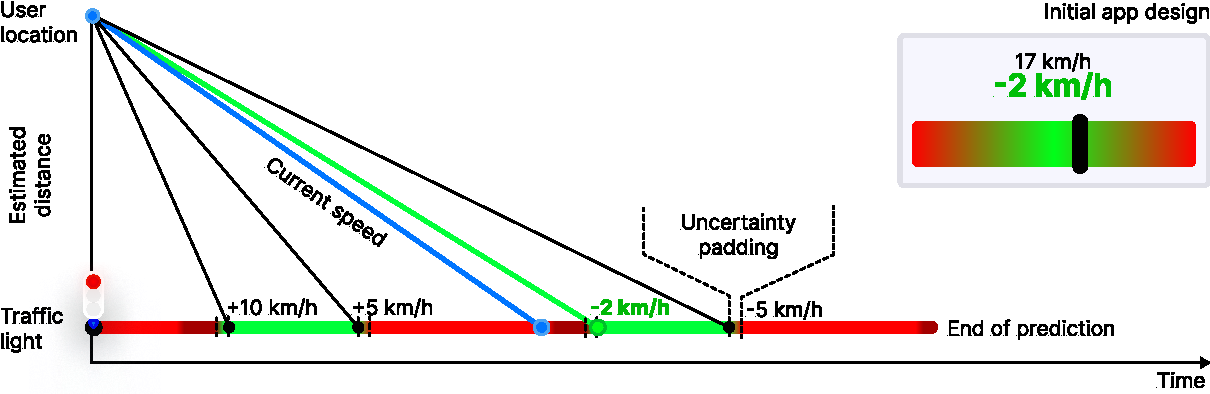
\includegraphics[width=\linewidth]{images/graph-based-speed-recommendation.pdf}
\caption{Simple speed recommendation algorithm used in initial tests.}
\label{fig:graph-based-speed-recommendation}
\end{figure}

Out of three user interface prototypes, one was selected for our deployment and test with users in Hamburg. Two user interfaces had shown in preliminary experiments to be less appropriate, and were thus not followed further: the target speed advisory and the multi-lane projection. We will briefly discuss the learnings from these approaches, as they have been crucial in shaping the final solution.

\Cref{fig:graph-based-speed-recommendation} illustrates our initial approach, the target speed advisory. In this approach, a text-based speed recommendation is provided to the user, accompanied by a static color-coded scale indicating alignment with the green phase. An ideal speed is determined based on a simple algorithm that incorporates the estimated traffic light distance and the traffic light's prediction. Based on the estimated speeds to arrive at the start or end of each predicted green phase, the closest target speed is selected to minimize the required speed adjustment. In case no speed adjustment is required to arrive at green, the currently driven speed is recommended. To incorporate prediction uncertainties in the speed advisory, an uncertainty padding is added to the predicted green phases. Finally, sanity checks are implemented to clamp the speed advisory to realistic speeds.

We experimented with this approach on a test track in Dresden. Two mobile traffic lights were set up on TU Dresden's campus, with a circular test track around the "Friedrich List" Faculty of Transport and Traffic Sciences. The traffic lights were equipped with fixed-time programs and positioned alongside a shared bike/footpath, where they would not interfere with automotive traffic. Based on this test setup, the following limitations were identified.

First, there was the issue of speed fluctuations and oscillation around the target speed. Presumably caused by GNSS inaccuracies and latencies in the recalculation of the GNSS speed, the difference between the target speed and the user's actual speed fluctuated from second to second, leading to a perceived lack of responsiveness. Since the user location (together with its speed) is maximally sampled once per second, we experienced stuttering recommendations instead of a smooth and continuous experience. This often resulted in excessive over- or under-compensation to reach the target speed, leading to an overall poor user experience. This issue could have been partially addressed by an external speed sensor or additional effort to incorporate the inertial smartphone sensors.

Due to similar reasons, the second issue of our approach was that it failed to consider acceleration inertia in the speed advisory calculation process. The calculation assumed that the user could instantly adjust to the recommended speed. However, the longer it took to match the speed recommendation, the greater the discrepancy became. Consequently, we felt a constant need to chase the speed recommendation, which contributed to a sense of dissatisfaction. Overall, our speed advisory model would have required a much more sophisticated motion estimation to address this problem.

Another difficulty related to modeling the cyclist's movement is considering the user's limits and capabilities. The speed advisory algorithm has to make assumptions about the user's physical abilities to accelerate and decelerate in a specific scenario. Similar to the work of Fickas et al. (2019) \cite{fickas_fast_2019}, we found this to be a major drawback, as users could be impeded by traffic or physically unable to meet the recommendations, leading to disappointment when a recommended speed can't be achieved. Even more frustration can occur with a false speed advisory after having spent additional energy to follow the recommended speed. While factors like incline in the path, surface quality, or the type of bike chosen (e-bike vs. regular bike) could be inferred with our route-based approach, not all real-world aspects perceived by the user can be adequately captured.

With our approach, there was also the risk of recommending a speed that conflicts with the user's intentions, as the system decides a speed for the user. However, the user's intention may be to ride comfortably while feeling pressured by the app to speed up. In situations where there is ambiguity, with some users opting to speed up while others prefer to slow down, the speed recommendation effectively works against one of these groups. We found no good ideas on how this challenge could be addressed.

Finally, there is the issue of prediction uncertainties. While Typaldos et al. (2023) \cite{typaldos_modified_2023} and Mahler et al. (2012) \cite{mahler_reducing_2012} have shown more advanced methods than our simple uncertainty padding method, the issue lies elsewhere: the explainability of a speed advisory. As the decision process happens in the background, it does not explain to the user why a specific speed was selected. This leads to situations where the speed advisory may overly slow down the user, focusing on a certainly green part of the prediction when the traffic light becomes green much earlier in the real world. The user could interpret this intended behavior as an imprecise speed advisory.

Overall, although some issues with out target speed approach can be attributed to the simplicity of our speed selection strategy and sensor processing, the main challenge lies in the limited explainability and the limited ability to capture user intentions with regard to the context's complexity. Smartphones cannot model the real-world situation more adequately than the cyclist himself. Projection-based methods are an obvious choice here, as they externalize the speed decision to the user.

\begin{figure}[t]
\centering
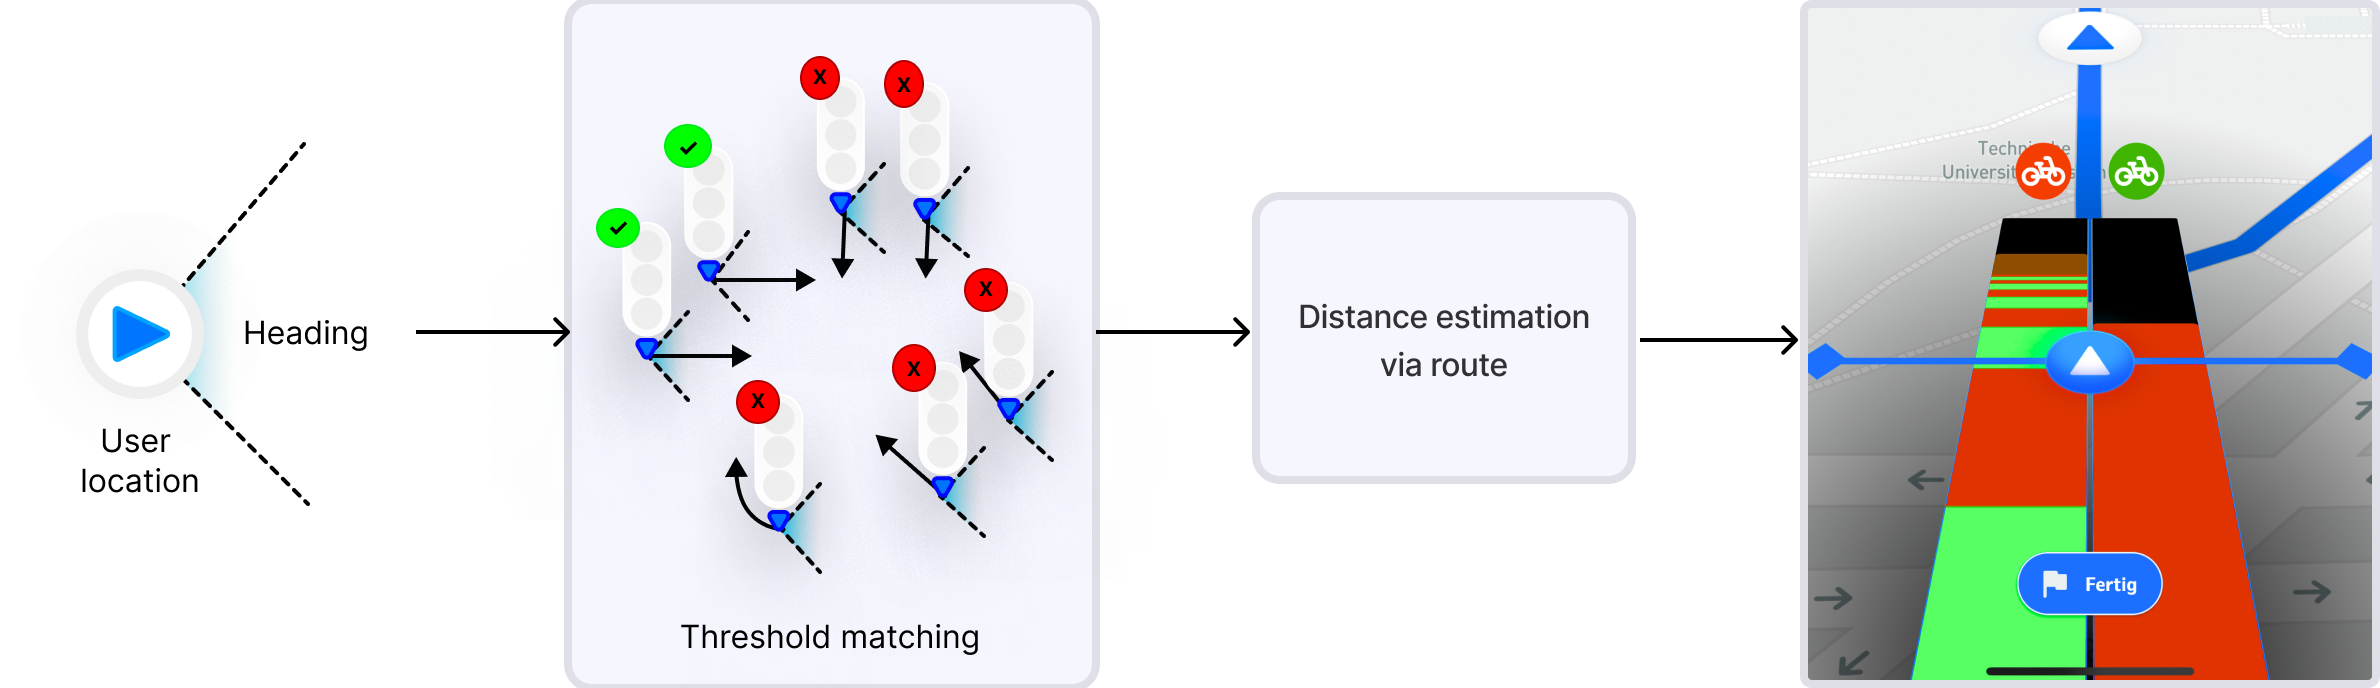
\includegraphics[width=\linewidth]{images/multi-lane-view.png}
\caption{Multi-lane matching and preliminary implementation of multi-lane speed recommendation.}
\label{fig:multi-lane-view}
\end{figure}

In another preliminary test, we experimented with the multi-lane projection method. This method solves the aforementioned modeling problem, as the user can flexibly choose between possible speeds. No speed advisory model is needed. Our approach involves displaying multiple parallel lanes for upcoming traffic lights, with the prediction projected onto these virtual lanes. The user's location and speed are rendered above these lanes, allowing the user to slow down or speed up to move the prediction underneath. As the intersection comes closer, the lane's end (stop line) moves toward the user. 

To implement this approach, we had to develop a multi-lane traffic light selection. Such a method was quickly established, looking up all signals on intersections along the route that match the route's direction. This process is illustrated in \Cref{fig:multi-lane-view}. As not one but multiple traffic lights were selected, this simplified the traffic light matching process drastically. The choice for the concrete traffic light is made by the user, not by a traffic light matching model. Thus, this method was initially very attractive.

However, the main drawback we experienced was the visualization's readability while riding. With multiple parallel signals being displayed, we had to mentally correlate the shown lanes with the real-world situation ahead and process predictions for multiple parallel lanes simultaneously. Although this finding is highly subjective, we found that a multi-lane visualization conveyed too much potential for user distraction, which we aimed to minimize.

Another more technical challenge lies in moving the predicted traffic light colors intuitively towards the signal, resembling a flow that the user can "hop on." A problem is choosing a suitable zoom scale for the prediction, such that users can differentiate when they will be "caught" or "run into" a red light. Similar to the initial color-coded scale, users also have to get used to the direction of movement that they can induce when they speed up or slow down. Again, we found that this approach could not be given to users in Hamburg, experiencing it as not well usable. Thus, after having experimented with various different changes to this user interface concept, we ultimately decided against this type of approach. 

Our decision against the multi-lane projection was also partially driven by the reason that we had found the third option substantially more promising: the speedometer projection. This visualization will be discussed in the next section.

\subsection{Combined Approach with Speedometer and Countdown}

The designed speedometer visualization aims to integrate the strengths and mitigate the weaknesses of both previous approaches. Unlike the multi-lane visualization, only one relevant traffic light is shown, reducing screen elements that need to be processed by the user. To find the specific traffic light toward which the user cycles, we utilize the developed traffic light matching approach from \Cref{ch:matching}. Simultaneously, no decision for a target speed is forced upon the user, diminishing almost all drawbacks seen with the target speed approach. The user can freely decide which speed should be chosen based on the displayed traffic light prediction. In this way, the presented type of visualization can be seen as a compromise between the target speed advisory and multi-lane projection.

\begin{figure}[t]
\centering
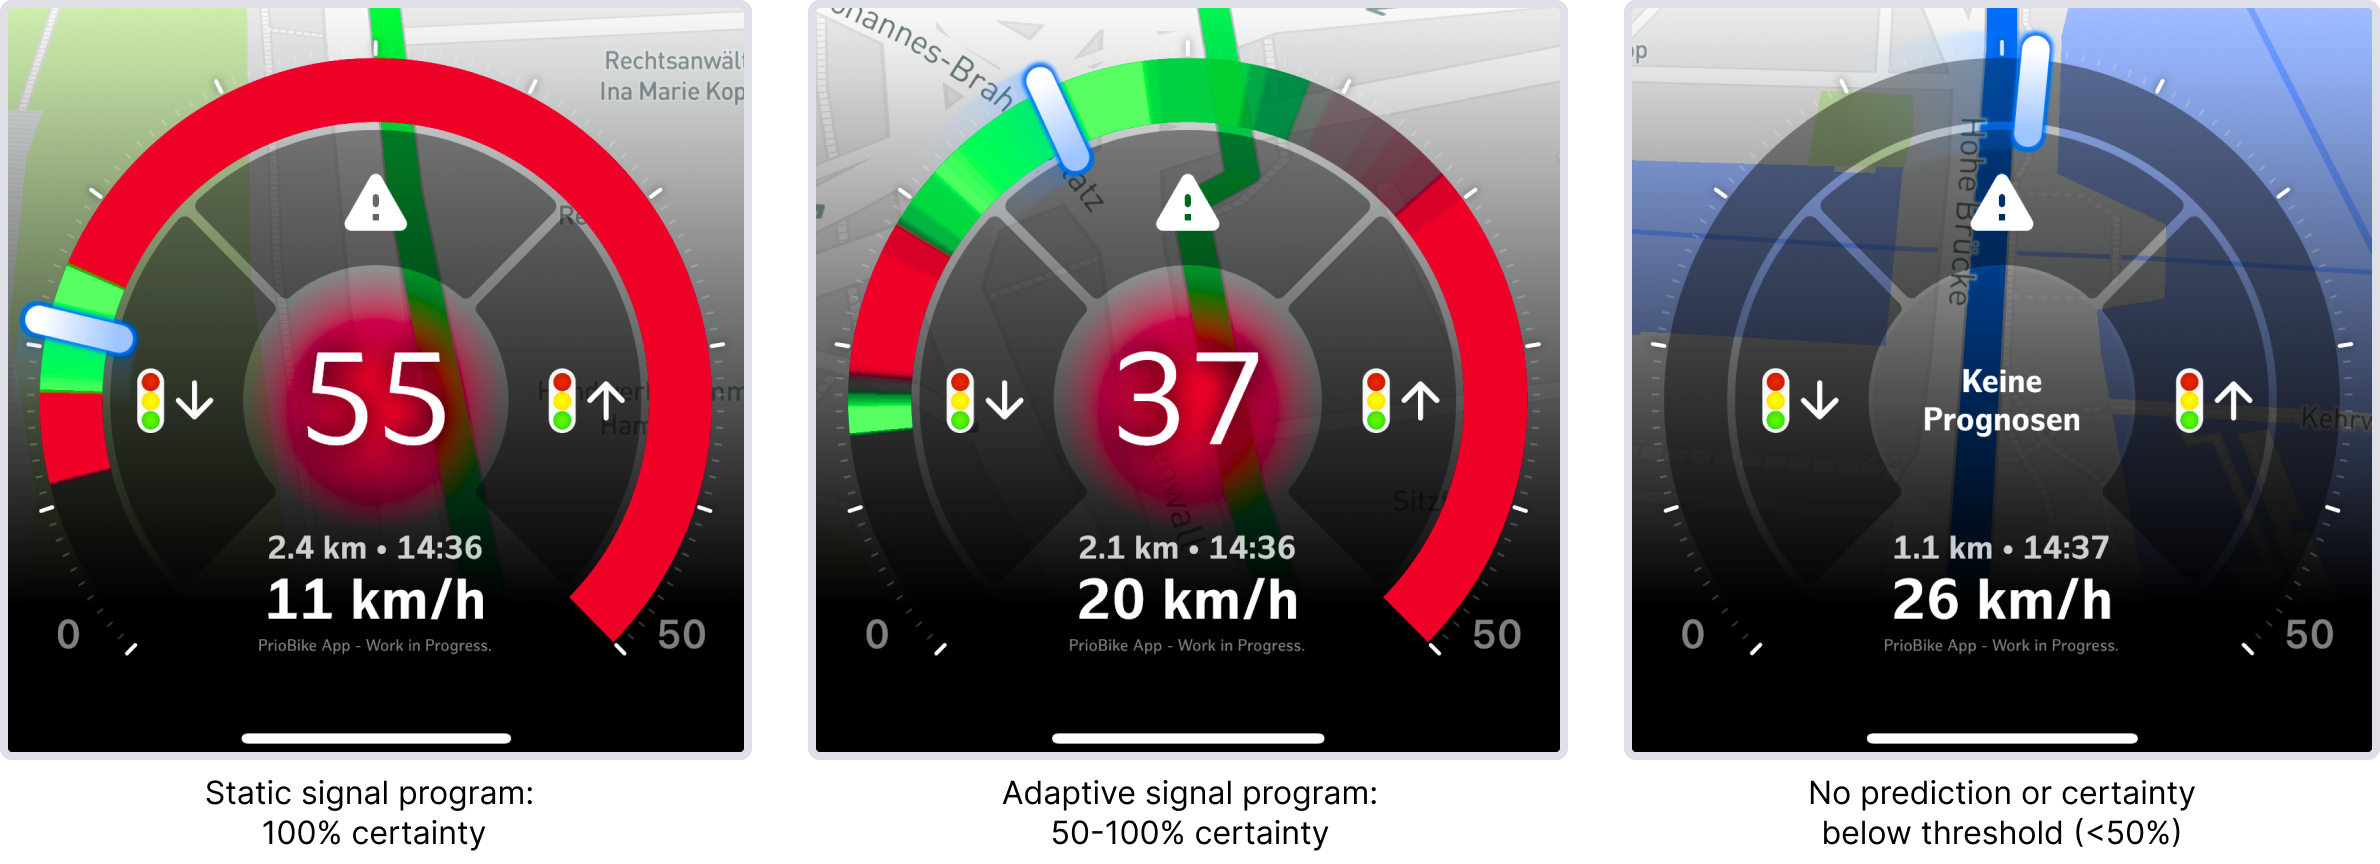
\includegraphics[width=\linewidth]{images/speedometer-adaptions.png}
\caption{Final speed recommendation concept and adaption mechanisms for varying prediction quality.}
\label{fig:speedometer-adaptions}
\end{figure}

To address prediction uncertainties, the speedometer incorporates a mapping of these uncertainties by adjusting the opacity of the green or red colors. This adaption is also highlighted in \Cref{fig:speedometer-adaptions}, and conveys certain and uncertain parts of the prediction to the user. 

In addition, to avoid users adapting to a poor traffic light prediction, the speed advisory is only displayed if the prediction quality is above 50\%. This quality threshold is set quite low compared to other works \cite{protschky_extensive_2014, protschky_adaptive_2014}, assuming that the remaining prediction uncertainty above 50\% quality is sufficiently conveyable through the blurred prediction regions. The defined threshold can surely be optimized further based on the demand for more reliable or more available speed advisories. 

To provide additional information, especially when standing at an intersection, a traffic light countdown has been included at the center of the speedometer. Like in related works \cite{stahlmann_exploring_2018, sokolov_effects_2018}, this countdown is hidden 5 seconds before the traffic light switches. However, the countdown is also hidden if the prediction quality is below the defined quality threshold. In this way, users are demotivated to overly trust an inaccurate countdown and potentially cause accidents.

Two more enhancements were implemented to account for smartphone GNSS accuracy and frequency, potentially varying between device vendors. First, to compensate for fluctuations in the measured GNSS speed, a smooth animation is applied to the speedometer needle. In this way, we establish a sense of responsiveness even in the presence of low-frequency GNSS sampling. Finally, additional buttons are given to switch to the next or previous traffic lights just in case the position cannot be accurately associated. This option is given in addition to the automated snapping method developed in \Cref{ch:routing}, which determines whenever a traffic light is overshot by the GNSS position and keeps the user associated with it.

Concluding this section, three identified visualization methods have been investigated and thoroughly tested. Out of the three options, the speedometer visualization is considered the best option. The user interface is designed to account for different situations, such as bad predictions or poor GNSS accuracy. Automated self-adaption of the user interface is a large aspect here, so no active interaction during the ride is required in most instances.

\subsection{Routing-Enhanced Speed Advisory}

\begin{figure}[t]
\centering
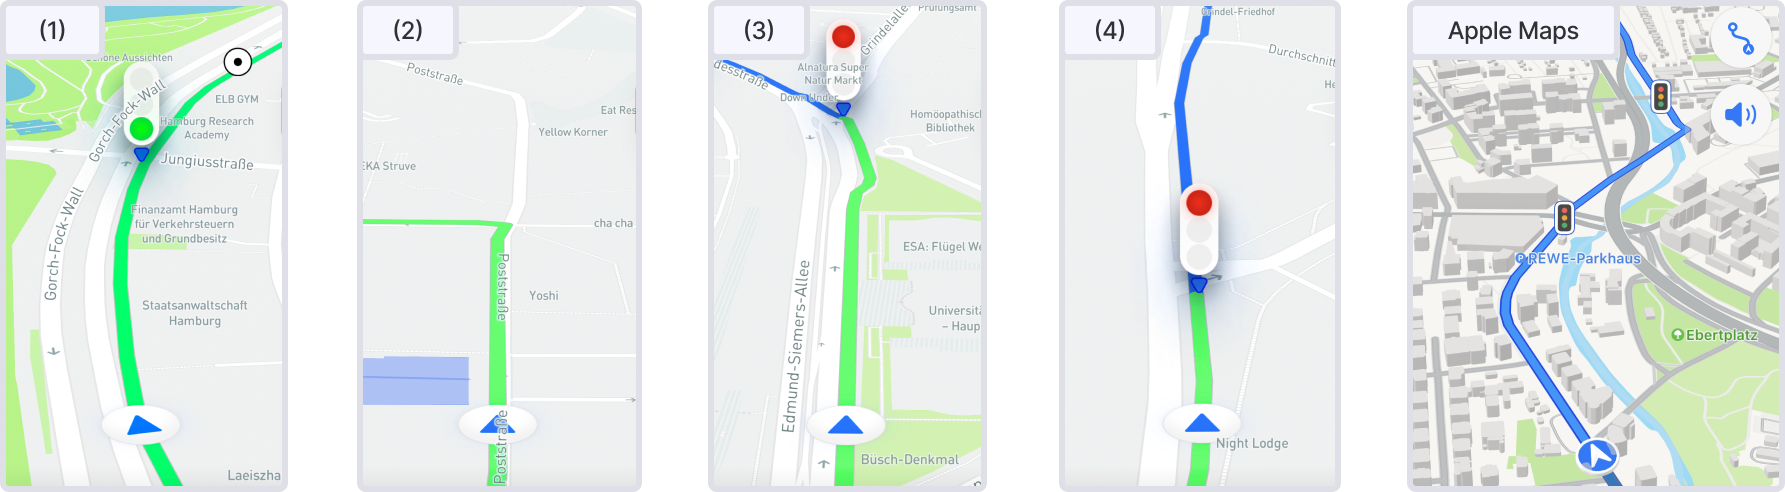
\includegraphics[width=\linewidth]{images/camera-controller-1.png}
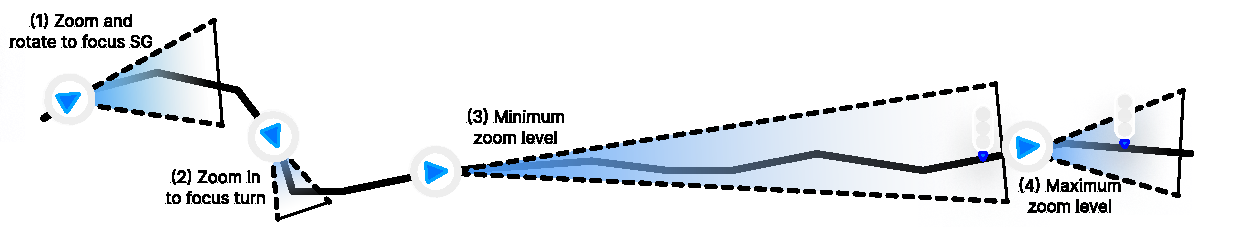
\includegraphics[width=\linewidth]{images/camera-controller-2.pdf}
\caption{Dynamic camera adaption in different scenarios.}
\label{fig:camera-controller}
\end{figure}

The integrated routing is utilized to enhance two aspects of the speed advisory. First, the traffic light for which a speed advisory is displayed can be shown along the route on the smartphone's display. The goal is to avoid confusion when a false traffic light is selected. Secondly, the route is utilized to convey for which parts of the planned trajectory a speed advisory will be given. This additional information is intended to help users plan routes with higher speed advisory coverage, as not all intersections are connected to the system. In addition, intersections not sending data are shown, so that a user understands why they may not receive a speed advisory at the moment, enhancing the overall explainability.

Displaying the upcoming traffic light on the map is quite trivial -- no further consideration is needed here. However, often, the currently selected traffic light or next turn is out of view when the camera strictly follows the user's position and heading at a fixed height. To improve this aspect of responsiveness and avoid users attempting to pan/zoom during bike rides, the map's camera is automatically adjusted to focus on traffic lights and close turns. This feature was adopted from Apple Maps, as seen in \Cref{fig:camera-controller}, which also incorporates the route's curvature to suitably orient the map's camera.

The specific process is as follows. During a ride, the app continuously checks if the user is approaching a traffic light by examining the route segments from the user's location. A turn is detected when a route segment is found that deviates at least 15° from the user's measured heading. As the user approaches a turn or traffic light, the camera automatically zooms in to focus on the intersection, making it easier for users to locate a path entry or identify a corresponding signal. Additionally, the camera rotates slightly (up to a maximum of 20°) away from the user to ensure that the traffic lights remain within the view frustum. These threshold values have been determined empirically through extensive real-world testing. To prevent excessive zooming, the camera operates within specified maximum and minimum zoom levels, avoiding zooming too far out or too far in.

In addition to the camera controller, the prediction availability is also mapped across the route. As seen in \Cref{fig:camera-controller}, route segments with speed advisory are colored green, indicating these segments provide a "green wave." 

\begin{figure}[t]
\centering
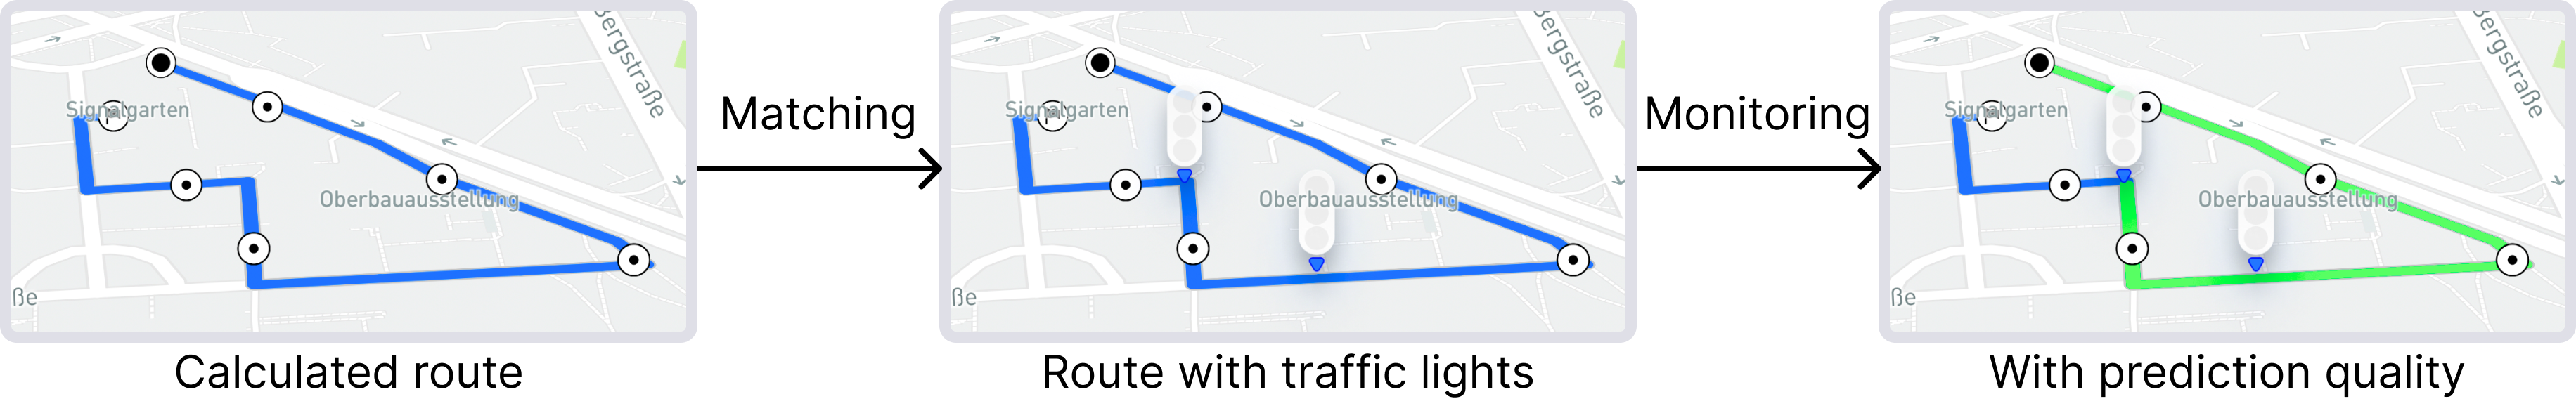
\includegraphics[width=\linewidth]{images/routing-process-quality-mapping.png}
\caption{Visualization of traffic light groups and prediction quality along the calculated route.}
\label{fig:routing-process-quality-mapping}
\end{figure}

To match the prediction qualities onto the route, two steps illustrated in \Cref{fig:routing-process-quality-mapping} are performed: First, the traffic lights are matched along the route, using the approach developed in \Cref{ch:matching}. Afterward, the obtained traffic light IDs along the route are utilized to fetch and map the prediction qualities generated by our prediction monitoring. Finally, the route is colorized with respect to the prediction quality. No prediction means the route is not colored green. A prediction with less than 50\% quality is also not displayed as green since no speed advisory is activated. Upwards, the color is interpolated between the default route color (50\% quality) and green (100\% quality).

In summary, the smartphone application not only displays a bare route geometry as in other navigation applications. It also utilizes the route to enhance the overall speed advisory, conveying a relation to advised traffic lights and telling users which route sections will be covered by a speed advisory. In this way, the explainability of the overall application is enhanced, with the goal of avoiding frustration during rides when no speed advisory can be given. The speed advisory also operates together with two other application services designed in \Cref{ch:routing}: automated rerouting and route-based GNSS error correction.

\subsection{Final Application Architecture and Design}

Now that we have looked at the many details of the speed recommendation, it is vital to take another look at the overall picture. In this way, we gain a thorough understanding of how all the designed components from the four discussed chapters work together to create the final Green Light Optimal Speed Advisory system for bikes. We will also briefly go over additional components for traffic prediction, geocoding, and map layers that are used to provide convenience features for pathfinding.

\begin{figure}[t]
\caption{Final application infrastructure.}\label{fig:architecture}
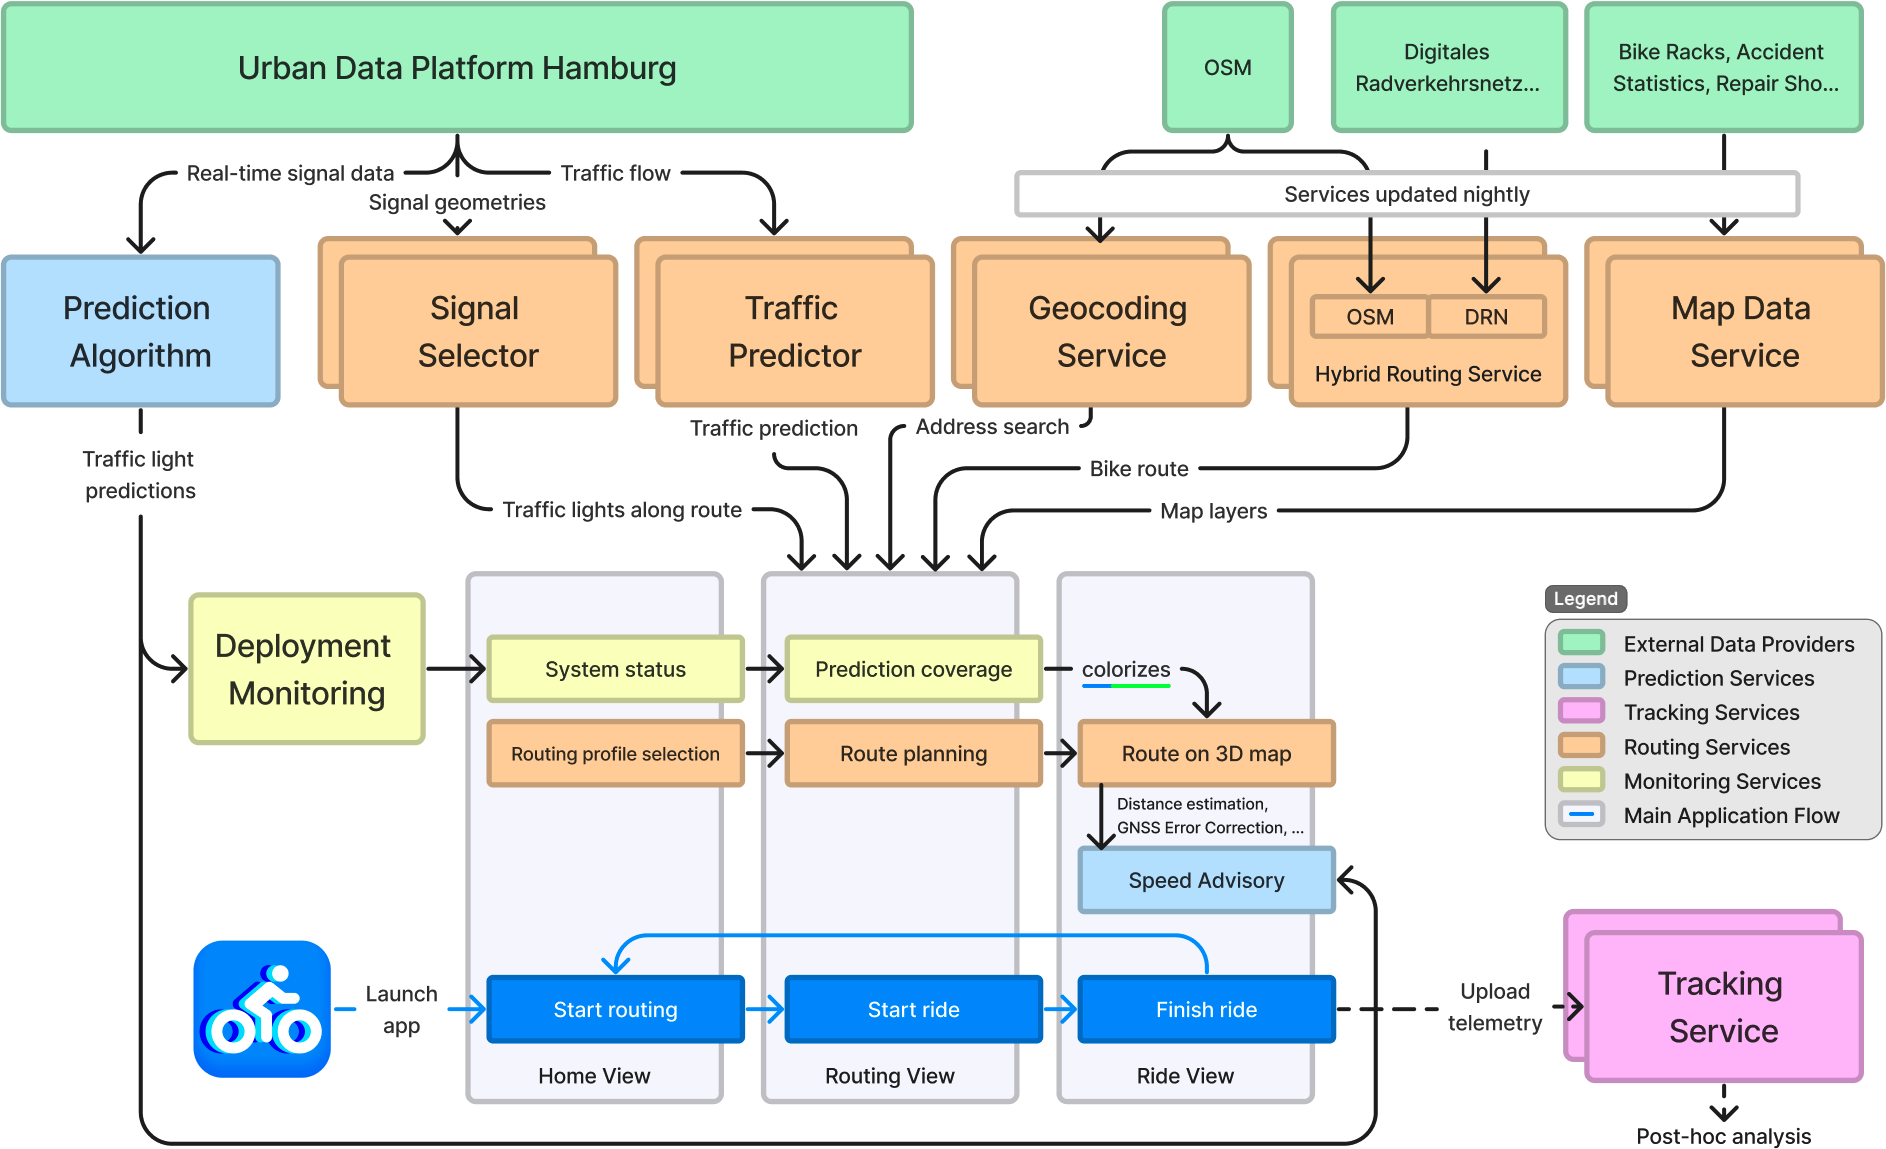
\includegraphics[width=\linewidth]{images/architecture.png}
\end{figure}

As seen in \Cref{fig:architecture}, the main application flow is divided into three views. The home view, serving as an entry point after opening the app, is intended to display the current data availability upfront. With the information fetched from the prediction service monitoring, users are directly informed about potential data outages. These can occur spontaneously, as we have seen in \Cref{ch:prediction}. A modification of the routing profile is also possible in the home view.

\begin{figure}[t]
\caption{The final mobile application distributed to users.}\label{fig:app}
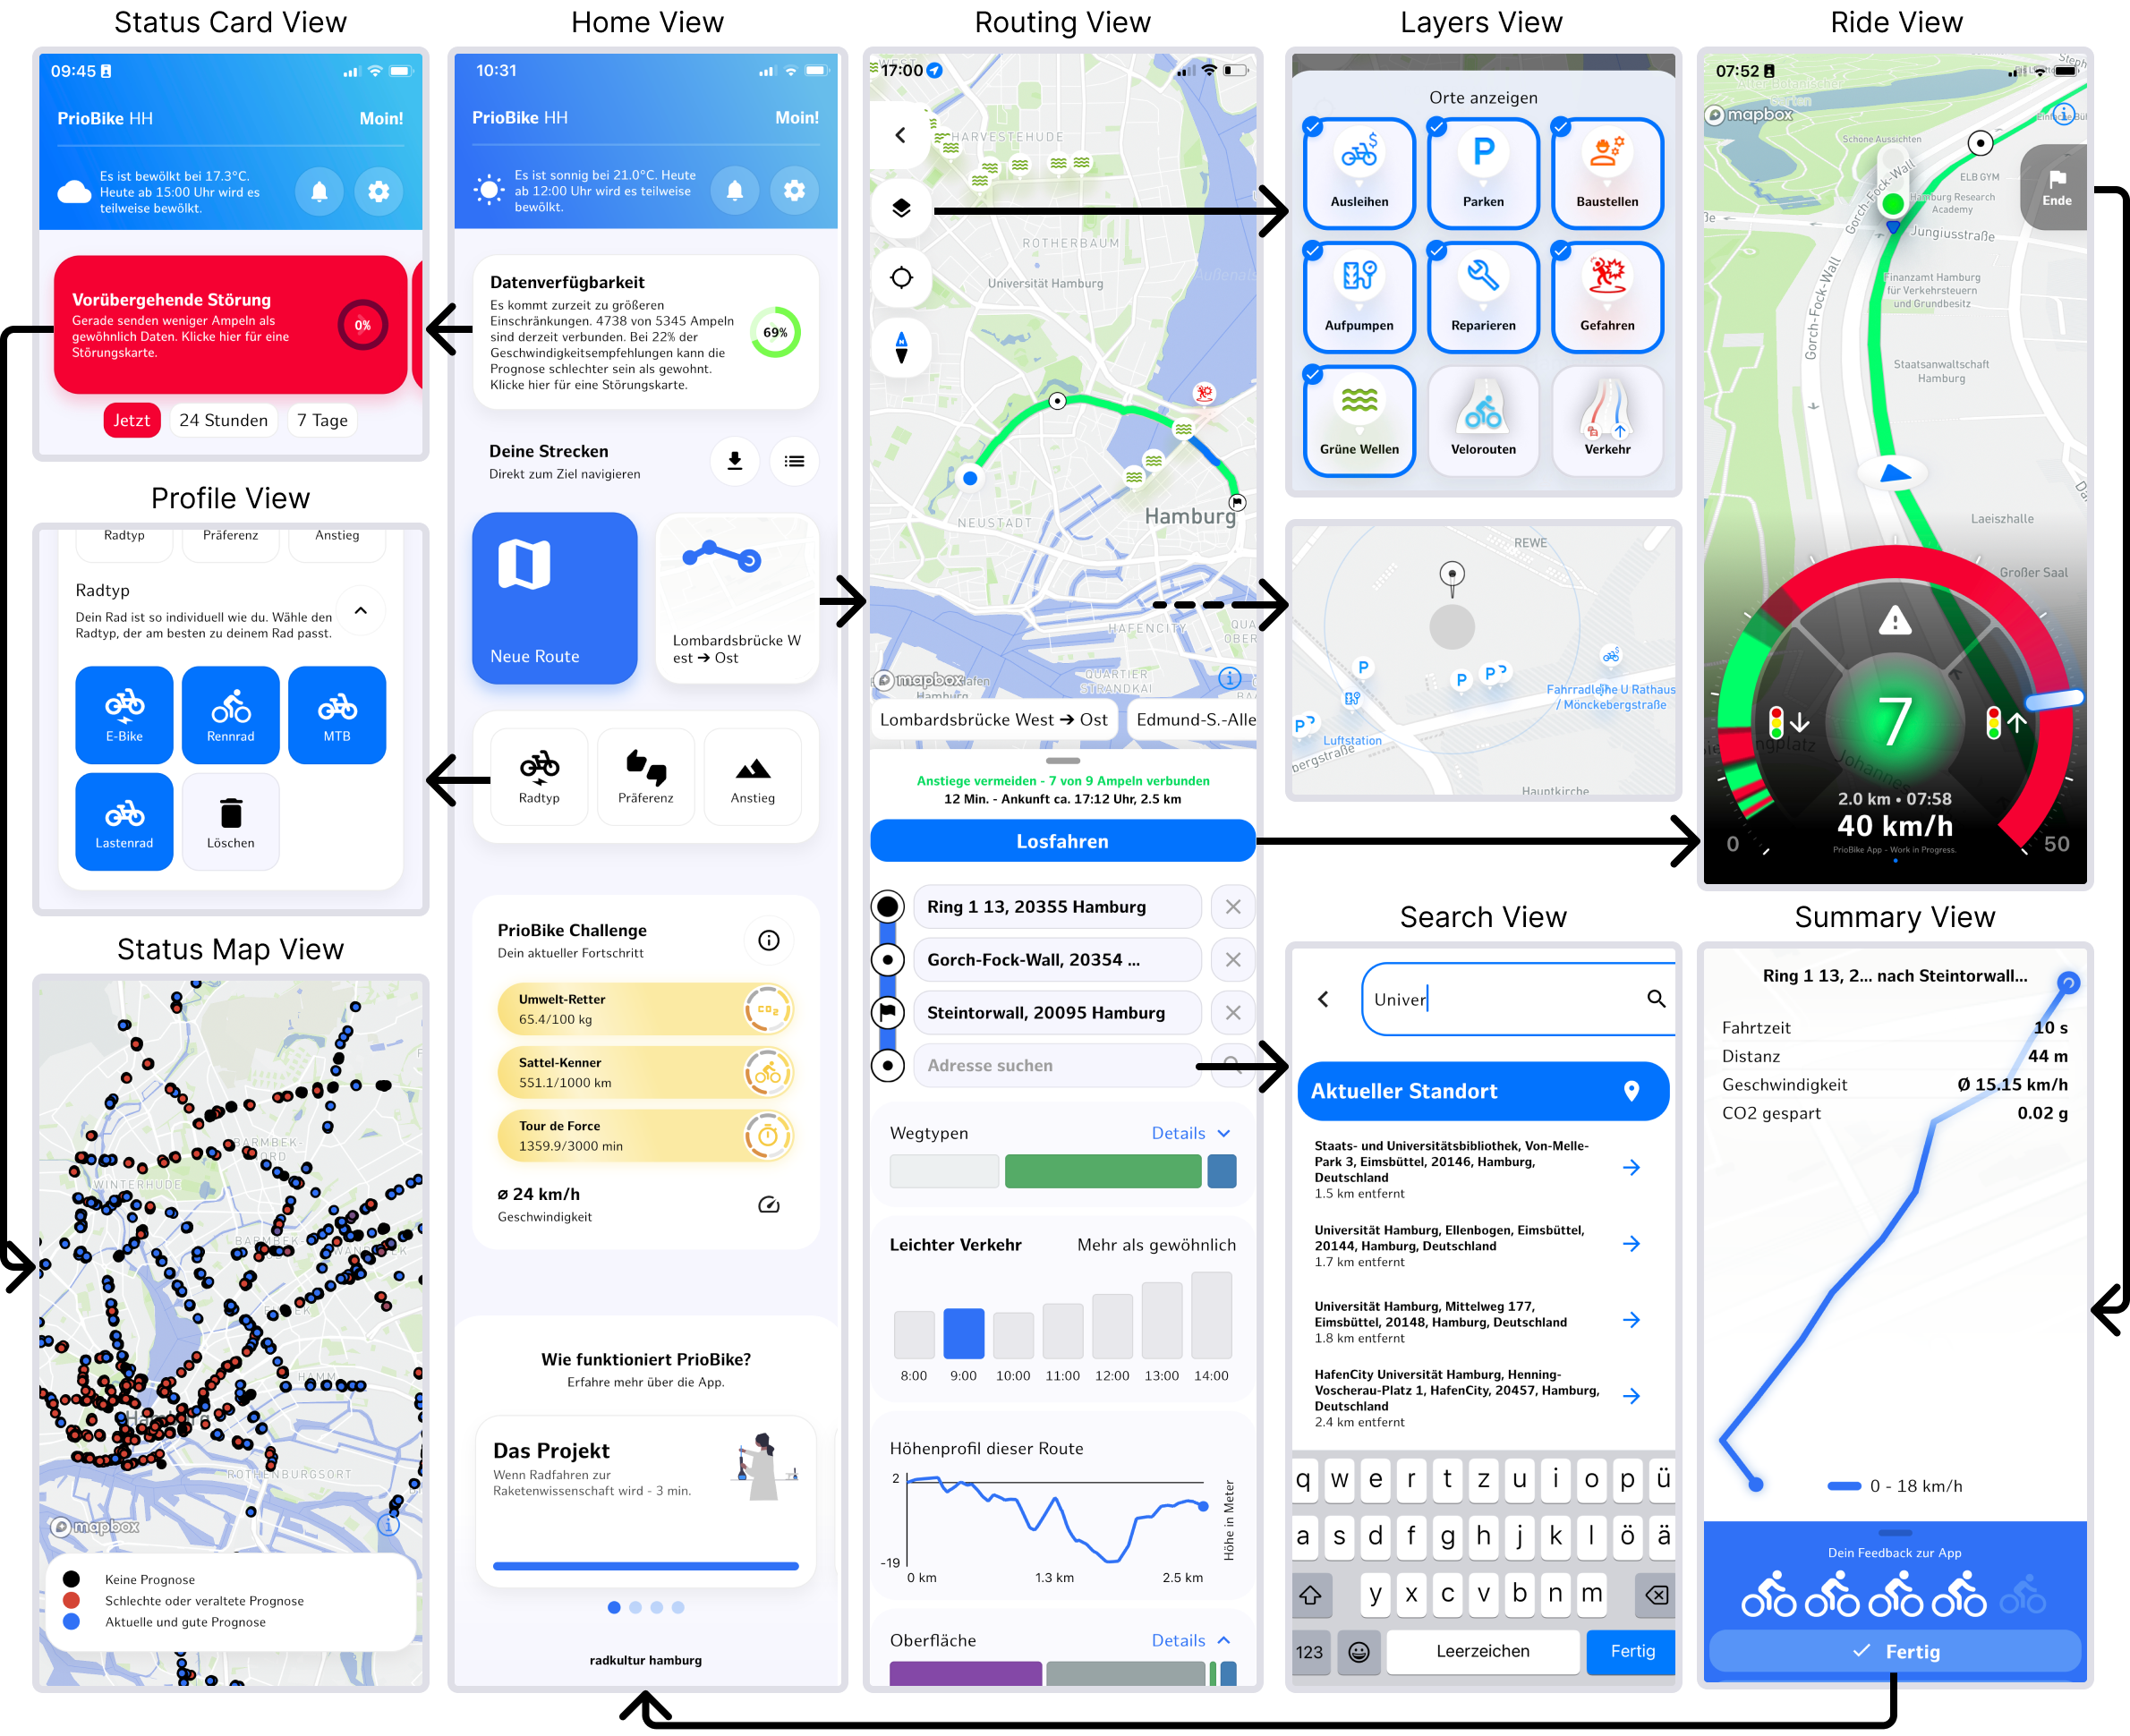
\includegraphics[width=\linewidth]{images/app.png}
\end{figure}

Afterward, users transition to the routing view. Here, users may select waypoints to generate a route, similar to other navigation apps like Google Maps, Komoot, or Strava. Along the bike route generated with the DRN routing from \Cref{ch:routing}, traffic lights are matched through the service from \Cref{ch:matching}. The route's prediction coverage is fetched and displayed to the user. Additional path metadata from our routing is also displayed, including path inclination, to enable a more informed routing decision. How this looks on the smartphone's screen is presented in \Cref{fig:app}. In the routing view, three more convenience services are added: a simple traffic predictor, a geocoding service, and a map data service.

The traffic flow algorithm predicts traffic density in Hamburg by assigning weights to road paths based on congestion levels, calculating a normalized score relative to the path's length within the road network. Afterward, the normalized scores are summed to generate an overall traffic flow factor, ranging from 0 (complete congestion) to 1 (free flow). At its foundation, the traffic flow prediction algorithm utilizes open floating car data from INRIX, given through the "Verkehrslage Hamburg" dataset that is updated every 5 minutes.

To find addresses, a geocoding service is also added to the deployment. Initially, Nominatim was chosen as a geocoding service based on OpenStreetMap. However, the solution has shown limitations when it comes to supporting partial queries, such as searching for "University" using "Univers," and its response time was perceived as too slow (often more than 2 seconds) during preliminary tests. Therefore, we switched to Photon (by Komoot) as an alternative open-source solution that supports partial queries and provides faster query execution.

Bike-specific points of interest, such as air pumps, bike parking spots, repair shops, and rental stations, are added through various open datasets from the city of Hamburg. The geodata is processed and distributed on a nightly basis, similar to the routing engine. Bike accident hotspots are also extracted from the Unfallatlas\footnote{\url{https://unfallatlas.statistikportal.de/}} dataset and clustered. Afterward, they can be fetched through a map data service and displayed in the mobile application.

Having started the ride, the user transitions to the ride view. Here, the speed advisory is displayed together with the calculated route. Based on the estimated route-based distance to the upcoming (preselected) traffic light, the traffic light prediction is mapped over the speedometer and displayed as a countdown. The prediction is obtained during the ride by subscribing to the MQTT topic for the specific traffic light ID on which new predictions are published. Other route-based services for camera adaption and GNSS error correction run in the background to provide smooth and stable navigation. As users deviate from the route, the developed approach for rerouting ensures that a route is recalculated as needed.

Finally, a tracking service is implemented that obtains ride statistics from users. The collected telemetry data is used to conduct post-hoc analyses on the actual impact of bike-GLOSA on ride behavior.

\begin{Summary}[Summary of Methods]
The speed advisory application designed in this work distinguishes itself from previous work by choosing an entirely route-based approach. After calculating an accurate bike route through the integrated wayfinding tools and the developed bike routing from \Cref{ch:routing}, traffic lights are automatically matched as discussed in \Cref{ch:matching}. Through the route-based distance-to-signal estimation and the prediction methods from \Cref{ch:prediction}, the app can calculate a speed advisory along the selected route. The speed advisory approaches target speed recommendation and multi-lane projection were tested preliminarily, but not further explored. These are likely not a good option for cyclist applications of GLOSA. The chosen speedometer approach was optimized to include a responsive countdown timer, and a camera movement controller that establishes a visual relation to the recommeded traffic light. In its final integration, the mobile application utilizes a few more briefly discussed auxiliary services to enhance the informativeness of routing, such as displaying the speed advisory coverage along the selected route. These concepts aim at enhancing the app's suitability for everyday tasks as much as possible. 
\end{Summary}

\section{Results}

Our developed concept provides the foundation for our final evaluation: a large-scale field test in Hamburg, in which users try to integrate the application into their daily life. This evaluation approach contrasts previous bike-related studies, which have been conducted in test-track or simulation environments. Instead, residents of Hamburg were able to voluntarily register for the test, download the app, and independently use it according to their needs, without further instructions. This testing approach includes the freedom for users to choose a route through the city, along which various connected and unconnected traffic lights, both well and poorly predicted, may be encountered. The experiment's duration is also much larger, as our study spans across March 2023 to December 2023, coinciding with the beta stage of our developed app.

Our upscaled real-world test aims to capture the impact of speed recommendations on cyclists as realistically as possible. However, the increase in study complexity also introduces additional challenges, particularly in data analysis. For example, we can no longer assume that users will only choose predefined routes for speed advisory, containing traffic lights that are also suitable for prediction. In such a complex setting with various possible routes, traffic situations, types of devices, users and attitudes, the main goal is to overcome challenges in analysis while deriving as many reliable insights as possible. 

A twofold study design is chosen. Initially, a user survey through our app is conducted, in which our test users can voluntarily participate. This yields demographic statistics about our user base, standardized SUS ratings for usability, and more detailed individual feedback on both positive and areas for improvement. Subsequently, we transition to a quantitative analysis. By studying recorded interactions with the user interface, we examine how often users physically interact with the smartphone and explore ways to further reduce potentially hazardous interactions during cycling.

The core of our quantitative evaluation focuses on the impact of speed advisories on intersection approaches, calculating multiple impact metrics. To distinguish between well-utilized and poorly-utilized speed advisories, we measure the user's adherence to the recommended green phase(s). This allows us to categorize three cases: intersection approaches without speed advisories, those with adhered-to speed advisories, and those where the speed advisory was not utilized for various reasons. With this differentiation and the recorded tracks, we calculate the influence on intersection approach speed, increase or decrease in energy expenditure, as well as the number of stops and stop duration. Finally, we cross-validate our results and discuss the main findings, setting them in relation to previous studies.

\subsection{Collected Data}

\begin{figure}[t]
\caption{Collected ratings, tracks, and completed survey answers over time.}\label{fig:app-usage-over-time}
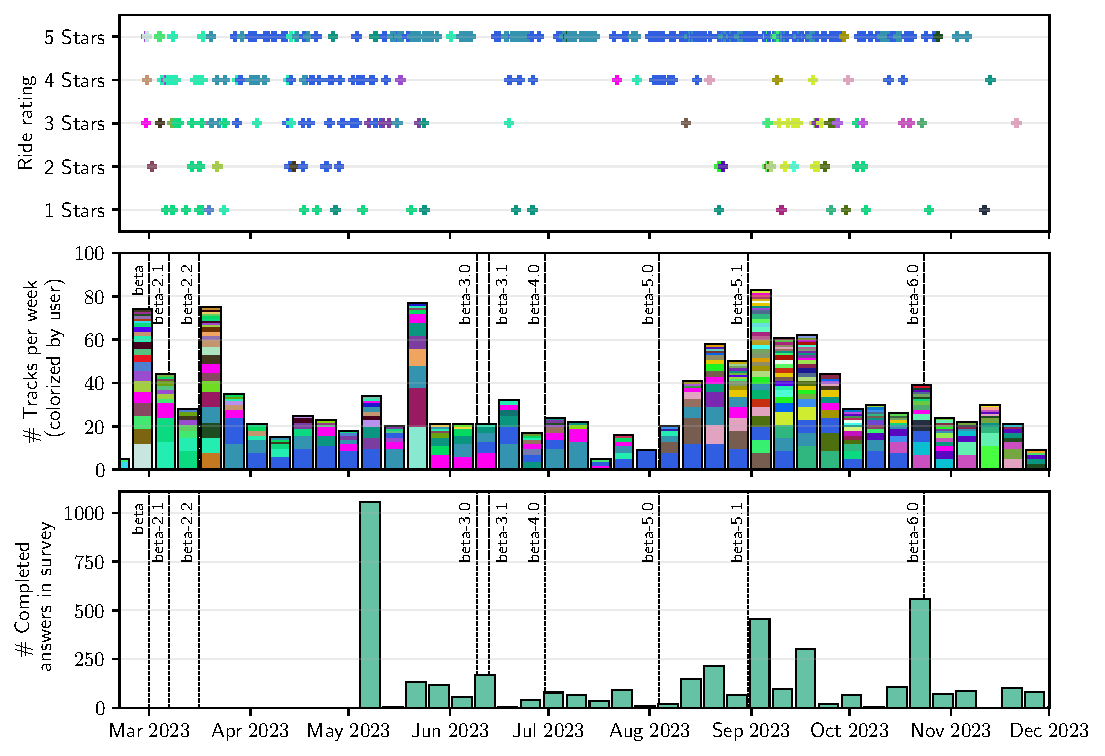
\includegraphics[width=\linewidth]{images/app-usage-over-time.pdf}
\end{figure}

Throughout the recorded time span from March 2023 to December 2023, as highlighted in \Cref{fig:app-usage-over-time}, various users have downloaded and tested the app. Based on statistics obtained from the Google Play console and AppStore Connect on February 5, 2023, the mobile application was installed on at least 130 Android and 178 iOS devices. Among these devices, 126 distinct user IDs recorded tracks in Hamburg. A user id is generated on every fresh installation of the mobile app, meaning that only a part of the users who installed the app also used it on real bike rides in Hamburg. Development devices and users who tested the application only on test setups in Dresden are likely the main reason for this difference.

Throughout the testing period, 1655 tracks were recorded, resulting in approximately three weeks of continuous driving data. From these tracks, 325 were filtered out during preprocessing, as they contained fewer than 30 GNSS samples and were considered too short to provide reliable measurements. On some occasions, the GNSS data could not be decoded properly due to an intermittent implementation error. However, these occasions represent a small minority in the collected tracks.

Clearly visible in \Cref{fig:app-usage-over-time} is that the frequency of rides has not been continuous over the months, but tracks were instead collected in "bulks." This can be explained by our strategy to fan out the test version to new users. While initial beta test versions were distributed in a closed beta schema on request via email, later versions were opened to the public with a download link. Simultaneously, there were some occasions on which the app test was advertised on social media platforms, leading to an increase in testers around September 2023. This increase persisted until the winter, in which it is expected that much fewer cyclists test the app. During December 2023, only a handful of users did drive with the app, denoting the end of our data collection period. 

After a track was driven, users were able to give their opinion on the ride, from 1 to 5 stars. As shown in \Cref{fig:app-usage-over-time}, a wide variety of ratings were given. Users who stuck to the app after initial tests were apparently very satisfied, as seen by the repeated 5-star ratings by the same user IDs. In general, there seem to be a few highly engaged users with the IDs \#305ee0 (201 tracks), \#3494b0 (150 tracks), \#ff00f0 (91 tracks), and \#0a9580 (59 tracks). The remaining 122 user IDs have collected fewer tracks, including 35 user IDs that only uploaded one track. The median number of tracks per user lies at 3.5 (IQR: 8.75), indicating a high diversity in users but also a low rate of users sticking to the app. Potential reasons will be investigated later in more detail, based on the collected user opinions.

\begin{figure}[t]
\caption{Spatial coverage of recorded tracks and collected surveys by postal areas.}\label{fig:app-spatial-distribution}
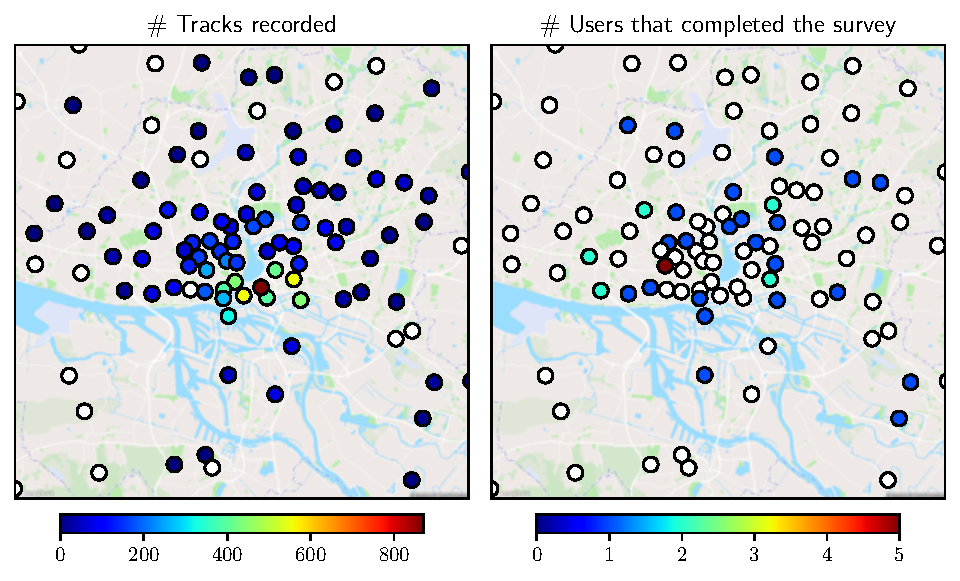
\includegraphics[width=\linewidth]{images/app-spatial-distribution.pdf}
\end{figure}

As seen in \Cref{fig:app-spatial-distribution}, tracks were recorded in a large variety of areas throughout the city, although more central districts are covered most. This is expected, as tracks tend to intersect in the center region. Also shown is the spatial coverage of 40 users who completed all questions in the survey, representing a 31.7\% participation rate of all distinct installations on devices.

Based on this subset of users, the median study age is 37 years (IQR: 22.5 years), ranging from 18 to 65 years. While we have a large age diversity, respondents report mainly to be male (34), with female (5) and diverse (1) subjects representing a minority. Thirty of our testers reported being employed, with eight testers declaring other occupations such as being a student (3), self-employed (2), apprentice (1), or pensioner (2).

The majority of our survey participants are already familiar with navigation apps. The main favorites seem to be Komoot (17) and Google Maps (13), besides other apps such as Bike Citizens (2). Among other responses, two users also declared our app "PrioBike" their favorite bike navigation app. 

A more diverse landscape can be seen with the preferred bike type. Users reported to use a city bike (19), trekking bike (10), mountain bike (6), racing bike (5), cargo bike (4). One user reported using a commuter bike, a custom kind of gravel or racing bike. Besides these likely non-motorized bike types, 12 users also reported using an e-bike. Among these, six users reported their e-bike to be offroad-capable. 

All respondents of the survey considered themselves to be experienced cyclists -- none selected the option "inexperienced." When asked which type of activity users would prefer a car over a bike, 12 respondents reported using a car for shopping activities. Also, 12 replies were related to free time activities or vacations, while eight answers considered daily work commutes as a reason to prefer a car. Transporting larger goods such as furniture or general errands (6) or longer distances (4) play a role in the decision as well. 

Based on the survey answers, a noticeable part of respondents seem to strongly advocate for cycling, and only utilize a car whenever no other option is present. Three subjects responded they avoid a car in any situation. Thus, we generally observe that many users who responded to our survey are already highly engaged in bike riding: 26 users use their bike on a daily basis, 12 users occasionally during the week, and two users sometimes on a monthly basis. These aspects will be considered when interpreting individual feedback, but also give insights into the representativeness of the collected tracks.

\subsection{System Usability Scale and User Opinions}



- SUS Score
- Number of completed scores: 33
- Median: 72.5 (IQR: 15.0), Min: 42.5, Max: 95.0

\begin{figure}[t]
\caption{Route fit for bike paths and planning intuitiveness.}\label{fig:route-fit-bike-paths}
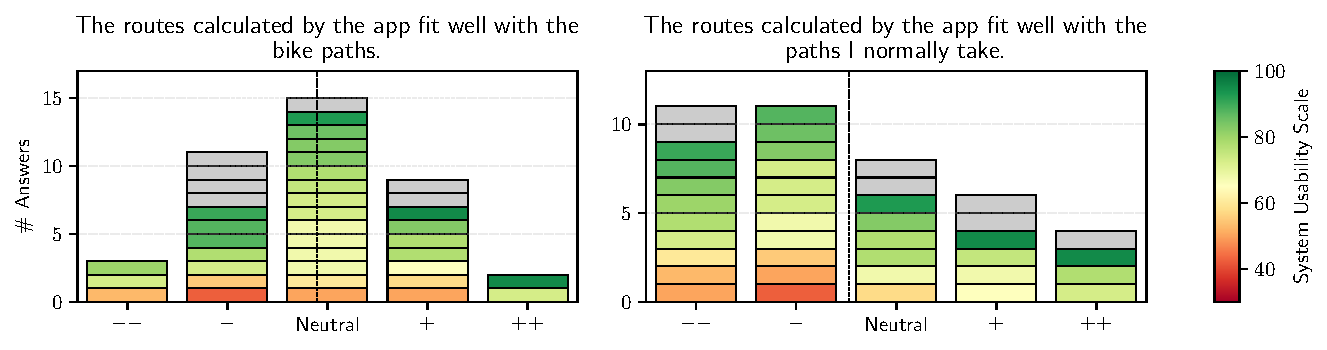
\includegraphics[width=\linewidth]{images/app-usability-questions-route-fit-bike-paths.pdf}
\\
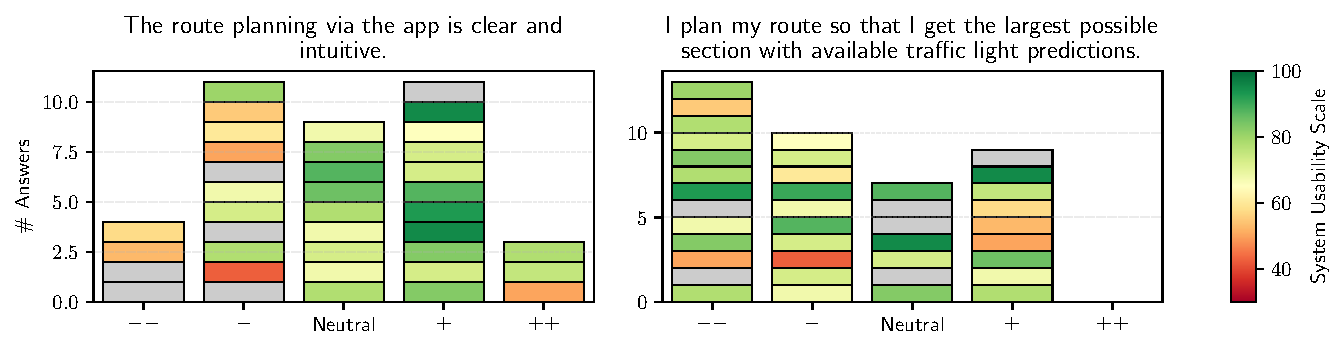
\includegraphics[width=\linewidth]{images/app-usability-questions-route-planning-intuitiveness.pdf}
\end{figure}

\begin{figure}[t]
\caption{Route personalization preferences and adaptation.}\label{fig:route-personalization}
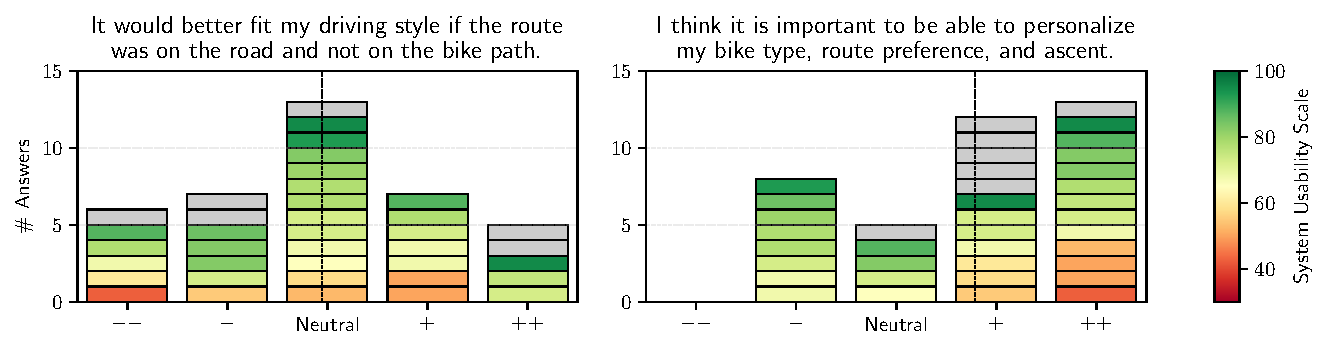
\includegraphics[width=\linewidth]{images/app-usability-questions-route-personalization.pdf}
\\
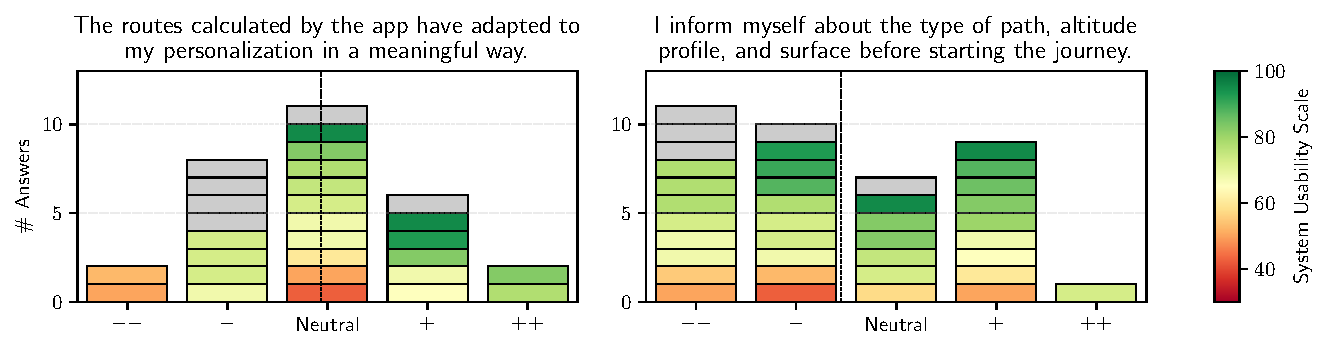
\includegraphics[width=\linewidth]{images/app-usability-questions-route-personalization-adaptation.pdf}
\end{figure}

\begin{figure}[t]
\caption{Speed advisory satisfaction, reliability, and utility.}\label{fig:speed-recommendations-satisfaction}
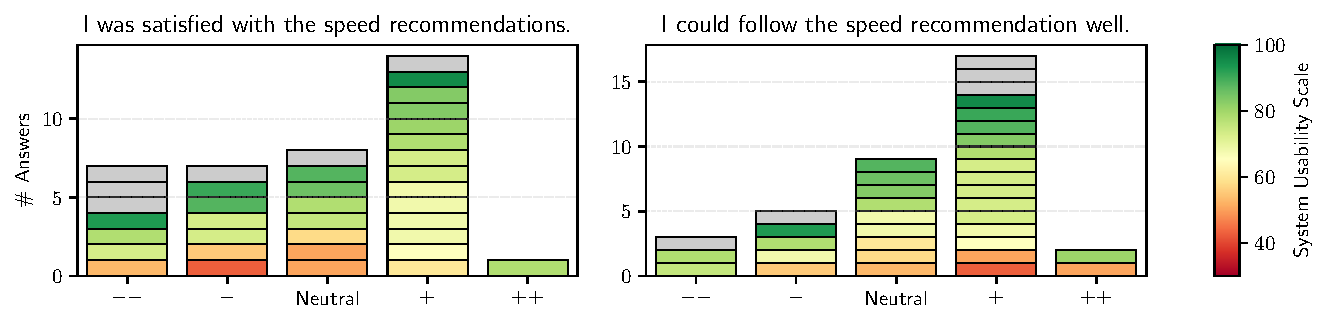
\includegraphics[width=\linewidth]{images/app-usability-questions-speed-recommendations-satisfaction.pdf}
\\
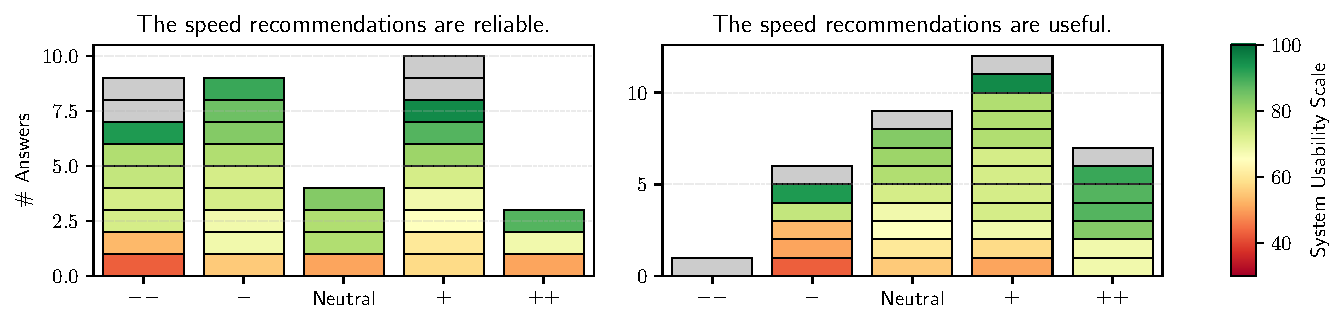
\includegraphics[width=\linewidth]{images/app-usability-questions-speed-recommendations-reliability.pdf}
\end{figure}
          

\begin{figure}[t]
\caption{Perceived impact on waiting time and safety}\label{fig:waiting-time-at-traffic-lights}
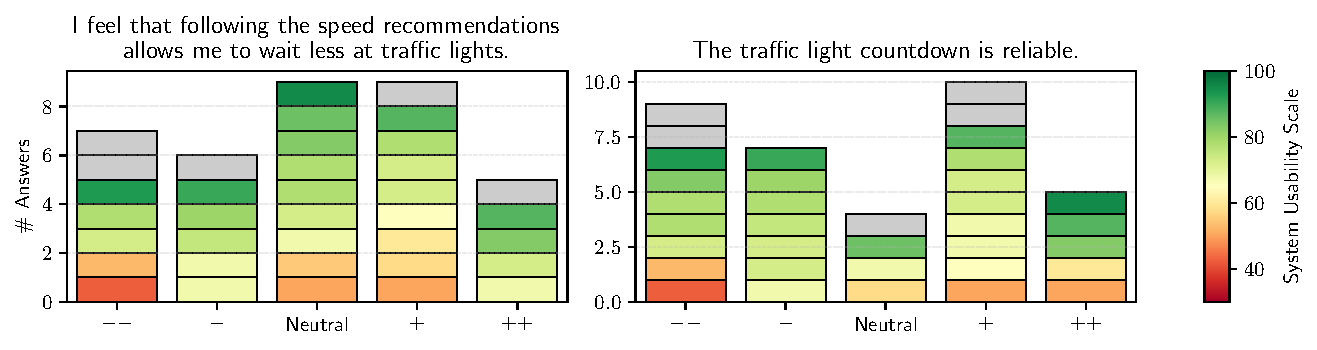
\includegraphics[width=\linewidth]{images/app-usability-questions-waiting-time-at-traffic-lights.pdf} 
\\
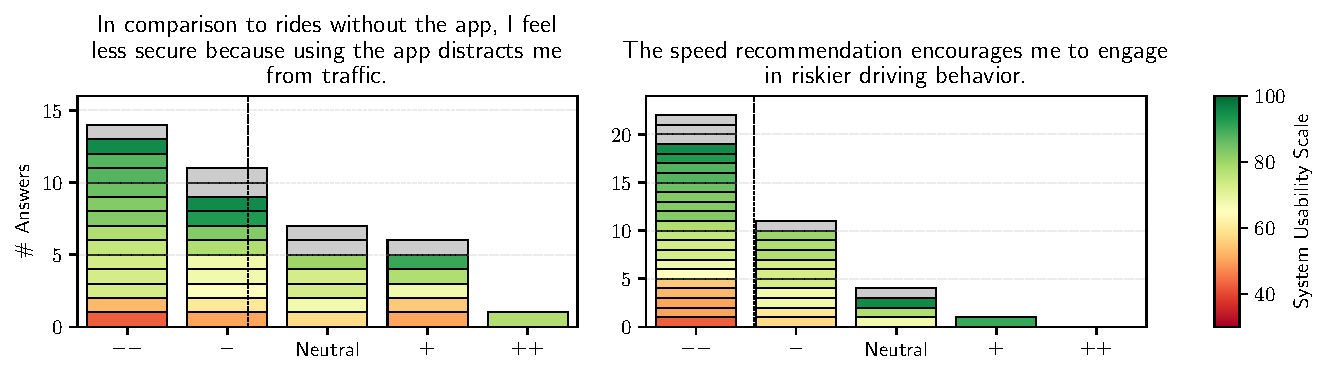
\includegraphics[width=\linewidth]{images/app-usability-questions-app-impact-on-safety.pdf}
\end{figure}
          

\begin{figure}[t]
\caption{Enhanced orientation, comfort, and informedness with the app.}\label{fig:app-enhanced-orientation}
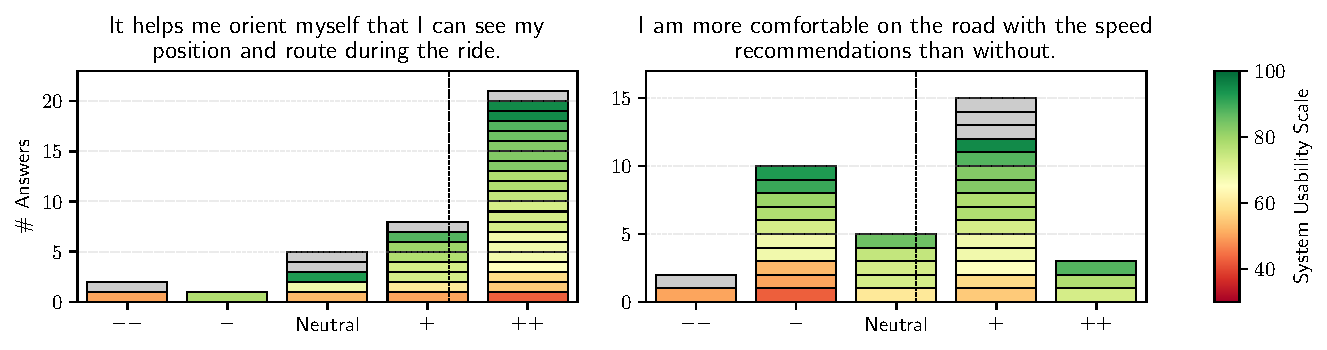
\includegraphics[width=\linewidth]{images/app-usability-questions-app-enhanced-orientation.pdf}
\\
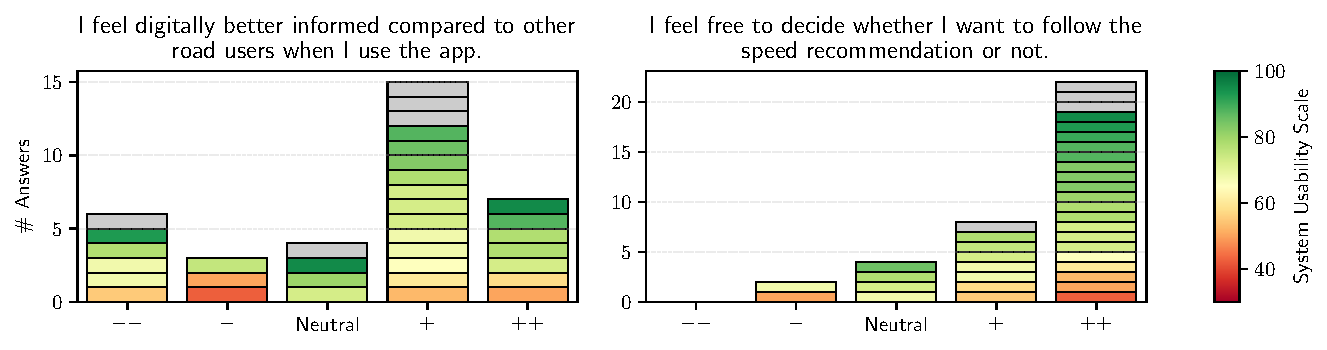
\includegraphics[width=\linewidth]{images/app-usability-questions-app-informedness-freedom.pdf}
\end{figure}

- General user feedback

\begin{figure}[t]
\caption{Negative feedback given in survey.}\label{fig:app-negative-feedback}
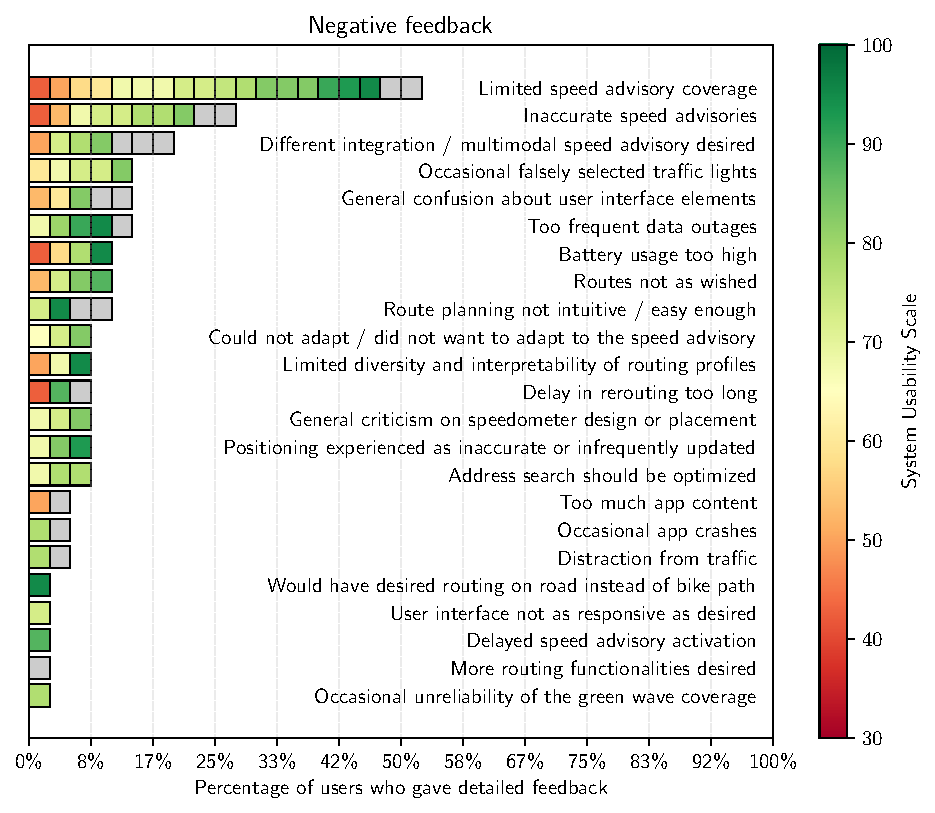
\includegraphics[width=\linewidth]{images/app-feedback-negative.pdf}
\end{figure}

\begin{figure}[t]
\caption{Positive feedback given in survey.}\label{fig:app-positive-feedback}
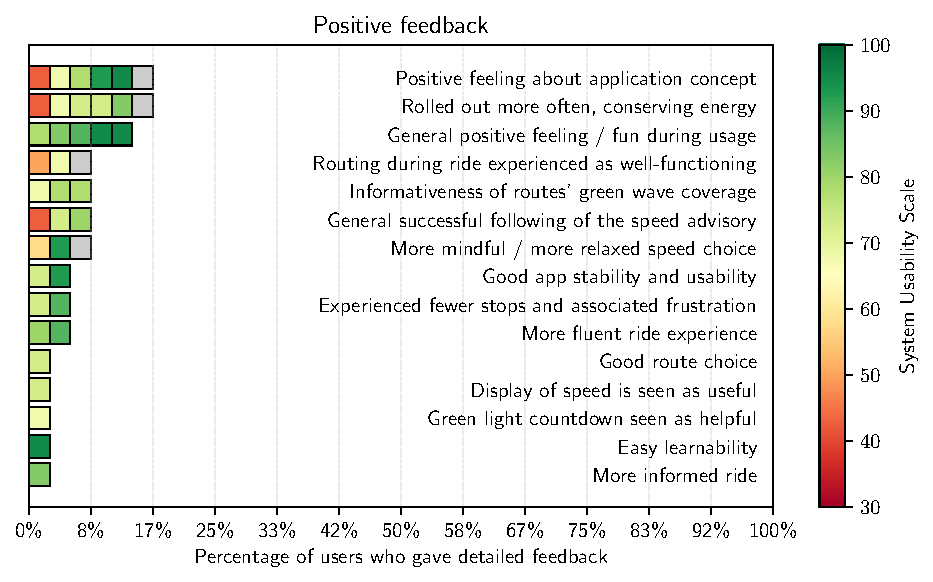
\includegraphics[width=\linewidth]{images/app-feedback-positive.pdf}
\end{figure}


\subsection{Interaction During Ride}

- Interaction during ride

\begin{figure}[t]
\caption{Recorded interaction with the smartphone's screen while in the ride view.}\label{fig:app-user-interaction}
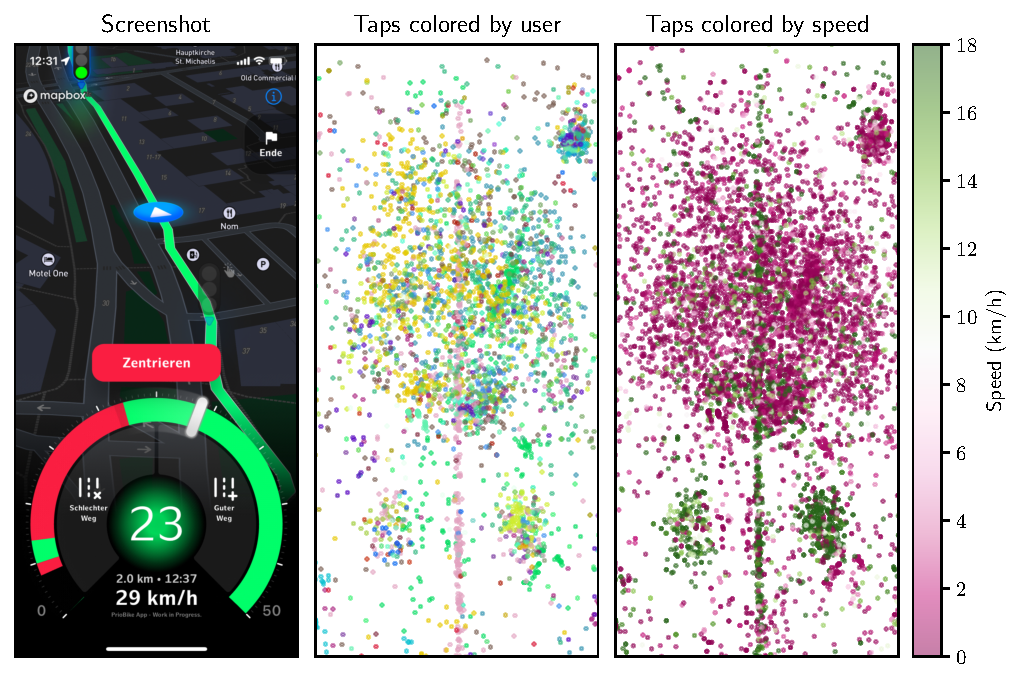
\includegraphics[width=\linewidth]{images/app-user-interaction.pdf}
\end{figure}

- Top 10 tracks by tap rate have > 27 taps/min, but are only approx. one minute long. Maybe they failed to plan a correct route?
- Median is 0.15 taps/minute (IQR: 0.34)
- 765 (57.5\%) of tracks have $\leq$ 2 taps in total (to end ride)

\begin{figure}[t]
\caption{Taps on the screen by currently driven speed and time of entering/leaving the view.}\label{fig:app-user-interaction-speed}
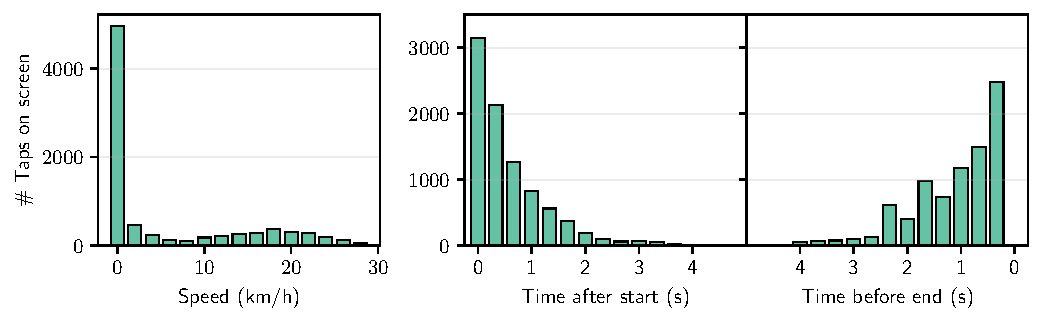
\includegraphics[width=\linewidth]{images/app-user-interaction-speed.pdf}
\end{figure}


\subsection{Measured Impact on Cycling}

- Distinct sgs with GLOSA: 1004
- Distinct sgs in total: 1417
- Distinct sgs without GLOSA: 1060

\begin{figure}[t]
\caption{Measured adherence to the speed advisory and activation distance.}\label{fig:impacts-adherence-activation-distance}
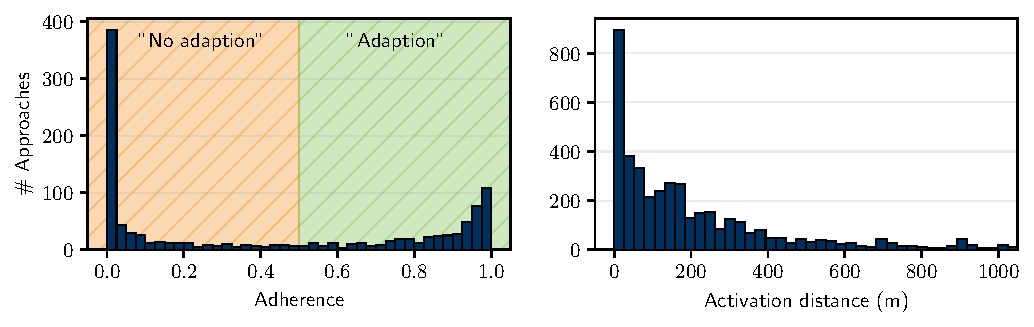
\includegraphics[width=\linewidth]{images/impacts-adherence-activation-distance.pdf}
\end{figure}

- Median activation distance: 133.49766880469255 
- IQR activation distance: 260.667945272357
- Number of trajectories with GLOSA: 1120 
- Number of trajectories without GLOSA: 842
- Median adherence: 0.0 IQR 0.4660847535192057
- No adherence: 283 
- Adherence < 0.5: 638 
- Adherence > 0.5: 482 
- Adherence == 1: 8

\begin{figure}[t]
\caption{Measured speed advisory impact on traffic light approach speed.}\label{fig:impacts-approach-speed}
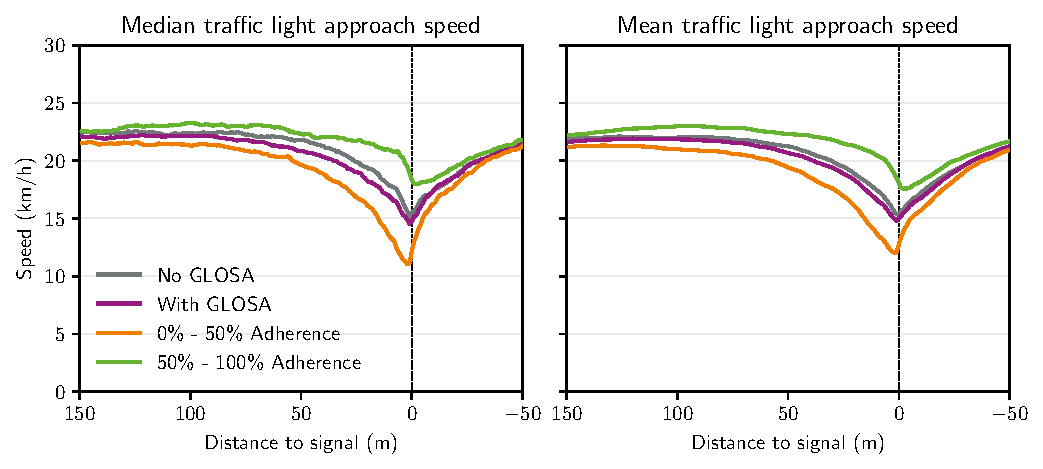
\includegraphics[width=\linewidth]{images/impacts-approach-speed.pdf}
\end{figure}

- Impact on approach speed
- Median speed at 0m with GLOSA: 14.748851498558905 (IQR 12.332427560394335)
- Median speed at 0m no GLOSA: 15.47884898628614 (IQR 12.08553925483405)
- Median speed at 0m no adherence: 12.093527416016059 (IQR 11.731757336342692)
- Median speed at 0m adherence: 18.398685181342955 (IQR 10.33149951069667)

- Resulting energy savings
- Average kJ with GLOSA: 19.24 
- Average kJ with GLOSA and adherence > 50\%: 21.00 
- Average kJ with GLOSA and adherence < 50\%: 17.98 
- Average kJ without GLOSA: 19.79

\begin{figure}[t]
\caption{Distribution of speeds on traffic light approach depending on the adherence level.}\label{fig:impacts-approach-speed-heatmap}
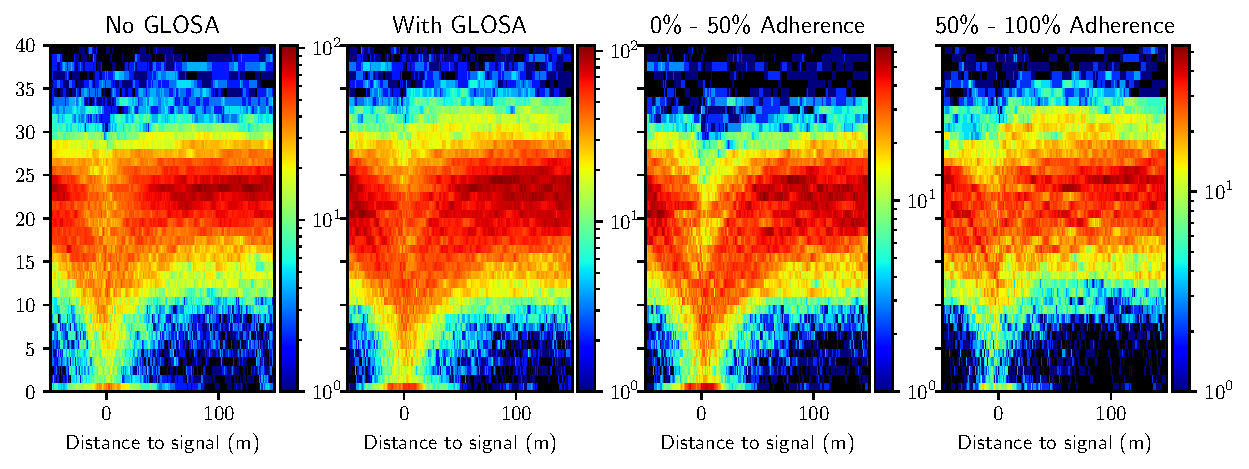
\includegraphics[width=\linewidth]{images/impacts-approach-speed-heatmap.pdf}
\end{figure}

- Stop rate
- No GLOSA: 311 \href{https://file+.vscode-resource.vscode-cdn.net/}{/} 842 (36.94\%) 
- 0\% - 50\% Adherence: 332 \href{https://file+.vscode-resource.vscode-cdn.net/}{/} 638 (52.04\%) 
- 50\% - 100\% Adherence: 102 \href{https://file+.vscode-resource.vscode-cdn.net/}{/} 482 (21.16\%)

- Stop time
- Stopped so many times with GLOSA: 0.26\% 
- Stopped so many times with GLOSA and adherence > 50\%: 0.15\% 
- Stopped so many times with GLOSA and adherence < 50\%: 0.32\% 
- Stopped so many times without GLOSA: 0.25\% 

- If stopped, stopped so long with GLOSA: 23.48s 
- If stopped, stopped so long with GLOSA and adherence > 50\%: 24.90s 
- If stopped, stopped so long with GLOSA and adherence < 50\%: 23.00s 
- If stopped, stopped so long without GLOSA: 23.96s

\begin{figure}[t]
\caption{Example intersection approach utilized for human labeling for cross-validation.}\label{fig:example-trajectory-3.pdf}
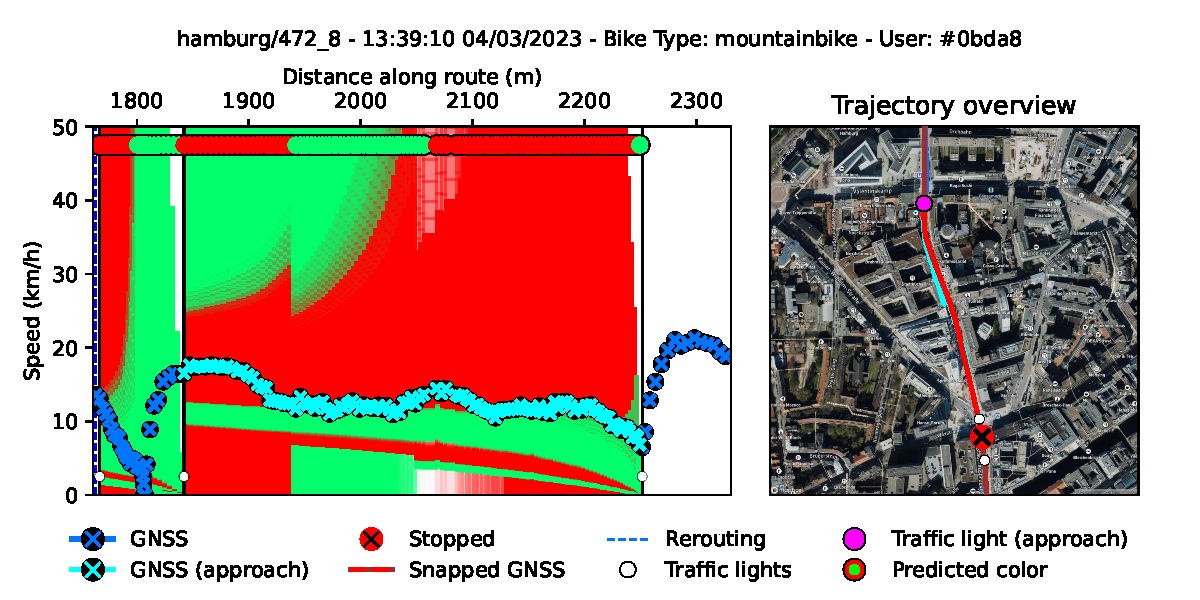
\includegraphics[width=\linewidth]{images/example-trajectory-3.pdf}
\end{figure}

- Total labels: 1,165, persons involved in the process: 5 (equally split)
- Equal decisions: 915
- Unequal decisions: 200
- Decisions where only one person labeled: 50

- Adapted to speed advisory but stopped: 72
- Adapted to speed advisory but did not stop: 447
- Not adapted to speed advisory although possible and stopped: 149
- Not adapted to speed advisory although possible and not stopped: 67
- No adaption possible and stopped: 106
- No adaption possible and not stopped: 74

\section{Conclusions}
